\documentclass{report}


% Language and localization setup
\usepackage[english]{babel}
\usepackage[utf8]{inputenc}
\input{ix-utf8enc.dfu}

% Add graphics support
\usepackage{graphicx}
\usepackage{fixltx2e}


% Add table support
\usepackage{float}
\usepackage{multirow}
\usepackage[table,xcdraw]{xcolor}

% Add caption support
\usepackage{caption}  % Use for \captionof(*) command
\usepackage{subcaption}

% Insertion of whole PDF pages into document
\usepackage{pdfpages}
\usepackage{pdflscape}
\usepackage{afterpage}

% Add robust list support
\usepackage[ampersand]{easylist}

% Change section titles
\usepackage{titlesec}

% Add ToC entries down to X.X.X.X level
\setcounter{secnumdepth}{4}
\setcounter{tocdepth}{3}

% Adds pretty boxes around chapter headings
\usepackage[Glenn]{fncychap}

% \usepackage[sorting=none]{biblatex}

% Adds in support for multiple page styles
\usepackage{fancyhdr}
\usepackage{lastpage}

% Adds header, footer, and footnote support
\usepackage{extramarks}

% Extra math capabilities and symbols
\usepackage{amsmath}
\usepackage{amsthm}
\usepackage{amsfonts}
\usepackage{textcomp}
\usepackage{xfrac}
\usepackage{cool}
\usepackage{cancel}
\usepackage{gensymb}

% Control line and paragraph spacing
\usepackage{parskip}

% Chemical and isotope notation
\usepackage[version=3]{mhchem} 

% Adds cross-references and labeling
\usepackage{refcount}
\usepackage[hidelinks]{hyperref}

% Define units
\usepackage{siunitx}

% Font control
\usepackage{lmodern}
\usepackage{microtype}



% \usepackage{natbib}
\usepackage{etoolbox}
\patchcmd{\chapter}{\thispagestyle{plain}}{\thispagestyle{fancy}}{}{}


\usepackage [autostyle, english = american]{csquotes}
% \MakeOuterQuote{''}


\pdfoptionpdfminorversion=6



% \usepackage{notoccite}


%
% Basic Document Settings
%

\topmargin=-0.45in
\evensidemargin=0in
\oddsidemargin=0in
\textwidth=6.5in
\textheight=9.0in
\headsep=0.25in

\linespread{1.1}

\clubpenalty = 10000
\widowpenalty = 10000

\fancypagestyle{fancyTOC}{
    \lhead{\MakeUppercase{\rightmark}}
  \chead{}
  \rhead{}
  \lfoot{\MakeUppercase{\leftmark} }
  \cfoot{}
  \rfoot{\thepage}
  \renewcommand{\headrulewidth}{0.4pt}
  \renewcommand{\footrulewidth}{0.4pt}
}

\fancypagestyle{fancyacronym}{
    \lhead{LIST OF ACRONYMS}
  \chead{}
  \rhead{}
  \lfoot{LIST OF ACRONYMS }
  \cfoot{}
  \rfoot{\thepage}
  \renewcommand{\headrulewidth}{0.4pt}
  \renewcommand{\footrulewidth}{0.4pt}
}

\fancypagestyle{fancy2}{
% \lhead{\nouppercase{\rightmark}}
 \lhead{\rightmark}
 \chead{}
  \rhead{}
%   \lfoot{\thechapter\ \ \ \nouppercase{\leftmark} }
  \lfoot{\thechapter\ \ \ \MakeUppercase{\leftmark} }
  \cfoot{}
  \rfoot{\thepage}
  \renewcommand{\headrulewidth}{0.4pt}
  \renewcommand{\footrulewidth}{0.4pt}
}


\pagestyle{fancy}
% \lhead{\nouppercase{\rightmark}}
 \lhead{\rightmark}
 \chead{}
  \rhead{}
%   \lfoot{\thechapter\ \ \ \nouppercase{\leftmark} }
  \lfoot{\thechapter\ \ \ \MakeUppercase{\leftmark} }
  \cfoot{}
  \rfoot{\thepage}
  \renewcommand{\headrulewidth}{0.4pt}
  \renewcommand{\footrulewidth}{0.4pt}

  \renewcommand{\chaptermark}[1]{%
  \markboth{#1}{}}



\setlength\parindent{0pt}
\setlength\parskip{1.5ex}





%
% Define Title Page content
%

\title{Preventing a Nuclear ISIL: \\Recommendations for United States Policy}

\date{11 May 2015}

\author{\textbf{Contributing Authors:}\\ \\
James	Bevins\\
% Christopher	Brand - Naughty...\\
Christopher	Brand \\
Grant	Buster\\
Denia	Djoki\'{c}\\
Andrew	Greenop\\
Eric	Harvey\\
Tom	Hickey\\
% \'{A}nth\'{o}n\'{y}	J\'{u}\'{a}r\'{e}z\\
Anthony	Juarez\\
% Azimbek	Jumakulov - Naughty...\\
Azimbek	Jumakulov \\
James	Kendrick\\
% Nicolas	Mertz - Naughty...\\
% Diana	Othman - Naughty...\\
% Scott	Parker - Naughty...\\
% Bushra	Samimi - Naughty...\\
Nicolas	Mertz \\
Diana	Othman \\
Scott	Parker \\
Bushra	Samimi \\
Julie	Stabile\\
Andrew	Voyles\\
Xin	Wang
}



\renewcommand{\part}[1]{\textbf{\large Part 
\Alph{partCounter}}\stepcounter{partCounter}\\}

%
% Various Helper Commands
%

% Useful for algorithms
\newcommand{\alg}[1]{\textsc{\bfseries \footnotesize #1}}

% For derivatives
\newcommand{\deriv}[1]{\frac{\mathrm{d}}{\mathrm{d}x} (#1)}

% For partial derivatives
\newcommand{\simplepderiv}[2]{\frac{\partial}{\partial #1} (#2)}

% Integral dx
\newcommand{\dx}{\mathrm{d}x}

% Alias for the Solution section header
\newcommand{\solution}{\textbf{\large Solution}}

% One sentence of lorem ipsum text
\newcommand{\shortlipsum}{Lorem ipsum dolor sit amet, consectetuer adipiscing 
elit.}

% Pad zeroes for footer numbering
\newcommand\twodigits[1]{%
  \ifnum#1<10 0#1\else #1\fi
}

% Consistant figure references
\newcommand{\figref}[1]{Figure~\ref{#1}}

% Define partial derivative alias
\newcommand{\partialder}[1][2]{frac{\partial u}{\partial t} #1}

% Volume symbol
\newcommand{\volume}{\mathop{\ooalign{\hfil$V$\hfil\cr\kern0.08em--\hfil\cr}}\nolimits}

% Area symbol
\newcommand{\area}{\mathop{\ooalign{\hfil$A$\hfil\cr\kern0.08em--\hfil\cr}}\nolimits}

% Sin and Cos with auto-parentheses 
\newcommand{\sinp}[1]{\sin{\left( #1\right)}}
\newcommand{\cosp}[1]{\cos{\left( #1\right)}}
\newcommand{\expp}[1]{\exp{\left( #1\right)}}




% Make vectors use boldface
\renewcommand{\vec}[1]{\mathbf{#1}}


% Consistant matrix notation
\newcommand{\matr}[1]{\mathbf{#1}} % undergraduate algebra version
% \newcommand{\matr}[1]{#1}          % pure math version
% \newcommand{\matr}[1]{\boldsymbol{#1}}     % ISO complying version


% \newcommand{\myparagraph}[1]{\paragraph*{#1}\mbox{} \\}
\newcommand{\myparagraph}[1]{\paragraph*{#1\\}}



\makeatletter
% Make common definition of mean
\newcommand*\mean[1]{\overline{#1\raisebox{3mm}{}}}

% \def\toclevel@subsubsection{2}


\makeatother









\begin{document}

% \pagenumbering{arabic}
% 
% 
% \maketitle
% 
% 
% \tableofcontents
% 
% \thispagestyle{fancyTOC}


\pagenumbering{alph}
\begin{titlepage}
\maketitle
\thispagestyle{empty}
\end{titlepage}
\pagenumbering{arabic}

\pagestyle{fancyTOC}


\tableofcontents
% \thispagestyle{fancyTOC}
\pagestyle{fancyTOC}




\listoffigures
\thispagestyle{fancyTOC}


\listoftables
\thispagestyle{fancyTOC}

\newpage


\pagestyle{fancyacronym}

\chapter*{List of Acronyms}
\pagestyle{fancyacronym}


{\parskip=0.5ex AAPA - American Association of Port Authorities

ALARA - As Low As Reasonably Achievable

AP - Additional Protocol

AQI -  al-Qaeda in Iraq

ASP - Advanced Spectroscopic Portal Monitor

CBP - U.S. Customs and Border Protection

DDA - Department of Disarmament Affairs

DHS - Department of Homeland Security

DIA - Defense Intelligence Agency

DNDO - Domestic Nuclear Detection Office

DoD - Department of Defense

DoE - Department of Energy

DoJ - Department of Justice

DoS - Department of State

DoT - Department of Treasury

DTRA - Defense Threat Reduction Agency

ETRI - Expanded Threat Reduction Initiative

FATF - Financial Action Task Force

FBI - Federal Bureau of Investigation

FBIS - Foreign Broadcast Information Service

FPCON - Force Protection Condition

GA - General Assembly

GEOINT - Geospatial Intelligence

GTRI - Global Threat Reduction Initiative

HEU - Highly Enriched Uranium

HUMINT - Human-Source Intelligence

IC- Intelligence Community

ICE - Immigration and Customs Enforcement

IMINT - Imagery Intelligence 

IAEA - International Atomic Energy Agency 

IS - Islamic State

ISI - Islamic State of Iraq

ISIL - Islamic State of Iraq and the Levant

ISIS - Islamic State of Iraq and Syria

ISN - Bureau of International Security and Nonproliferation

ISOO - Information Security Oversight Office

ISTC - International Science and Technology Center

ITDB - Incident and Trafficking Database


JTWJ - Jama'at al-Tawhid wal-Jihad 

LEU - Low Enriched Uranium


LLNL - Lawrence Livermore National Laboratory

MASINT - Measurement and Signature Intelligence 

NASIC - National Air and Space Intelligence Center 

NFAA - Nuclear Forensics and Attribution Act

NGA - National Geospatial-Intelligence Agency 

NNSA - National Nuclear Security Administration 

NPR - Nuclear Posture Review

NPT - Non-Proliferation Treaty

NRO - National Reconnaissance Office

NSA -National Security Agency

NSC - National Security Council  

NTNFC - National Technical Nuclear Forensics Center

ODNI - Office of the Director of National Intelligence

OIR - Operation Inherent Resolve

OMB - Office of Management and Budget

OSINT - Open-Source Intelligence

PNNL - Pacific Northwest National Lab

RDD - Radiological Dispersal Device

RPM - Radiation Portal Monitor

SC- Security Council

SIGINT - Signals Intelligence 

SLD - Second Line of Defense

SNM - Special Nuclear Material

SOCOM - U.S. Special Operations Command

UN - United Nations

WMD - Weapons of Mass Destruction}

\newpage


\thispagestyle{empty}

\topskip0pt
\vspace*{\fill}



\begin{center}
 \enquote{\emph{One of the most important lessons of the Cold War was that incessantly worrying about the low-probability/high-impact cases was a mistake.}}  
 
 
 
 - Kenneth Pollack 

\end{center}

\vspace*{\fill}



\newpage

\pagestyle{fancy2}


\chapter{Executive Summary}






This report addresses the possibility of the Islamic State of Iraq and the Levant (ISIL) becoming a nuclear threat to the United States and its allies by the acquisition of nuclear weapons, special nuclear material, or radiological dispersal devices. In accordance with President Obama's National Security Strategy, which states that \enquote{there is no greater threat to the American people than \ldots the pursuit of nuclear weapons by violent extremists \ldots}, this report informs a policy targeted at the prevention of such a calamity \cite{Obama2010}.


The unique history, ideology, and current geographic influence of ISIL are illustrated. ISIL is unlike any adversary the United States has had in the past, and therefore the need to understand and prevent any pathways to acquisition of nuclear material that could lead to wielding a nuclear weapon is imperative.

Policy recommendations for preventing a nuclear capable ISIL were developed by modeling the steps ISIL would have to take to procure a nuclear device, from the inception of the idea, to staging and detonation. Each recommendation is meant to target a specific chain of a  logic model developed in this report, with the ultimate goal of destroying all paths ISIL may have to a nuclear device. 



This report has illustrated the details of policy recommendations focused on preventing the low-probability / high-consequence event of ISIL becoming a nuclear threat. To target all possible pathways, this report has made policy recommendations - new ones, as well as additions to existing policy - in an effort to prevent weapons theft or purchase, the strengthening of ISIL foundational capabilities for indigenous development, or the acquisition of radiological material for use in a radiological dispersal device. These policies are  summarized here:

\begin{easylist}[enumerate]
& Policies specifically targeting \textbf{indigenous development:}
&& Targeting of foundational capabilities	
% &&& Income 
% &&& People and expertise 
% &&& Infrastructure
&& IAEA monitoring 
% &&& Additional Protocol – push for more signatures 
% &&& International and Trafficking Database – push for increased cooperation
& Policies specifically targeting \textbf{proliferation through theft/purchase:}
&& IAEA monitoring 
% &&& International and Trafficking Database – push for increased cooperation
% &&& Additional Protocol – push for more signatures 
&& Global Threat Reduction Initiative (GTRI) 
% &&& Push for the cooperation of more nations
&& Strengthening of multilateral security agreements
&& Nuclear Forensics Attribution Act (NFAA)
% &&& Explicit declaratory policies, explicit deterrence 
&& United Nations Security Council Resolution (UNSCR) 1540 
% &&& Additional provisions and security expert group
&& Second Line of Defense (SLD)
% &&& Additional foreign ports
& Policies specifically targeting \textbf{delivery/staging:}
&& Military Force Protection Condition (FPCON)
% &&& Increased military base safety
&& Advanced Radiation Portal Monitor (RPM) Plan
% &&& Increased domestic port monitoring and advanced monitor development
&& Second Line of Defense (SLD)
% &&& Monitor additional foreign ports
\end{easylist}



% The risk of ISIL becoming a nuclear threat is a low-probability/high-impact case. Thus, the policy recommendations made in this report are targeted to reducing the already-low probability of nuclear acquisition as close to zero as possible. This report therefore also illustrates a dissenting opinion, offering a viewpoint that the resources allocated to the recommended policies could be disproportionate to the reality of the risk, and that current policies addressing the risk are adequate.


The recommendations that have been illustrated in this report rest on the assumption that a nuclear ISIL needs to be prevented at any cost. A dissenting viewpoint has been offered and explored, and recommends focusing efforts on dismantling ISIL as a movement instead of dedicating disproportionate resources to an unknown probability of nuclear acquisition. Regardless of the philosophy on how to allocate funding to implement policy options, it is at the very least prudent to spend efforts on reducing knowledge uncertainty of possible ISIL-related nuclear event. Part of the low-hanging fruit of increasing preparedness and U.S. response capability (especially keeping in mind the cost, feasibility, and tradeoffs of policy implementation) is the assessment of possible nuclear outcomes, such as this report has done. However large or small the perceived risk, the work contained in this report contributes to the knowledge of prevention and response to the possibility of a nuclear ISIL.


Therefore, the dissenting opinion recognizes that the marginal cost to implement the proposed policies outweigh the marginal benefit and recommends to not repeat the mistakes of history by implementing the proposed policies of this report. As Ken Pollack once said, \enquote{One of the most important lessons of the Cold War was that incessantly worrying about the low-probability / high-impact cases was a mistake.}  
Instead, it is proposed that the U.S. implements no changes to U.S. policy specifically to prevent the low probability event that is ISIL obtaining nuclear weapons. This would entail \enquote{staying the course} with President Obama's current policy of disrupting, degrading, and ultimately destroying ISIL as a necessary and sufficient condition to prevent nuclear weapon acquisition, while not losing focus on the real ISIL national security challenges \cite{WhiteHouse2014}.





% The ISIL nuclear threat is, by definition, a low-probability / high-impact case as this report has shown.  Developing nuclear weapons amidst crippling sanctions, airstrikes, and a dedicated opposition has never been done, despite several nation states attempting to do so.  Therefore, we choose to not repeat the mistakes of history and propose that no changes to U.S. policy be implemented to prevent ISIL from obtaining nuclear weapons.






\chapter{Introduction to ISIL}





   
   

    
    
    
    \section{Background}
    
    \subsection{History}
    
    The Islamic State of Iraq and the Levant (ISIL)\footnote{ISIL is also known as Daesh, the Islamic State of Iraq and Syria (ISIS),  the Islamic State of Iraq and al-Sham, or simply the Islamic State (IS).} can be traced back to the founding of the militant Jihadist group Jama'at al-Tawhid wal-Jihad (JTWJ) by the Jordanian terrorist Abu Musab al-Zarqawi in 1999. al-Zarqawi's JTWJ gained both fame and notoriety throughout Iraq in the early 2000s for  a campaign of brutal beheadings and suicide bombings against both Sunni and Shia targets \cite{Zelin2014}. Despite initial conflicts with al-Qaeda in ideology and methodology, al-Zarqawi pledged allegiance to Osama bin Laden and al-Qaeda in 2004 to coordinate  their efforts to overthrow apostate Arab regimes, as well as the Western powers. To mark this pledge, al-Zarqawi renamed his group al-Qaeda in Iraq  (AQI) \cite{Gambill2004}. Despite this commitment, tensions and occasional armed conflicts between the two groups remained.
    
    Throughout the many conflicts in Iraq in the remainder of the 2000s, AQI underwent many changes in leadership, ideology, and name. These changes, primarily the deaths of much of its upper leadership (including al-Zarqawi), were caused by a combination of military pressure from U.S. troops, multiple disagreements  with bin Laden's al-Qaeda, and backlash from other Sunnis in Iraq \cite{Zelin2014,Kahl2008}. As a result of this, AQI was reorganized as the Islamic State of Iraq (ISI) in 2007, with Abu Bakr al-Baghdadi as it newly appointed leader \cite{Zelin2014,Shadid2010}. Under the new leadership of al-Baghdadi, ISI broke a period of regional détente with al-Qaeda (following the death of Osama bin Laden in August 2011), driving a further wedge between the two groups by al-Baghdadi's refusal to pledge allegiance to the new leader of al-Qaeda, Ayman al-Zawahiri \cite{Al-Jawlani}. In April 2013, this division resulted in  al-Baghdadi announcing that ISI would be extending its reach into Syria, and changing its name to the Islamic State of Iraq and al-Sham, or the Islamic State of Iraq and the Levant \cite{Zelin2014,Al-Hussaini2013}. In June 2014, al-Baghdadi declared ISIL a global Caliphate, with himself as its Caliph \cite{Mortada2014,TheWeek2014}. To understand the significance of this declaration, let us consider the history and role of Caliphs and Caliphates in Islam.
    
    


\subsection{Legitimacy of the Caliphate}

The origin of the Islamic concept of a Caliphate can be traced back to the foundations of Islam by Muhammad, and his organization of the Arabian peoples (who became the first Muslims) into a single theocratic society  \cite{schmidt2004great,holt1977cambridge}. This society was called a Caliphate, and was envisioned as a single state, led by a divinely-appointed leader called a Caliph, with full authority over government, religion, and military strength for all Muslims worldwide \cite{lapidus2002history}. Furthermore, as based upon the teachings of the Quran and Hadith, the Caliphate is obligated to conquer the world through Jihad, but the West in particular, creating a global Caliphate with all peoples either converted into Islam, or unbelieving subjects of the Caliphate \cite{dawood2003koran,arabi2008divine,karsh2007islamic}. Following the death of Muhammad in 632, there was a brief period of consensus over leadership, but a dispute quickly arose over who would lead the Muslims as Caliph, a schism that exists still today. Sunni Muslims believe  Abu Bakr, the father-in-law of Muhammad, was the rightful successor and Caliph, and that future Caliphs should be elected by the Muslim community. In contrast, Shia Muslims believe  Ali, the son-in-law of Muhammad, was the rightful successor and Caliph, and that future Caliphs should be direct descendants of Ali \cite{karsh2007islamic,schmidt2004great}. 

Initially, the Sunnis had a majority, with Abu Bakr assuming power as the first Caliph. Following the death of Abu Bakr in 634, two other Sunni Muslims were selected as the next two Caliphs \cite{schmidt2004great}. After decades of fighting and assassinations between these two early sects, Ali became Caliph in 656, but his reign was filled with great internal chaos. Following his death in 661, the reign passed on to his son, Hasan, ushering in centuries of expansion under the dynastic Caliphates, the Umayyad Caliphate (661-750), and Abbasid Caliphate (750-1517) \cite{schmidt2004great,oliver2009caliphate}. By 1517, the Abbasid Caliphate had its seat of power located in Cairo; when the Ottoman Empire annexed Cairo, the Ottomans usurped the office of the Caliph from that last Abbasid Caliph. This ushered in a period of even more rapid expansion under  the Ottoman Caliphate, which lasted until 1924, when Turkey abolished the Caliphate as part of secular and constitutional reform following the Treaty of Versailles of 1919 \cite{schmidt2004great,ozoglu2011caliphate}. The remainder of the Middle East was divided up into largely British and French protectorates, which remains as a point of grievance for many Muslims.

Since the abolition of the Caliphate, there have been several attempts to bring about a new Caliphate, notably the  1928 efforts of the nascent Muslim Brotherhood in Egypt \cite{Tolson2008,gabriel2008they}. However, there have been no successful attempts in the modern era, until  June 2014, when al-Baghdadi declared ISIL a global Caliphate, with himself as its Caliph and the rightful successor of the Ottoman Caliphate, citing the campaigns and expansion of ISIL as signs that ISIL is a spiritual successor of the Ottoman Caliphate \cite{Mortada2014,TheWeek2014}.  This declaration has received great criticism from not only the international community \cite{Gomes2007}, but from Muslims and other Jihadist groups as well \cite{Mandhai2014,Moore2014}. ISIL's many acts of terrorism, war crimes, and human rights violations have drawn strong criticism from the international community. From within the Muslim community, the criticism stems from the ISIL Caliphate being invalid under Islamic law, as they do not have a direct line of succession from the previous Ottoman Caliphate. In addition, many Muslims and Muslim clerics fear that the brutal and violent operations of ISIL, as well as its extremely literal and orthodox interpretation of the teachings of  the Quran and Hadith, are \enquote{rejected by most mainstream Islamists because they feel it damages their cause to establish an Islamic system through peaceful means} \cite{Mandhai2014}. Some Muslims feel that ISIL's brutal slaughter of Muslims and non-Muslims alike distorts the teachings of the Quran and Hadith and the present is not the correct time for a Muslim global Caliphate. Some believe Muslims  should currently seek a time of peace, strengthening themselves for a time of war against the West in the future \cite{schmidt2004great,Moore2014,Wood2015}.

    


    \subsection{Ideology}
    
    ISIL is an adherent to the Salafi movement of Sunni Islam \cite{Bradley2015}, itself a very orthodox school of thought among Muslim theology.  As such, it promotes a reform of Islam back to its roots with Muhammad, and an extremely literal interpretation of the Quran and Hadith \cite{Hassan2015}. Many modern Jihadist groups are devout adherents to Salafi Islam, which requires that all true believers live the tenets of the Quran to the letter. Salafists  advocate Jihad and the conquest of all peoples (specifically the West) by forcible conversion, execution, or subjugation through conquest, driving towards a global Caliphate. ISIL shares these beliefs with other modern Islamic Jihadist groups, including the Muslim Brotherhood and al-Qaeda, due to its support of religious violence and terrorism \cite{schmidt2004great,gabriel2008they,Hassan2015,Moussalli2009}.
    
    One significant difference between ISIL and other mainstream Sunni Muslims is that ISIL violently condemns all Muslims who disagree with its interpretations as infidels and apostates, promoting  sectarian violence for deviating from the \enquote{pure Islam} that ISIL follows. They also advocate this same violence against journalists, civilians, relief workers, and any other individuals or groups whom ISIL believes are supporting any infidel \cite{Wood2015,Hassan2015,AustralianNationalSecurityAttorney-GeneralsDepartment2014}. Many of the atrocities that have so shocked the world - beheadings, burnings, forced marriages - result from this commitment of ISIL to live the tenets of the Quran to the letter. It is these extreme levels of  violence (sectarian and otherwise) that has earned ISIL condemnation from mainstream Sunni and Shia clerics, as ISIL's public show of fundamentalist Islam gives Islam a violent appearance in the eyes of the global community \cite{Mandhai2014}.
    
    In line with their  orthodox and literal interpretation of Islamic teachings, ISIL  has a strict literal interpretation of Islamic  end-times theology. ISIL teaches that the world is currently in the beginning of the end times, and that their actions are intended to hasten the arrival of Imam Mahdi, a Muslim messianic figure prophesied by Muhammad in the Hadith, whose rule will precede the end of all times \cite{arabi2008divine,Wood2015}. ISIL believes that when the Mahdi arrives, the global Caliphate (with ISIL at its head)  will \enquote{await the army of \enquote{Rome,} whose defeat at Dabiq, Syria, will initiate the countdown to the apocalypse} \cite{Wood2015}. However, from the declarations of ISIL, it is unclear what \enquote{Rome} actually represents - America, the West, Turkey (whose abolishment of the Ottoman Caliphate is seen as an act of supreme treachery against all Muslims, and earns them a particular vehemence from ISIL), any \enquote{apostate} group from ISIL's standpoint, or some other institution which represents an archetype of anti-Caliphate authority to ISIL \cite{Mortada2014,Wood2015}. 
    
    
    


\subsection{Land}

ISIL controls land in Iraq and Syria, including several cities that include Arbil and Mosul in Iraq and Aleppo and Raqqa in Syria \cite{McFate2015}.  Iraqi military forces, supported by U.S. airstrikes, have recently pushed ISIL out of Tikrit in Northern Iraq, and are now gearing up to push ISIL out of various location in Anbar province, including Falluja and Ramadi \cite{Nordland2015}.  In April 2015, the Pentagon released an assessment that Iraqi forces had pushed ISIL out of roughly 25\% of the territory it had seized in advances during 2014 - an area that represents between 5,000 and 6,500 square miles \cite{Michaels2015}.  ISIL's territory is pictured in \autoref{fig:current_territory2}, with indications of the areas in which ISIL territory has been rolled back in the first several months of 2015. 


\begin{figure}
 \centering
 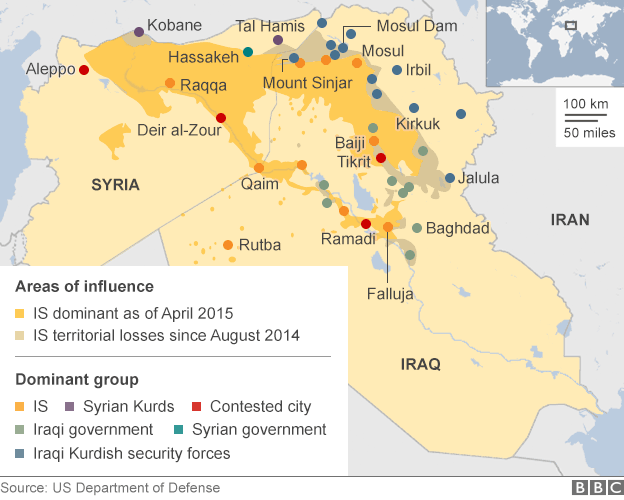
\includegraphics[trim = 0cm 0cm 0cm 0cm, clip,scale=0.6]{./figures/current_territory.png}
   \caption{Current ISIL Territory \cite{BBC2015a}}
     \label{fig:current_territory2}
\end{figure}


\subsection{People}

ISIL has as many as 31,500 fighters in Iraq and Syria, and roughly 19,000 of these are foreign recruits from 90 countries \cite{Sengupta2014,TheEditorialBoard2015}. ISIL has called publicly on Muslims from the world over to join the Caliphate as part of their religious duty as true believers \cite{Stern2015}. In order to recruit foreign fighters - who are often more ideological than the average Syrian rebel - ISIL propaganda is frequently translated into English, French, German, Russian, Indonesian, Urdu, and other languages \cite{Stern2015}. ISIL also recruits through sophisticated modern communication techniques and through representatives in countries around the world in Muslim diaspora populations \cite{Masi2014}.  The majority of foreign fighters originate in Muslim countries in the Middle East and North Africa, with especially high representation from Tunisia and Saudi Arabia. A typical foreign ISIL fighter is a male between the ages of 18 and 29, but may be as young as 15 \cite{Stern2015}.

ISIL also recruits heavily from the West. The U.S. State Department knows of dozens of U.S. citizens fighting for ISIL, and the British government estimates that roughly 500 British citizens have become foreign fighters in ISIL's ranks \cite{Masi2014a}.  In order to join ISIL, recruits from the west must have a jihadi mentor, which can be found online through ISIL's media center or through ISIL supporters in their communities \cite{Masi2014a}.  Many of these western recruits have entered ISIL territory through Turkey \cite{Masi2014a}.  These western terrorist fighters raise concerns that they will return home radicalized and attempt to attack the U.S. homeland \cite{Patrick2014}. 

Decades of psychological research have failed to produce a profile of who becomes a terrorist \cite{Stern2015}. Despite this, there are several pathways to becoming a foreign jihadist, with both internal and external motivations. Foreign terrorist fighters often mention as external motivations specific military conflicts that inspired them to join terrorist groups. Internal motivations include a sense of belonging, the opportunity to take on a new identity, adventure, or money \cite{Stern2015} Recent ISIL video propaganda films demonstrate a startling level of production value that may indicate that the group is recruiting and possibly paying individuals with specialized skills. Taken together, these findings demonstrate that ISIL attracts not only fighters, but also individuals with specialized skills sets, and it does so through both payment and through cultivating a sense of belonging for Muslim immigrants in Western countries and throughout the world \cite{Patrick2014}. 



\subsection{Income}

ISIL has a number of key sources of income, which may be categorized into five key groups, listed in order of magnitude \cite{Report2015}:


\begin{itemize}
\item \textbf{Illicit proceeds from occupation of territory, including oil, extortion, and bank looting:} ISIL's sophisticated extortion racket is similar to that of organized crime rings. ISIL uses force to gain and control resources, including banks, oil and phosphates, agriculture, and archeological sites \cite{Report2015}.
\item \textbf{Kidnapping for ransom:} Reports indicate that ISIL has kidnapping hundreds of people, including Iraqis, Syrians, local ethnic minorities, Westerners, and East Asians. While ISILs murdering of hostages was garnered widespread attention, they have also been effective in extracting ransom payments, with revenue estimated between U.S. \$20 million and \$45 million \cite{Report2015}.
\item \textbf{Donations:} While revenue from external donations has been a relatively small portion of ISIL's income, it has recently been growing in importance. In addition to donations from the Gulf, there is also risk that wire transfers to charitable foundations operating in ISIL territory end up in ISIL's hands \cite{Report2015}. 
\item \textbf{Material support from foreign fighters:} In some instances, foreign terrorist fighters collect money in their home countries and uses it to provide monetary support to ISIL \cite{Report2015}.
\item \textbf{Online fundraising:} While fundraising through modern communications networks is a relatively small  piece of ISIL's income, the group has shown a strong ability to use social media sites such as Twitter and online crowd funding to support its operations \cite{Report2015}.
\end{itemize}


ISIL's operations have been largely self-sustaining, relying on oil income and other criminal and terrorist activities that generated millions of dollars per month \cite{TheWallStreetJournal2014}.  However, recent reports indicate that U.S. Operation Inherent Resolve has disrupted ISIL income streams considerably. The Pentagon reported in early February 2015 that ISIL's main source of income is no longer oil \cite{AlArabiyaNews2015}.  Pentagon spokesperson Rear Admiral John Kirby told reporters during press briefing that following months of airstrikes in the territory it controls, ISIL's oil income was being degraded, and that the group's primary source of income had shifted to donations and trade on black markets \cite{AlArabiyaNews2015}.  


 
    


\section{Goals}


Since ISIL began to seize power and land in Iraq and Syria, many of studied what exactly drives the organization. Perhaps the most complete discussion of the group's motivation comes from Graeme Woods' article \enquote{What ISIL Really Wants,} which appeared in the March 2015 issue of The Atlantic \cite{Wood2015}. In assessing ISIL and its goals, it is first necessary to recognize its differences with other militant Islamic terrorist organizations. 



The strict brand of Salafism which ISIL espouses has also led to another important distinction between ISIL and other terrorist organizations: the establishment of a Caliphate, with Abu Bakr al-Baghdadi as Caliph. A Caliphate is a homeland for Muslims, and ISIL believes that its establishment is necessary for it to truly follow the tenets of Islam. While other terrorist organizations were content to live amongst the people in various countries, ISIL has seized territory and established a government. In their orthodox and literal interpretation of Islam, the division of the Middle East into its current countries was driven by Western countries, and is therefore fundamentally illegitimate and cannot be tolerated. 

The taking and protection of territory by ISIL is one of its core goals. Under the tenets of Salafism, a Caliphate cannot exist without land, and so maintaining a geographic foothold is fundamental to the existence of ISIL. Without it, their caliphate will cease to exist. 

Much discussion has surrounded the flow of foreign fighters into ISIL controlled territory. Again, this is rooted in the groups' religious beliefs. According to Salafism, once a caliphate is established, all true believers must move to it, unless completely unable to do so. 

ISIL poses a more direct threat to its neighbors than to the U.S. homeland. While many foreigners with Western passports have pledged allegiance to ISIL, they often do so with no intent to return, as illustrated by the common burning of passports once individuals reach ISIL territory. Additionally, ISIL must continue to expand, taking territory from \enquote{illegitimate} governments, in order to maintain its own legitimacy as a Caliphate. 


\subsection{What Makes this Different than Traditional Non-Proliferation Efforts?}

Unfortunately, the U.S. cannot use the same nuclear strategies it has in the past to deal with a nuclear ISIL.  The main focus of U.S. nuclear policy since the collapse of the Soviet Union has been non-proliferation.  There has not been as strong of a focus on deterring attacks from an adversary that already has nuclear capabilities \cite{Bracken2013}. However, even before the fall of the Soviet Union, deterrent strategies, such as counterforce, counter value, and mutually assured destruction, were tailored to deter an enemy state, not an extremist group.  Deterrence can only happen if the adversarial group/state thinks that the punishment received from the U.S. will outweigh the benefits of detonating a nuclear weapon \cite{kaplan1991wizards}.  It is unlikely that the U.S. will ever be able to make a threat that can deter ISIL.  Unlike the Soviet Union and other nuclear states, ISIL is made up entirely of militants who will die in defense of their religion and their caliph.  Death is not something that members of ISIL, or any other terrorist group, fear; it is something they celebrate.  They believe they will be rewarded in the next life for what actions on earth.  Even the threat of bombing by the U.S. and death will not deter them.  If they have reached the point of weapon acquisition, they have already ignored the United States' threats of massive retaliation and will likely continue to ignore any future threats.  For this reason, deterrence will be ineffective if ISIL acquires a bomb, so the U.S. must focus on other methods of stopping ISIL from detonating the weapon \cite{Sanderson2015}.






\subsection{ISIL's Potential Targets (\enquote{Declaratory Policies})}

Because of ISIL's ideology and need to maintain territory (as outlined above), if ISIL were to obtain a nuclear device, it is more likely that ISIL will select targets in its immediate vicinity rather than attempt an attack on the U.S. homeland. However, with that being said, the U.S. has many allies and interests in the region, and must therefore still work to counter the possibility that ISIL will obtain a nuclear device. Additionally, it is possible that ISIL will obtain a nuclear device solely to use as a threat or deterrent. The panic that would occur if ISIL obtained a nuclear device cannot be overstated, and merely having a device can help further ISIL's objectives.


\section{Global Relationships} \label{sec:global_rels}





In assessing how ISIL may acquire a nuclear weapon, it is necessary to consider potentially helpful alliances and allies, as well as their enemies.  As with most things related to ISIL and the Middle East, this is not necessarily as straightforward as one would assume.  While some relationships are fixed points of reference, most are dynamic and characterized by opportunism, both on the part of ISIL and the organization or state who seeks to gain some benefit from supporting or opposing them.  The following discussion is not intended to be all encompassing but instead will focus on key players and how they may help or hinder ISIL's nuclear ambitions.  

At first glance, the strategic landscape does not look favorable to ISIL as depicted in \autoref{fig:ISILRelationships} below.  While somewhat dated, it serves a decent representation of some of the key groups and states that are in direct conflict and collaboration with ISIL.  ISIL's key relationships can be broadly grouped into three categories:  countries and groups at war with ISIL, former or potential future allies, and groups that support ISIL.  

 \begin{figure}
 \centering
 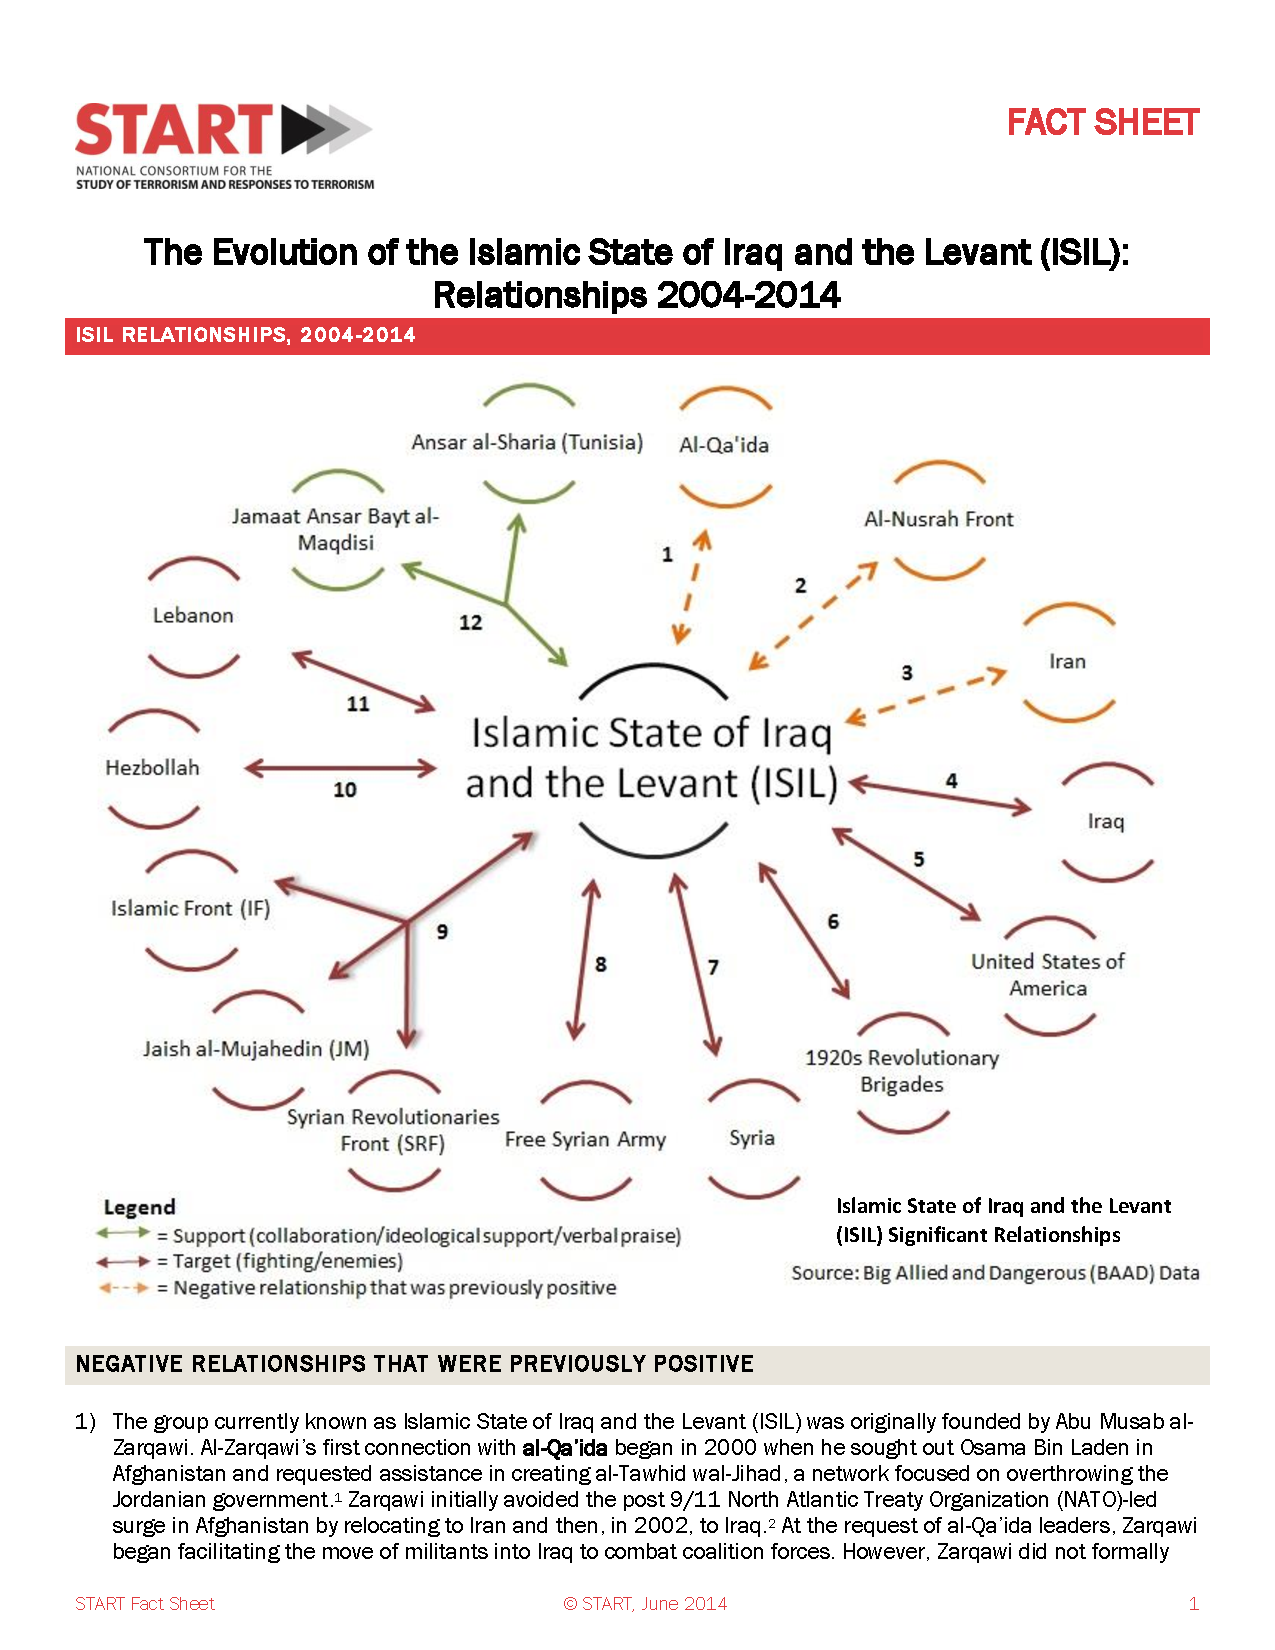
\includegraphics[trim = 0cm 5.9cm 0cm 5.35cm, clip,scale=0.6]{./figures/ISILRelationships.pdf}
   \caption{ISIL relationships as of mid-2014.  Note the figure uses the alternative name of ISIL that was preferred by the Obama administration for ISIL \cite{NationalConsortiumfortheStudyofTerrorismandResponsestoTerrorism2014}}
     \label{fig:ISILRelationships}
\end{figure}



% \subsection{Countries and Groups at War with ISIL}

ISIL has many enemies, indeed many more than are graphically depicted in \autoref{fig:ISILRelationships}.  As of January 2015, the anti-ISIL coalition led by the U.S. included 62 nations and groups including the U.S., Canada, Iraq, Jordan, Bahrain, Saudi Arabia, UAE, France, Germany, United Kingdom, Australia, Belgium, Denmark, Italy, Czech Republic, Albania, Netherlands, Estonia, Hungary, Turkey, and Lebanon, all of whom have carried out or supported military operations against ISIL \cite{Wordsworth2015}.  Additionally, although not allied with the U.S. coalition, Syria, Iran, and various Kurdish, Shia, and Sunni militias in Syria and Iraq have opposed ISIL \cite{Mooney2014}.  Despite this broad coalition, there are many unlikely allies in the list which present potential seams for ISIL exploitation  through propaganda or military action.  For example, strikes against ISIL in Syria benefit the Assad regime while U.S. trained rebels could turn on and attack the Assad regime \cite{Shinkman2015}.  Officially, the U.S. supports the removal of the Assad regime albeit without direct military intervention on part of the U.S. \cite{Shinkman2015}.  Similarly, U.S. air strikes and intelligence have supported Iran and Iraqi Sunni and Shia militias (including several that once fought U.S. forces) in their campaigns against ISIL \cite{Chulov2014}.  While these uneasy alliances have placed pressure on ISIL, it is unclear if they can be sustained over the timeframe that would be necessary to defeat ISIL and prevent their acquisition of a nuclear weapon. Sustaining these alliances would be especially difficult if ISIL were to turn its formidable propaganda machine to breaking some of these fragile links.


Additionally, there are longstanding mistrust, perceptions, and illicit alliances that could cause large fissures  without the help of ISIL.  While the Iraqi government is cooperating with the U.S. in battling ISIL, some clerics and government officials have publicly claimed the CIA was responsible for the rise of ISIL \cite{Kirkpatrick2014}.  Whether this is true is largely irrelevant if the mere perception affects the extent of U.S. - Iraqi cooperation against ISIL, especially if the need would arise to place U.S. troops in combat.  Other reports have the Turkey military providing safe travel and weapons for ISIL fighters attacking Kurdish forces, which have been a thorn in the side of Turkey \cite{Guiton2014}.  Finally, it appears that wealthy Saudis, who have a history of funding terrorist organizations, are continuing to provide ISIL with funding \cite{Windrem2014}. While this funding and free travel is not a large contributor to ISIL's overall success, it represents larger issues faced in isolating ISIL from the international community and shows a willingness of certain groups to deal with ISIL if they see personal benefit despite the international condemnation.  Currently, it is just guns, cash, and ammunition, but as time wears on does someone sell nuclear components or technology to ISIL in an attempt to accomplish some goal?  It may sound unfathomable, but perhaps no more irrational that the U.S. arming militias and rebels in Syria, despite the fact that the current issues facing the Middle East with regards to terrorism and ISIL can be traced to the U.S. arming and training of Afghani rebels in the 1980s. 

% \subsection{Groups  supporting ISIL}


Although the increasing coalition arrayed against ISIL is a promising curb to their  nuclear ambitions, the growth of ISIL's alliances is not.  Currently, ISIL has 32 affiliates throughout the world of varying size and level of support \cite{IntelCenter2015}.  A map of the countries where those organizations operate is shown in \autoref{fig:affmap}.  Two important countries in the region with respect to nuclear issues stand out.  First, Iran is currently opposed to ISIL, has no organizations pledging support to ISIL, and is funneling support for Iraq and Hezbollah to combat the spread of ISIL.  However, Iran is no stranger to supporting terrorist organizations that it believes can advance its interests, and it has previously shown tendencies to cross sectarian lines for even tenuous, direct, or indirect gain to Iran \cite{pollack2014unthinkable}.  Pakistan, on the other hand, has had no shortage of declared support, and many believe that trend is to continue \cite{IntelCenter2015,Walsh2014}.  While Pakistan is firm in statements about the control of its nuclear weapons, their program has had a history of proliferation and is widely considered to have ongoing commitments to sell nuclear weapons should the need arise \cite{Langewiesche2005,Henderson2015,Smith2011}.  Due to the consequences, the low probability event of Pakistan or Iran aiding ISIL's nuclear ambitions poses unique challenges in the goal of preventing ISIL from obtaining nuclear weapons. 


\begin{figure}
 \centering
 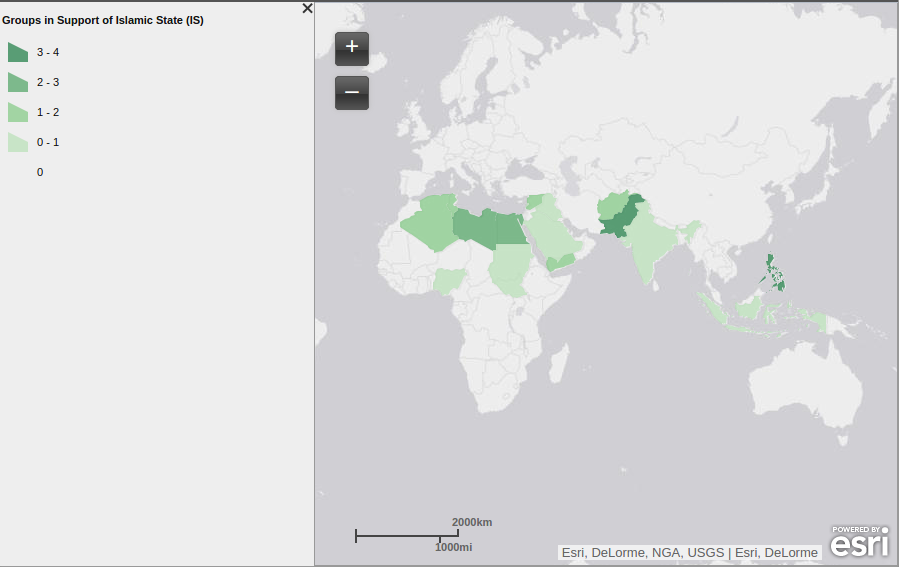
\includegraphics[scale=0.4]{./figures/affmap.png}
   \caption{Map of countries with ISIL affiliates \cite{IntelCenter2015}. }
     \label{fig:affmap}
\end{figure}



When considering ISIL's nuclear ambitions, one country not currently entangled in the ISIL conflict must be considered: North Korea.  In the past, North Korea has shown a willingness to export nuclear technology \cite{Wit2013}.  Some have argued the test of an uranium device in 2013 was an advertisement to the world that it could produce excess nuclear weapons that may be available for sale \cite{Allison2013}.  Currently, there is no known relationship between ISIL and North Korea.  However, given the unpredictability of the North Korean regime, coupled with the fact that there are operatives throughout ISIL controlled territory that would have North Korean contacts due to the prior Syrian - North Korean nuclear collaborations, any attempt to stop ISIL from obtaining a nuclear weapon needs to account for this potential pathway.   


Finally, it is important to consider the non-organizationally aligned support that ISIL receives in the form of foreign fighters.  The flow of these foreign fighters has dwarfed the influx associated with previous calls to Jihad, such as Afghanistan in the 1980s \cite{Barrett2014}.  These fighters come from all over the world as shown in \autoref{fig:enablers}, and they bring a diverse background and skill set with them.  Although no comprehensive list has been established in the open literature about the skills brought to ISIL via foreign fighters, it is likely that some of the foreign fighters possess skills necessarily to develop, fabricate, and assemble components of a nuclear weapon. 

\begin{figure}
 \centering
 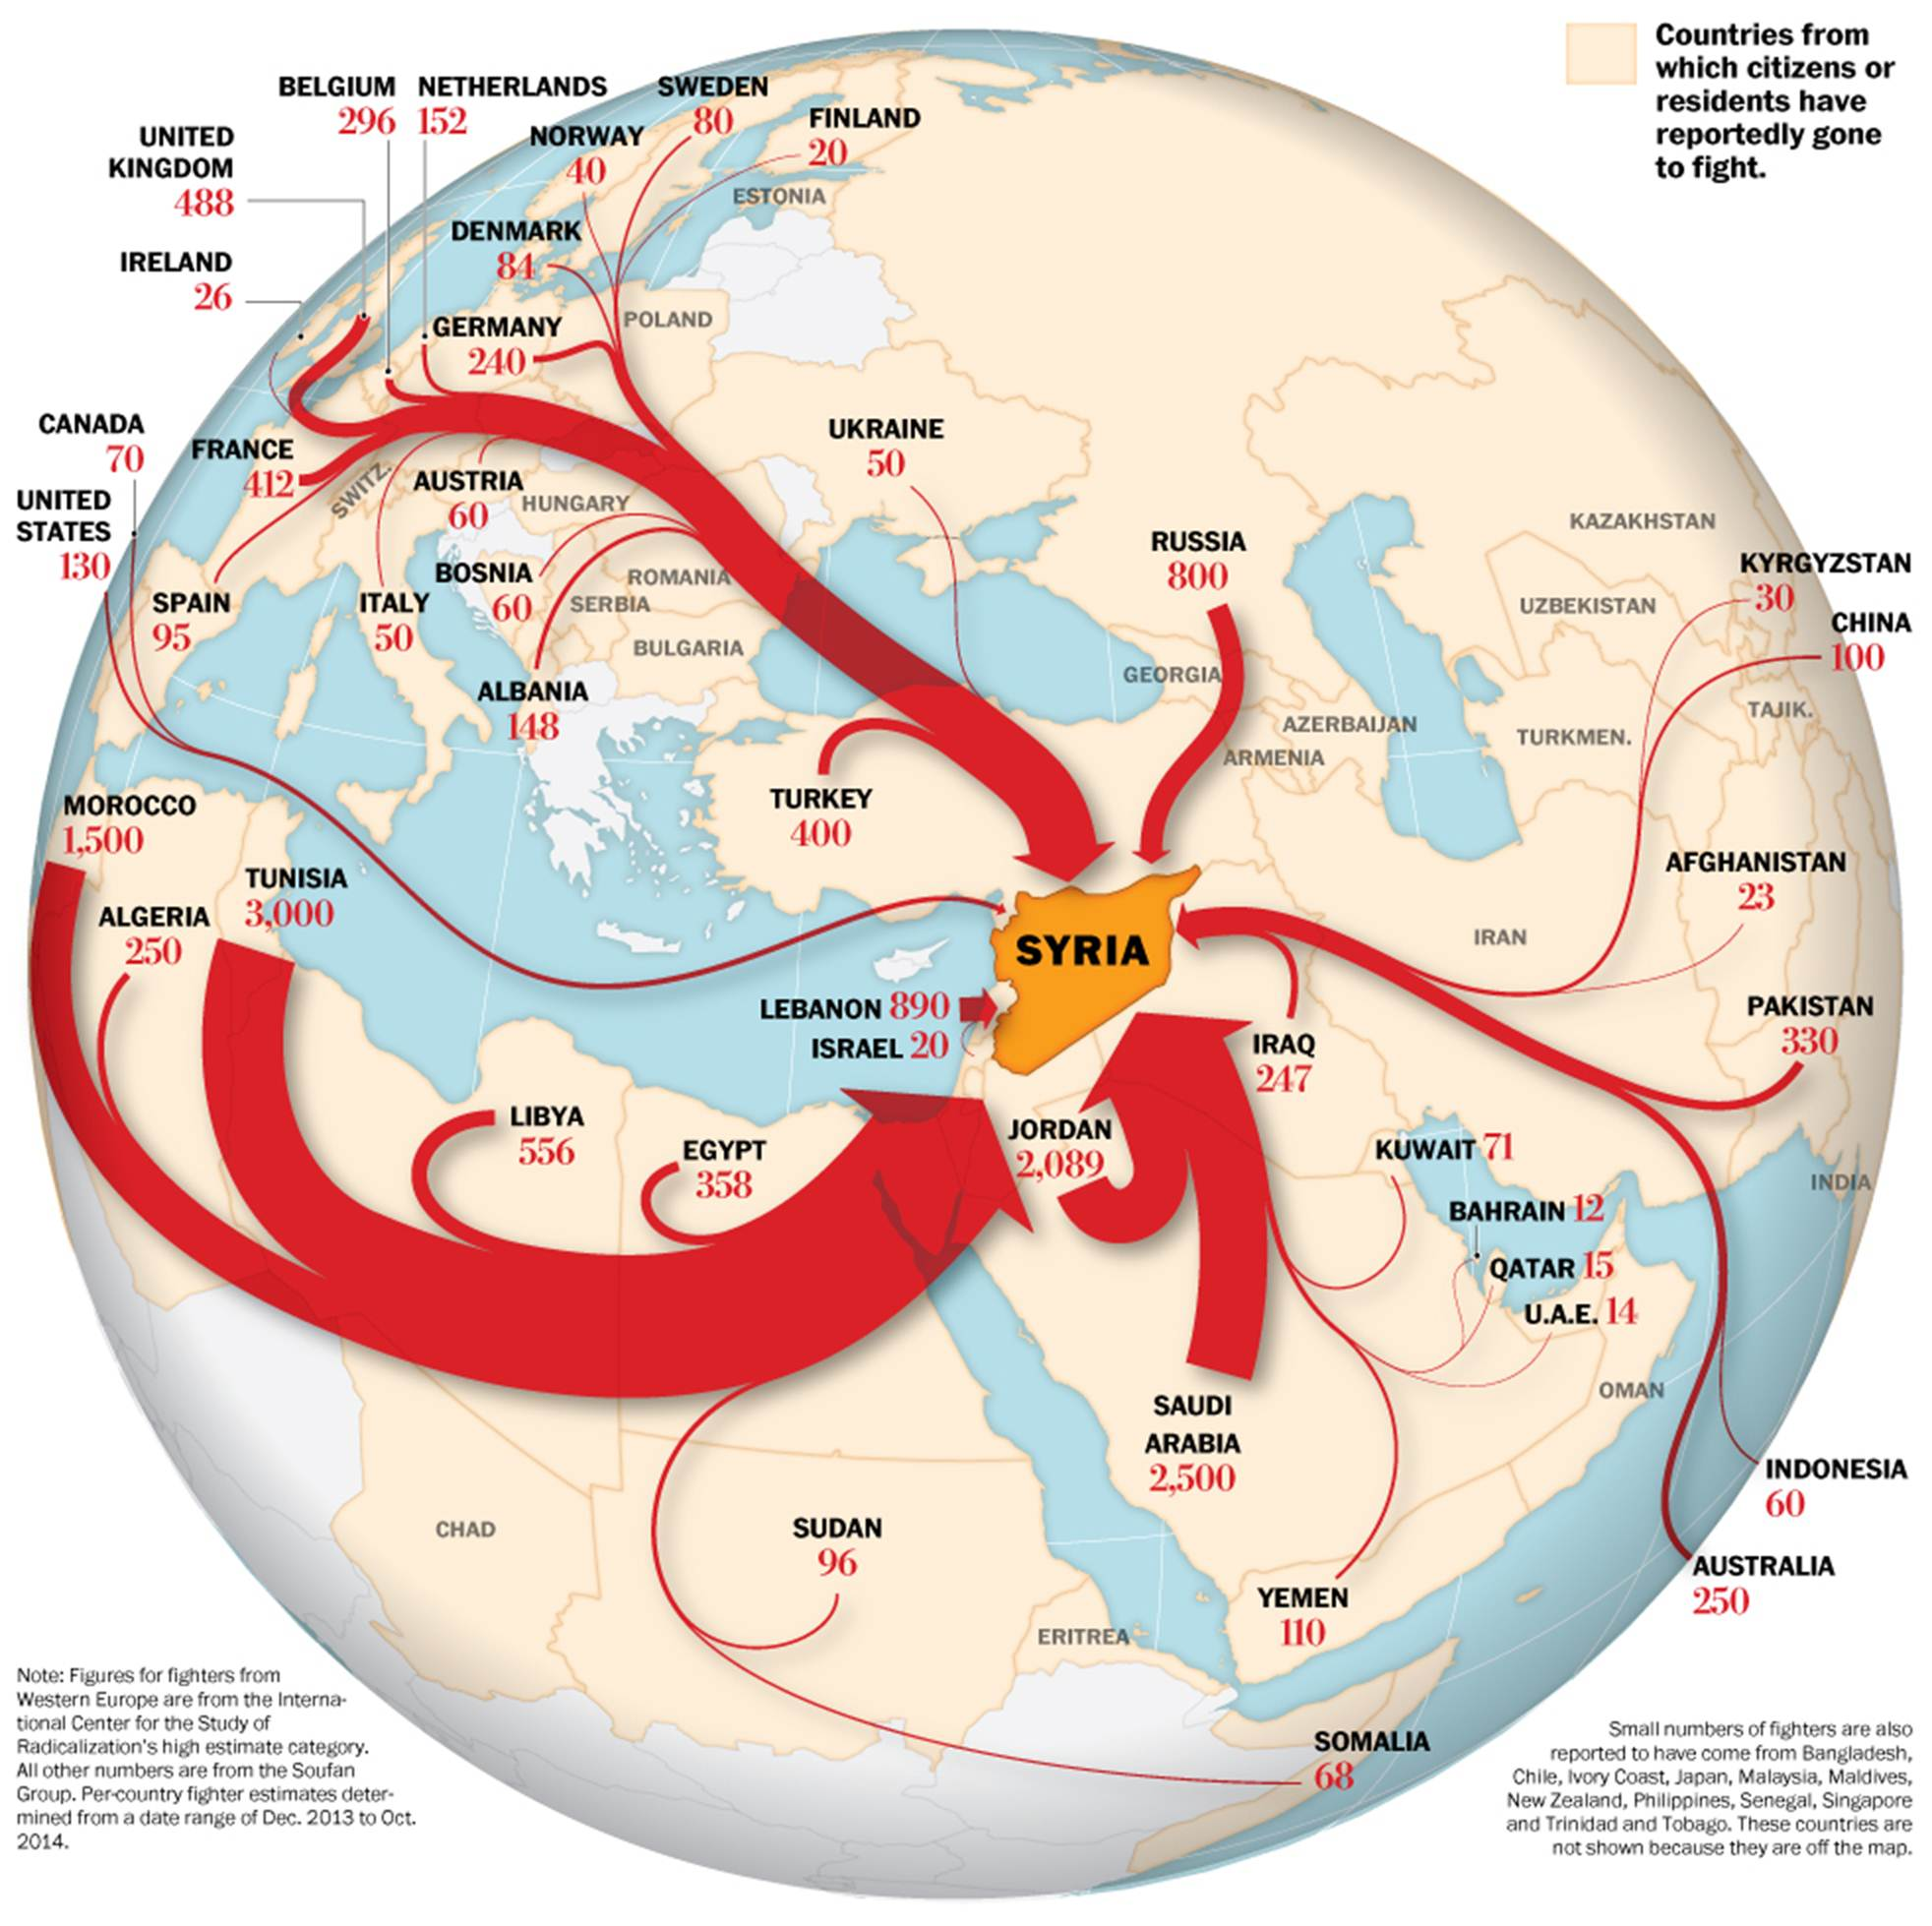
\includegraphics[scale=0.6]{./figures/enablers.jpg}
   \caption{Flow of foreign fighters into Syria \cite{Thorp2014}. }
     \label{fig:enablers}
\end{figure}







\chapter{Problem Definition}

\section{The Threat of an ISIL  Nuclear Weapon}

The threat of  nuclear weapon states is not a novel thought. Being the first and only nation to use a nuclear weapon against an enemy, the United States has feared a nuclear threat ever since weaponized nuclear technology became possible. Shortly after, the Soviet Union acquired nuclear weapons, marking the onset of the nuclear standoff during the Cold War.   Fortunately, through deterrence based on game theory against a rational adversary, not a single shot was fired between the U.S. and the USSR for approximately 44 years, until the conflict was alleviated. Since then, the nuclear threat has spread to many nations, including, most recently, Iran. 

The Iranian nuclear program has been called \enquote{the most vexing foreign policy challenge confronting the Obama administration}, and it is quite possibly the most difficult foreign policy challenge that the world has seen in many years \cite{Edelman2011}. Others have argued that Iran, as a large nation with much to lose, will develop the caution and restraint that is typically incurred by nuclear weapons development. This chain of events: weapons development, fear on a global scale, effective deterrence, and eventual restraint, has always been the crux of global nuclear weapons security. 

The world has not yet seen a nuclear capable entity    that is not sufficiently deterred by the threat of their own destruction. This is what makes ISIL a case of unique consideration. ISIL cannot be bundled into either the category of nations with inherent fear of self-destruction or the category of non-state actors with insufficient resources. They have continued to prove themselves as an organized and intelligent group that can continue to surprise the world with their capabilities. Their radically extremist ideology, vast independent wealth, powerful military, and pure ferocity set them apart from the organizations with whom the U.S. has historically dealt  \cite{bach2015isis}. 

The probability of ISIL acquiring nuclear weapons technologies and weapons is very low, so low, in fact, that this threat has been played down, with some dismissing the idea of an indigenous ISIL nuclear enrichment program as \enquote{impossible} \cite{AlexanderSmith2014,Cirincione2014}. The probability of ISIL obtaining a nuclear weapon may be incredibly small. However, risk is defined by both the probability of an occurrence as well as its potential consequences, which could be unfathomable \cite{ONeill1997}. Further, evidence  has  been reported  of ISIL  moving to obtain special nuclear material \cite{AlexanderSmith2014}. When it comes to nuclear weapons, the world cannot afford to be  surprised by ISIL. 

These low-probability, high-consequence events and any potential preventative policies are incredibly important to thoroughly analyze. For this reason, this report will focus on policies that could be implemented to prevent ISIL from gaining access to nuclear weapons technology and materials. Bernard Brodie said it best in Wizards of Armageddon: \enquote{nuclear war is unthinkable but not impossible, and therefore we must think about it} \cite{kaplan1991wizards}.





\section{Report Focus \& Framework}

This  report will evaluate and discuss the ability of  ISIL to engage in nuclear terrorism, so as to inform a policy statement to be enforced by the U.S.. This report considers the capability and resources of other sovereign powers and terrorist organizations when those may benefit ISIL. This policy statement details an organized response to any steps ISIL may make towards the deployment of a device containing special nuclear material (SNM). It stops short of a larger policy directed towards  the Administration's goal to degrade and ultimately destroy ISIL. 

The scope of this  report is limited to the materials, signatures, and means of detection for those signatures, in all phases during the development and delivery of a nuclear device. A brief summary of the relevant material and technology involved in the production and detection of SNM and nuclear weapons is presented here, to provide the reader an understanding of the relevant material involved in formulating a response policy for this scenario. This information was used to model all potential pathways by which ISIL could obtain a nuclear weapon. Appropriate policies for breaking the links in this pathway were developed leveraging existing policies, and recommendations were proposed for eliminating the threat of a nuclear capable ISIL.

This  report is directed towards the immediate response to development of the nuclear capabilities of ISIL, and does not consider the consequences which might result if ISIL were to evolve into a permanent state. This  time scale greatly reduces the possibility that ISIL possesses the infrastructure necessary to produce SNM or to assemble such material into a functioning warhead, unless they capture territory containing existing infrastructure. Due to the extreme sophistication in the triggering device, the development of thermonuclear weapons is very unlikely in the time window considered. Rather, emphasis is placed on diverting existing SNM from existing global stockpiles.

It must be considered that ISIL may orchestrate the delivery and detonation of a fission weapon or RDD without any of the material or components passing through territory which is directly controlled by ISIL. In this scenario, the search for SNM is a global concern, and the problem of detection and interception of such weapons or the orders to carry out such attacks is one which the international community must work together to address. 



\section{Limitations \& Assumptions of this Report}


This report and policy recommendation covers a sensitive and poorly understood subject: ISIL and the possibility of their acquisition of nuclear materials, or in the worst case, weapons of mass destruction (WMD). The combination of unknowns in this situation with the limited abilities and experience of the authors results in several limitations:

\begin{itemize}
  \item The principle limitation is ISIL themselves and the broad lack of information and deep understanding of their goals and the methods they are willing to employ.
  \item The authors have no access to classified information and therefore are not privy to the most up-to-date information on current international strategies and capabilities of all parties involved in the following discussion and recommendations.
  \item As a whole, the authors have very limited experience in this field. This is not a complaint on the authors' part, but must be understood and accepted to understand the biases and limitations of this report.
  \item Per the definition of this assignment, the authors  limited  their analysis and discussion to the scenario of ISIL attempting to acquire WMD; post-acquisition will be touched on briefly but should be analyzed in depth in a future report and policy recommendation.
\end{itemize}


These limitations are important to understand before analysis and discussion can be had and policy recommendations can be made. To move forward, several assumptions are made:

\begin{itemize}
  \item The United States is interested in stopping ISIL from acquiring a nuclear weapon and is willing to act decisively on this decision.
  \item Due to the nature of this threat, it is assumed that the U.S. will initiate policies and measures to prevent ISIL acquisition of a nuclear weapon; international support will be leveraged as appropriate.
  \item ISIL does want to acquire WMD and will act decisively on this desire.
  \item It is assumed that this policy applies only to the immediate future, and that if ISIL were to last for a longer time frame, more traditional state non-proliferation activities could take place.
  \item All other assumptions are more specific and detailed and will be discussed in further depth throughout this report.
\end{itemize}



This policy recommendation is oriented primarily towards responding and preventing ISIL nuclear capabilities. The scope encompasses strategic communication within the intelligence community as well as among the U.S. and potential countries and international entities and military capability. In the interest of time, this recommendation will not consider collaboration on information gathering or post-detonation. The following policy initiative will focus on developing an integrated intelligence strategy. 

\section{Problem Scoping}

This report was completed as a part of a graduate level Nuclear Security Policy course at the Goldman School of Public Policy and the Nuclear Engineering Department at the University of California, Berkeley. The class of approximately 20, including policy students and nuclear engineering students, was tasked with developing a policy recommendation for preventing ISIL from obtaining any nuclear capabilities.

As this is only a semester long project, there were great restraints on time and therefore scope. This report focuses solely on the paths to ISIL obtaining a nuclear capability. Of course, the fundamental way to preventing this would be to defeat ISIL in its entirety. However, given that the overall destruction of ISIL is a larger administration goal and is therefore being addressed by many other groups, our report focuses solely on nuclear capabilities. 









\chapter{Nuclear Weapons Primer}


This section is meant to serve as a basic guide to technical concepts necessary for understanding nuclear weapons. Although the content has been distilled to the most fundamental information and is deliberately simplified, it is critical to understanding the scientific context of nuclear weapons \cite{Prussin2014}. For flow of this report, the Nuclear Weapons Primer has been broken into 4 appendices: \autoref{app:glossary}, \autoref{app:physics}, \autoref{app:app_fuel_cycle}, and \autoref{app:weapons}.





A glossary of much of the nuclear-related terminology used in this paper may be found summarized in  \autoref{app:glossary}.


\section{Basic Nuclear Physics \& Definitions} 


\autoref{app:physics}  covers the basic nuclear physics needed to understand the functioning of a a nuclear weapon. It covers topics such as nuclear structure, criticality, fission, fusion, and energy release, all of which are key to framing the development of a nuclear weapon. Additionally, it covers radioactive decay, radiation interactions with matter, and biological effects of radiation, useful for understanding the consequences of successful detonation of nuclear weapons or RDDs. These concepts and definitions will be used throughout the report to explain and formulate technical and policy solutions to eliminate pathways for ISIL acquisition of a nuclear weapon.






\section{Fuel Cycle} \label{sec:fuel_cycle}


\autoref{app:app_fuel_cycle}  covers the basics of a nuclear fuel cycle necessary for both civilian and military uses of nuclear energy. The focus is on technologies and capabilities required to develop an indigenous nuclear weapons program. The Appendix addresses both the plutonium and uranium fuel cycles, and compares differences between the two. Any pathway to obtaining a nuclear weapon (other than theft or purchase of a complete nuclear weapon) will require one or more of the capabilities outlined in \autoref{app:app_fuel_cycle}.





\section{Weapons of Interest}


\autoref{app:weapons}  covers the basic categories of weapons enabled by nuclear materials: RDDs, fission weapons, and thermonuclear weapons. This Appendix builds on the concepts outlined in \autoref{app:physics} and \autoref{app:app_fuel_cycle}. Any ISIL pursuit of nuclear weapons or nuclear technology would ultimately result in the development of one of these three types of weapons.





\chapter{Enabling Capabilities }

\section{Intelligence }

% \subsection{Introduction}

The IC consists of sixteen distinct organizations managed by the Office of the Director of National Intelligence (ODNI) as depicted in \autoref{fig:structure_infographic}. These distinct organizations with divergent and overlapping capabilities, interests, and charters, can make a coordinated assessment of a dynamic threat like ISIL difficult. An overview of the IC and intelligence collected is provided in \autoref{app:intel}. Similar to the intelligence community (IC) reorganization following the 9/11 attacks and recommendations of the 9/11 Commission, the current threat of ISIL provides an opportunity for the IC to adapt to a dynamic threat environment and improve upon the weaknesses in IC structure and capabilities \cite{Kean2004}. Central to the U.S ability to deter ISIL from acquisitions of nuclear materials is an effective intelligence strategy to identify threats and guide response actions. 

\begin{figure}
 \centering
 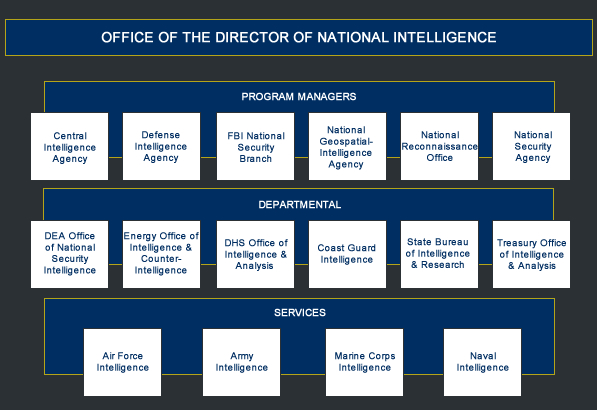
\includegraphics[trim = 0cm 0cm 0cm 0cm, clip,scale=0.7]{./figures/structure_infographic.jpg}
   \caption{Structure of the Office of the Director of National Intelligence \cite{OfficeoftheDirectorofNationalIntelligence}}
     \label{fig:structure_infographic}
\end{figure}

A basic assumption in our policy initiative is the ability of the IC to gather information through the use of radar, traditional and covert human sources, satellites, aircrafts, and ship signals \cite{Richelson2011}. This yields knowledge about the key primary, secondary and tertiary players involved, insight into the ideology and organization of ISIL, entities that might be providing it with economic or military aid, and operational details for the employment of a nuclear weapon.

From the U.S. perspective, 9/11 serves as a case study to understand the shortcomings of IC, subsequent recommended changes, and possible shortcomings facing the IC with respect to ISIL. The 9/11 Report found that there are cultural and organizational factors that hinder strategic communication between U.S intelligence agencies (See \autoref{app:partners} for a discussion on strategic communication on the international level, which also applies at the inter-agency level).  Prior to 9/11, U.S intelligence agencies operated in a culture dominated by \enquote{need-to-know}, which implied that organizations were given discretion in sharing data \cite{McConnell2008}. In the context of a dynamic ISIL threat, this means that agencies often have static analyses formed from an incomplete picture and lacking a competing analysis derived from the same data. The divisions between individual agencies render them incapable of accessing, prioritizing, translating, analyzing, and relaying the information for the policymakers to respond to in a timely manner. As a result, information flow is hindered by each agency's networks and databases lacking protocols to interact with other agencies' networks and databases.  Organizational inertia, standard operating procedures, and guidelines hinder the ability to change or implement new ideas. For example, the CIA's culture of risk aversion in the 1990s was detrimental to its intelligence capabilities and prevented them from properly assessing and taking action against the rising threat of terrorism \cite{Zegart2005}.

The situation is only complicated when considering international intelligence agencies and the sharing of data. To simplify the problem, the factors considered in determining the level of cooperation and the nature of an intelligence partnership between U.S. and other countries were distilled down to the historical relationships between both parties, the country's relationship to ISIL, its military and intelligence capability, and its vulnerability and geographical proximity to ISIL. The role of international entities is gauged by the organization's functions, credibility, and past success in relaying information and promptly responding to crises.  These factors are further described in \autoref{app:intel}. 

Using the guidance in \autoref{app:intel}, a framework can be developed for information exchange between countries: 

\begin{itemize}
  \item \textbf{Level 1:} U.S. should install open information sharing with the countries in category one. During WWII, U.S. and Great Britain had joint research of the atomic bomb. This cooperation can be repeated for actions against ISIL.
  \item \textbf{Level 2:} Information sharing with category two countries should be limited to low and medium security information (see \autoref{app:intel} for further description).  
  \item \textbf{Level 3:} The U.S. should consider to have limited information sharing of low importance security information with category three countries.  
\end{itemize}

Several international organizations and treaties are in place to facilitate communication flow and prevent the spread of nuclear weapons and technology (see \autoref{app:partners}).  However, communication in these organizations organization can be a challenge, and most of the current infrastructure is designed towards state actors, not the current ISIL threat.  Although not a specific alliance against ISIL or nuclear terrorism, the five eyes agreement (see \autoref{app:intel}) can provide valuable intelligence on possible nuclear activities that ISIL may engage. This group is stable, efficient, and more nimble in intelligence collaboration than the existing international non-proliferation structure.  

\section{Military Capability}




More than 60 countries have joined the \enquote{global coalition to degrade and defeat ISIL} \cite{Drennan2014}. The member countries can choose their method and level of participation. Saudi Arabia trains and equips Syrian opposition forces. Jordan's key role will be intelligence acquiring and sharing. Germany, France, and the United Kingdom are conducting airstrikes. 

The number of countries in the coalition is growing with Obama's campaign, but the bar for inclusion is fairly low. While many countries have committed military capabilities to combating ISIL, some countries join the coalition by merely declaring their intent to contribute. All these member countries don't share the same understanding of whom the real enemy is - ISIL or the Syrian regime led by President Bashar al-Assad. For example, Turkey has urged the coalition to topple the Assad regime as a condition to provide its air bases to carry out attacks against ISIL. 

% 
% \subsection{????? I don't know what to do with this section.  It covers several area, makes unsubstantiated claims, and doesn't really coherently address the coalition or military capabilities.  I think this needs rewritten and focused.  Statements such as "the country [UK] is extra vulnerable to terrorist attacks on its nuclear installations" needs a reference and doesn't belong in this section (Perhaps an Appendix and a reference to that appendix in section 2.3.  Topic of discussion is bracketed ?????}
% 
% \subsection{????? From here... ?????}
% The possibility of ISIL acquiring nuclear weapons means a stronger monitoring of nuclear-capable countries is needed. At the moment, only two handfuls of countries that have that capability. 
% 
% UK and France have been U.S.' allies even since the country launched its global fight against terrorism after the 9/11 incident. Hence, the U.S. can expect UK specifically to be its closest ally in preventing ISIL's nuclear terrorism effort. The two countries \enquote{special relationship} dated back to Churchillian era means that the U.S. can usually count on the UK for mutual support, especially considering ISIL's threats to the country is very high. UK has been ISIL's main target for terrorist attacks, and given UK's nuclear capability, the country is extra vulnerable to terrorist attacks on any of its nuclear installations. So far, UK has joined U.S.-led coalition against ISIL, nevertheless, prospect for bilateral cooperation between the two countries cannot be disregarded.
% 
% Meanwhile, France is U.S.' oldest ally and relationship remains active and friendly. France supported U.S. in various issues, however, France was skeptical when U.S. invaded Iraq after the 9/11 incident. ISIL has also posed great threats to France (being a successful nuclear energy producer and all), France can be vulnerable to attacks on its nuclear energy facilities as well as its possession of nuclear weapons stocks. France is also among ISIL's main recruitments considering France high marginalized and discontented Muslim populations. France's high ISIL threats and vulnerabilities made the country a good collaborator in effectively fighting ISIL.
% 
% Nuclear capabilities in the hand of weak or unstable government give opportunity for ISIL to acquire nuclear capabilities. Nuclear capabilities of Pakistan and its weak governance as well as security vulnerabilities is of concern to the U.S.. Looking at U.S.-Pakistan relationship, it has its ups and down. Over the decades, Pakistan has been a great ally to the U.S., but there are a few instance where the two countries were in disagreement. U.S. viewed Pakistan as its ally and threat in the country's global war on terror, in which Pakistan is seen as the \enquote{weakest link} as it continue to fail in containing act of terrorism going on in its own country. U.S. need to prop Pakistan and reduce the country's vulnerabilities of ISIL penetrations and the possibility of ISIL acquiring Pakistan's nuclear weapons.
% 
% India is also another country with nuclear weapon capability, and is mostly on the \enquote{other side} of U.S.' security policies. India, together with Russia was among the pioneers of Non-Aligned Movement (NAM), in which views on security issues tend to be divergent with the U.S.. However, as of recently, the U.S. and India have set up \enquote{global strategic partnership}, based on shared democratic values and increasing convergence of interests on bilateral, regional and global issues; key recent developments in the relationship include the rapid growth of India's economy and bilateral trade, the close links between the Indian and American computer and Internet industries, a geopolitical coalition to balance the rise of China, the weakening of U.S.-Pakistan relations, among others. U.S. has cooperated with India in area of civil nuclear, and this can be expanded to development of nuclear security hopefully in the future. However, unlike Pakistan, India believed ISIL's threats as periphery issue to the country.
% 
% In analyzing Russia as a possible bilateral partner, the two country has had strained relationship, increasingly since the economic sanctions imposed by the U.S. to Russia. Dispute between the two countries have centered on power struggle for new world order, and recently exacerbated by Russia's annexation of Crimea. The two countries have been historical rival and the Cold War has proven to be one of the expansive and stretched out power struggle between the two. However, both countries realized and agreed to maintain dialogue in several areas including terrorism. Being misaligned with Russia on ISIL and nuclear terrorism issue could be serious mistakes as Russia's nuclear capability, if not protected and are allowed to be shared in the wrong hand, could have grave catastrophic impact to global security environment.
% 
% China, another U.S.' partner and rival at times, also have nuclear capabilities. China and the U.S. has close partnership particularly in economic sector, two-way trade between the two countries is over U.S.\$590 billion in 2014 alone. Chinese Muslim Uyghur militants have been associated with ISIL and efforts to undertake terrorist attacks in China. This strengthen the need for collaboration between China and U.S.; to ensure any ISIL activities can be contained in China and the country's nuclear weapons is protected from any probability of ISIL acquiring them.
% 
% U.S. considered North Korea as grave threats and this can be further exacerbated if North Korea is presented with the opportunity to work with ISIL. The prospect of North Korea selling their nuclear weapons and missiles to ISIL cannot be discounted. However, the possibility of U.S. and North Korea to cooperate in hampering this issue is not viable. The U.S. need to come up with initiatives to solve this problem.
% 
% Iran and U.S. shared a common enemy factor in terms of ISIL. As the nuclear talks between the two countries are being hashed out, both countries have committed on fighting ISIL together. This can be a good opportunity for U.S. to combat ISIL more effectively as U.S. cannot disregard Iran's influence and role in Iraq's security landscape and their fight against ISIL.
% Meanwhile, collaborating with Israel is considered a gray area and not clear-cut as it seems. Israel has been known to voice their support of ISIL, keeping in line with ISIL's common enemy with Israel i.e. Iran. As U.S. and Israel have been a strong ally in the Middle East region, this fact presented a conundrum to the U.S..
% 
% The U.S. may find other allies in the Middle East region, however, the region is deeply divided in their positions against the ISIL. Although most Middle Eastern countries sees ISIL as a serious threat to the region and its people, some still supported ISIL, if not openly but explicitly. U.S. has worked closely with Jordan, with the U.S. creating a U.S.\$5 billion counterterrorism partnership fund with Jordan and other countries (Libya, Lebanon, Syria) that are considered on the \enquote{frontlines} of U.S.' fights against ISIL.
% 
% The U.S. can find allies in European countries as well, as the region is facing \enquote{recruitment} threats from ISIL. Thousands of Europeans have been recruited by ISIL to fight jihad cause in ISIL's territories. ISIL is also setting up bases in a number of European countries, expanding its influence beyond the Middle East region. The U.S. can identify these countries and create cooperation efforts in order to effectively eliminate ISIL.
% 
% \subsection{????? ...to here. ?????}


\section{Pre-Detonation Nuclear Forensics}

Following the interception of SNM or weapon components, careful analysis of the composition, material structure, and relative sophistication of the physics package will allow forensic investigators to estimate the age of the device, the techniques which were utilized in order to create the physics package, and the most probable country of origin \cite{Glaser2008}. In the U.S., a number of organizations would be involved in these assessments. The National Technical Nuclear Forensics Center (NTNFC) is responsible for ensuring the nation's nuclear forensics capability.  The NTNFC is supported by the Department of Homeland Security (DHS), Department of Justice (DoJ), Federal Bureau of Investigation (FBI), Department of Defense (DoD), Department of Energy (DoE), Department of State (DoS), and the Office of the Director of National Intelligence  \cite{DepartmentOfHomelandSecurit}. 

The age of the physics package is determined from the composition. Because SNM is, itself, radioactive, a small amount of mass is converted to heat and radiates off. It is possible to approximate the change in mass by estimating the age of the original physics package based on the apparent design of the weapon; this change in mass correlates to the age of the device since the physics package was created \cite{Inn2013}. See \autoref{sec:intro_active_interrogation}, \enquote{Introduction to Active Interrogation,} in \autoref{app:tech} for a description of the technical means of estimating the composition of SNM. The country of origin for Uranium-based weapons may be narrowed down based on the initial enrichment of the material \cite{Defense1998}. The facility of origin may be determined in Plutonium-based designs based on the ratio of isotopes present, as shown in \autoref{fig:pu_signatures}.

\begin{figure}
 \centering
 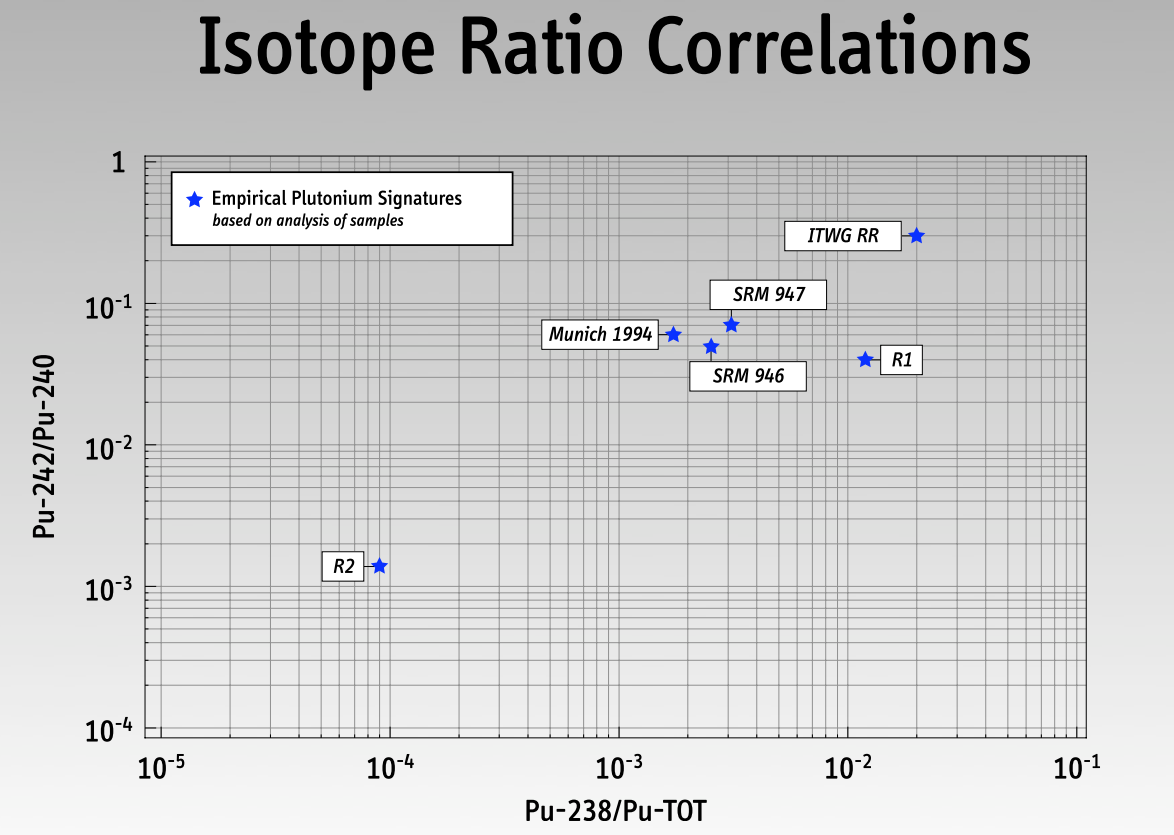
\includegraphics[trim = 0cm 0cm 0cm 0cm, clip,scale=0.3]{./figures/pu_signatures.png}
   \caption{The expected and measured ratio of isotopes of Plutonium, listed by facility of origin \cite{B412922A}.}
     \label{fig:pu_signatures}
\end{figure}


The manufacturing techniques could be determined from micro-analytical techniques which measure the oxidation state and crystalline form of the special nuclear material; however, the results of such studies are often inconclusive and may require up to a few weeks for a complete analysis \cite{Drell1995}. Additional details on the nature and implementation of pre-detonation forensics are listed in reference \cite{Doyle2011}. 




\section{Post-Detonation Nuclear Forensics} \label{sec:post_det_forensics}


The goal of post detonation forensics is to determine the design, composition, and origin of a nuclear weapon. To assist in the attribution process, there exists a distributed network of monitoring stations which measure different signals which would confirm the occurrence and characteristics of a nuclear detonation. These stations include: over 170 seismic monitoring devices, six underwater (hydroacoustic) and 5 land systems which monitor sound waves, and 60 surface stations which measure infrasound (ultra-low-frequency) \cite{Lane2012}. The location of detonation and the yield of the nuclear device may be estimated from an analysis of these signals. In the hours and days that follow detonation, measurements of the radionuclide composition near the blast zone and in the plume of gas and dust released into the upper atmosphere allow conclusions to be drawn concerning the efficiency of the device, the weight of the fuel (i.e. the level of sophistication), whether the fuel was plutonium or uranium, how the fuel was created, and whether or not DT fusion occurred (based on the known cross-sections of 14 MeV neutrons with the surrounding environment) \cite{Davis2011}. Additionally, there exists a vast orbital infrastructure which monitor for optical, X-ray, gamma-ray, and neutron emission characteristic of nuclear detonations; the exact capabilities of these systems is classified \cite{1446400}. 

\subsection{Data Processing \& Response Time}


If nuclear material is intercepted before detonation, an analysis of the enrichment and contaminants may be achieved at the National Labs (Oak Ridge, Los Alamos). On the scale of weeks to months, it is possible to discern the age of the material post fabrication by analyzing the micro-structure, activity, and isotopic composition. Immediately following detonation, the timescale of analysis relies on how quickly radiation monitoring equipment may be delivered to the blast site and how quickly samples are gathered and shipped back to one of 16 radiological facilities equipped to perform nuclear forensics \cite{1446400}. Airplanes capable of sampling large volumes of the dust and gas (Xenon) in the plume generated by the detonation must be performed within 1-2 days of the detonation and may indicate the composition, efficiency, and sophistication of the device. Analysis of materials taken from the ground near the detonation point will take 1-2 weeks to analyze and will confirm and refine the findings of atmospheric monitoring. The identification of the origin of the weapon will depend largely on what is presently known about the yield, sophistication, and efficiency of weapons in global stockpiles. What is exactly known of the capabilities of weapons designed outside of the United States is classified \cite{Glasstone_1964}. Given quick access to the nuclear blast site and a somewhat thorough understanding of the nuclear capabilities of other sovereign powers, the technical analysis of the origin and design of a nuclear blast would be available within 3-10 days, depending on the availability of data. Ongoing research is aimed at developing LIBS technologies which may reduce the nuclear forensics timeline with rapid (\textless 15 hours) debris dissolutions techniques, or techniques which do not require the dissolution of collected debris \cite{Condron}. 


\section{Detection Technologies}

The National Nuclear Security Administration (NNSA) collaborates the efforts of the Defense Threat Reduction Agency (DTRA), the U.S. National Laboratories, and other federal agencies to locate and identify special nuclear material \cite{NationalNuclearSecurityAdministration}. Detection of radioisotopes requires an understanding of the type and energy of radiation and the material response in detection systems (see \autoref{app:tech} for a discussion of passive and active detection of the radioactive materials employed in fission weapon and a radiation dispersal device). As a general overview, the success of the detection of radioactive materials relies on specialized equipment, minimizing the distance to the material, collection time to improve statistics and resolve a signal above background, and, in some circumstances, utilizing reach back for specialized interpretation of the results.


Presumably, the clandestine transport of SNM will be shielded to reduce or eliminate the apparent signal available to detection systems outside the transport container. The cost of search and seizure of every container across international borders is prohibitively expensive. The alternative searching method favored by the NNSA is standoff, active interrogation, where an interrogating beam of neutrons or gamma rays is used to induce a high energy signal from radioactive materials hidden behind shielding. The application of active interrogation is only effective if a significant portion of traffic into each country is subject to search (see \autoref{app:tech}  for a discussion of the benefits and disadvantages of active interrogation). However, it is worth noting that active portal monitoring is expensive and would require years for systematic deployment, but passive monitoring stations could be employed more rapidly \cite{Grogan201362}. 

 
\subsection{Shielding of Radioactive Materials}  \label{sec:shielding_mat}


Of the radiation types mentioned (alpha, beta, and gamma), the gamma emitters are by far the farthest penetrating, most energetic, radioisotope emitters listed \cite{krane1987introductory}.  The shielding suggested will merely attenuate the energy levels of the gamma emissions, but in essence the emission passes through the shielding and continues on its travel through the medium. \autoref{fig:shielding_reqs} shows relative stopping distances in materials for given radiation types. 

\begin{figure}
 \centering
 
\includegraphics[trim = 0cm 0cm 0cm 0cm, clip,scale=0.5]{./figures/shielding_reqs.jpg}
   \caption{Schematic representation of the shielding requirements of alpha, beta, and gamma radiation \cite{Hallenbeck1994}. }
     \label{fig:shielding_reqs}
\end{figure}


Alphas, although very energetic upon initial release from the source, are very large particles in comparison to the surroundings.  It is more likely that the 2+ charged alpha ion will interact with matter than the other radiation types; even as depicted, a piece of paper is sufficient shielding material to attenuate alpha emissions \cite{krane1987introductory}. Thus, shielding SNM to prevent detection of its alpha signatures is unnecessary, as the air in between the SNM and a detector (more than a few cm away) would shield the alpha particles \cite{Cember2008}. 

To shield SNM against the more penetrating beta particles and neutrons, water, concrete, paraffin, high-density plastics, or boron-based materials (such as boron carbide or borosilicate glass) could be easily used \cite{Cember2008}. These would not only shield against passive detection of the SNM, but against neutron interrogation - based active detection methods as well, given a few feet of shielding \cite{Grogan201362}.

To shield SNM against gamma rays and X-rays, lead and concrete would be the most common choices of material \cite{Cember2008}.  These would not only shield against passive detection of the SNM, but against X-ray fluorescence - based active detection methods as well, given more than several inches of lead shielding \cite{PhysRevC.78.041601,Grogan201362,Bertozzi2005}.

Thus, the most  effective shielding to prevent passive or active detection of SNM would likely be a combination of layers of paraffin (preferably boron-impregnated) and lead.













\chapter{Policy Response}




\section{Overview} 

In attempting to prevent the acquisition of nuclear material, first and foremost the U.S. should continue this administration's declaratory policy: \enquote{our objective is clear: We will degrade, and ultimately destroy, ISIL through a comprehensive and sustained counterterrorism strategy} \cite{Hudson2014}.  The policy recommendations outlined below are meant to build on, not replace, the current efforts at defeating ISIL. Recommendations are listed in order of priority, based both on ease of implementation and effectiveness at preventing ISIL from obtaining a nuclear device. 


These recommendations were developed by modeling the steps ISIL would have to take to procure a nuclear device, from the inception of the idea, to staging and detonation. Each recommendation is meant to target a specific chain of this logic model, with the ultimate goal of destroying all paths ISIL may have to a nuclear device. The logic model is shown in \autoref{fig:logic_tree}, with different nodes highlighted to represent the level of risk to the U.S., with green cells being high risk, orange medium, and red low. \autoref{fig:policy_chart} shows a summary of the existing and recommended policies, and are expanded upon in the sections to follow. In \autoref{fig:policy_chart}, the targeted capability and pathway coloring scheme corresponds to the same coloring scheme used in \autoref{fig:logic_tree}. The proposed policies are colored by their chance of success in disrupting the particular pathway: green is high, orange is medium, and red is low.




\includepdf[angle=270, pagecommand={\thispagestyle{fancy2}\null\vfill\captionof{figure}{ISIL Logic Tree}\label{fig:logic_tree}}, scale=0.85]{./figures/NucSec_Logic_Model2.pdf}



\begin{landscape}

\begin{figure}[H]
 \centering
 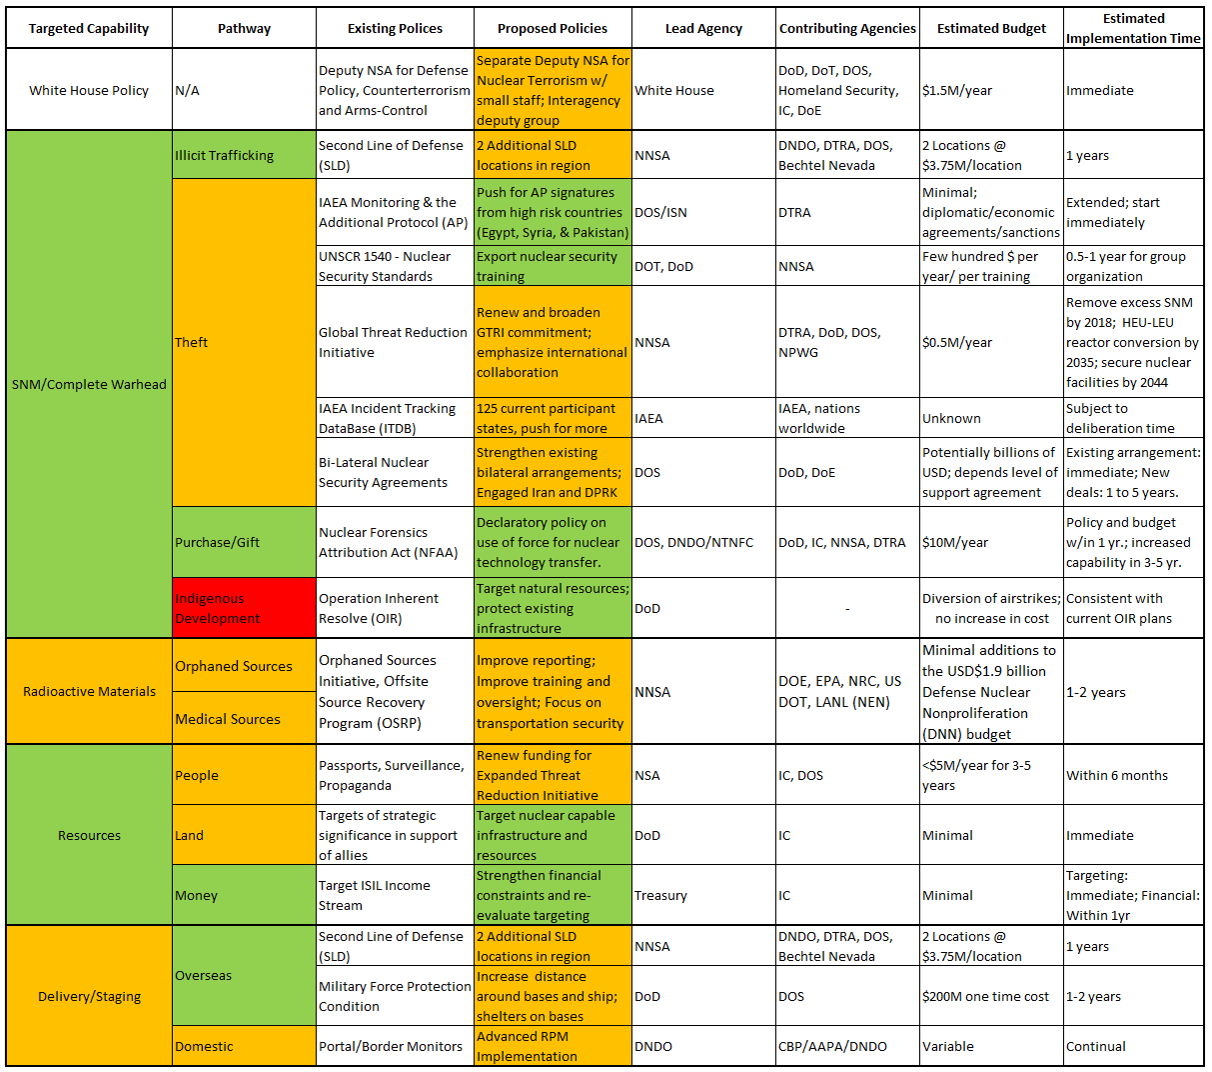
\includegraphics[trim = 0cm 0cm 0cm 0cm, clip,scale=0.52]{./figures/PolicyChart4.png}
   \caption{Summary of existing and proposed policies to combat ISIL acquisition of nuclear weapons.}
     \label{fig:policy_chart}
\end{figure}

\end{landscape}



\section{Coordinating Government Efforts to Counter Nuclear Terrorism}

\subsection{Putting Someone in Charge}

A key step for the United States in preventing ISIL acquisition and use of a nuclear device is to coordinate and organize the various initiatives across the government that are handling various pieces of this puzzle. In 2008, the authors of a Belfer Center report on preventing nuclear terrorism recommended that President Obama appoint a senior figure to a post in the National Security Council (suggesting this may be a new Deputy National Security Advisor) with the sole responsibility of waking up every morning and thinking about how to prevent a nuclear terrorist attack \cite{Bronner2008}. Since that time, President Obama created a new White House post called the White House Coordinator for Defense Policy, Countering Weapons of Mass Destruction, and Arms Control. The National Security Staff's former Senior Director for Europe, Liz Sherwood-Randall was promoted to that position \cite{Rogin2013}. While this is a step in the right direction, the arms-control role of this position is likely to consume much of Ms. Sherwood-Randall's time, forcing her to put some anti-nuclear terrorism initiatives on the backburner. For this reason, this report recommends that the White House:

\begin{itemize}
 \item Break out the countering nuclear terrorism aspect of the role of White House Coordinator for Defense Policy, Countering Weapons of Mass Destruction, and Arms Control, and create a new White House role within the National Security Council that deals exclusively with nuclear terrorism, preferable a Deputy National Security Advisor for countering nuclear terrorism. 
 \item Limit the responsibilities of this role to nuclear terrorism, leaving out nuclear weapons concerns as related to Pakistan, North Korea, and Iran, as well as arms-control. These concerns would dominate much of this person's time, detracting from the necessary focus on preventing nuclear terrorism.
 \item Fill this position with a senior figure who commands respect across cabinet departments, and is capable of speaking on behalf of the president.
\end{itemize}

This person would have full responsibility for coordinating and overseeing counter-nuclear terrorism efforts. Making this role a Deputy National Security Advisor would have the advantage of giving the role the authority to integrate policies across the Department of Defense, the Department of Energy, the State Department, the Intelligence community, Homeland Security, and law enforcement \cite{Bronner2008}. This person would also have a role working with the Office of Management and Budget (OMB) to ensure that all agency budgets are aligned with a comprehensive strategy. Additionally, the President can direct OMB to prepare a crosscut of departmental budgets to find all funds associated with preventing nuclear terrorism and put them under a single budget examiner \cite{Bronner2008}.

The above suggestions are consistent with the 2008 report from the Belfer Center. The report also emphasizes the importance of limiting the scope of this proposed role. In particular, this person should not be responsible to Pakistan, Iran, or North Korea, because these issues would take up all of this person's time \cite{Sharp2008}. This is the key problem with the current National Security Council role occupied by Ms. Sherwood-Randall - with arms control and broader counterterrorism efforts under her purview, there is still need for a senior official at this level in the White House dedicated exclusively to preventing nuclear terrorism. The full-time focus on nuclear terrorism will create an opportunity for addressing lower-level threats, as opposed to disproportionately planning for worst-case scenarios. A strategic operational plan put forward by this person can create obstacles to acquisition of nuclear weapons for terrorist groups by squeeze groups from all sides \cite{Levi2008,Ferguson2006}.  In doing this, this person may also call on collaboration from the National Counterterrorism Center.

Assuming that the White House institutionalizes this role as a Deputy National Security Advisor, the costs associated with this recommendation equal the salary and benefits of this person as well as a small staff. There will also be costs associated with the initiatives created by this person and other staff time that is devoted to those initiatives. Creating this role is an important step in crafting a strategic plan that integrates departmental efforts. The downside to this recommendation is that the efforts of this person are likely to be hampered by turf wars inherent in integrating departmental efforts; however, this difficulty can be mitigated by an approach that seeks to provide departments with a framework for evaluating and adjusting their efforts in the context of the broader effort, rather than mandating changes from the top down \cite{Levi2008}. This way, it promotes cross-agency relationships and personnel become better equipped at sharing and comparing methods of collecting and analyzing information.  Agencies should be less structured on rules and regulations and instead focus on how to best adapt to changing circumstances. A combination of minimal oversight and conflicting missions due the independent nature of these agencies \cite{Zegart2005} require that this person implement a uniformity of standards to decrease costs and simplify the flow of information. 


Finally, this person should have a small staff that will help him or her put into place a comprehensive, prioritized plan to combat nuclear terrorism. This person will drive the government-wide efforts to prevent ISIL acquisition and use of a nuclear device. 

\subsection{Creating an Interagency Group}

It will also be important for the White House to create a deputies committee focused on nuclear terrorism, led by the proposed Deputy Nuclear Security Advisor for Countering Nuclear Terrorism and including deputies with sole responsibility and departmental oversight of counter-nuclear terrorism from DoD, DoE, the State Department, Homeland Security, and law enforcement \cite{Bronner2008}.

Additionally, current efforts within departments remain split into various lower-level groups. In order to increase the effectiveness of department efforts and the implementation of the deputies committee, the White House should direct the Department of Energy, the Department of Defense, the State Department, and Homeland Security to have on official presiding over efforts to prevent nuclear terrorism. 

\subsection{Articulating Priorities}

Another White House priority should be to articulate the central importance of combating ISIL efforts to acquire and use nuclear weapons. Creating a new Deputy National Security Advisor position is the beginning of demonstrating counter-nuclear terrorism as a United States priority and broadcasting this commitment to the international community. 

In order to deal specifically with the ISIL threat, the White House should designate a focus on ISIL as a responsibility of the suggested Deputy National Security Advisor. The White House may also want to seek from Congress an appropriation to be available until expended on high-priority actions that will reduce the risk of nuclear theft and smuggling \cite{Bronner2008}. While articulating the request for the appropriation, the White House should focus on outlining the ISIL threat, and the ways in which the money could be spent that will cut down on the chances of ISIL acquiring a nuclear weapon - while reducing risk of other terrorist groups obtaining a nuclear weapon simultaneously. 

\subsection{Build International Consensus}

In addition to taking the actions outlined above, the United States should launch a global security campaign aimed at building consensus that steps must be taken to reduce the risk of nuclear terrorism, encouraging allies and other nuclear powers to create high-level positions (similar to the proposed Deputy National Security Advisor), and coordinating state efforts to combat nuclear terrorism \cite{Ferguson2006}. 





\section{Fundamental Efforts}


There are three approaches to disrupting ISIL operations that will be particularly important in ensuring that ISIL does not acquire a nuclear device:

\begin{itemize}
 \item Disrupt ISIL cash flow
 \item Restrict ISIL access to nuclear weapons experts
 \item Rollback ISIL territorial gains
\end{itemize}

\subsection{Disrupt Cash Flow}

\bfseries Targeted Capability: Resources 

Pathway: Money 

Existing Policy: \textcolor{red}{Target ISIL Income Stream}

Proposed Policy: \textcolor{red}{Strengthen financial constraints and re-evaluate targeting}  

Lead Agency: DoT

Contributing Agency: IC \normalfont


ISIL's principal source of cash flow comes from the control and sale of oil, which brings in about \$1 million a day. ISIL is also financed through kidnappings, extortion, criminal activities, and a small amount from external donations \cite{Lister2014}. ISIL employs roughly 30,000 fighters, including 19,000 foreign fighters from 90 different countries, paying them roughly \$350-\$500 a month. This comes out to \$10 million per month. ISIL also recruits fighters in the region by providing electricity and other services to local residents \cite{TheEditorialBoard2015}. A new report by the  Financial Action Task Force (FATF) finds that it is unclear whether ISIL's revenue collection will be sustainable over time, and that ISIL will have to gain more territory to remain financially viable \cite{TheEditorialBoard2015,Report2015}.

The Department of Treasury (DoT) has prepared a strategy to disrupt ISIL's revenue streams by targeting sanctions, cutting off cross-border oil smuggling, and refusing to pay ransoms for kidnappings \cite{Cohen2014}. In undermining the group's ability to generate revenue, these steps will also slow or halt ISIL's potential WMD acquisition process by reducing the funds available to ISIL to purchase a bomb or fissile material, create an indigenous capability, recruit nuclear scientists, or make territorial gains that could give them access to sensitive facilities. The DoT strategy is to:

\begin{enumerate}
 \item Disrupt revenue streams
 \item Restrict access to international financial systems
 \item Target leaders and supporters with sanctions
\end{enumerate}

We believe DoT's approach to degrading ISIL's financing is the most effective available route, and that disrupting finances through targeted sanctions remains a strength of the broader U.S. approach to ISIL. Our primary recommendation is that DoT continues with the path it has staked out to degrade ISIL finances. In addition to holding to the current playbook, we propose several small recommendations that may help to advance DoT's efforts:


\begin{itemize}
 \item The United States should evaluate the viability of phasing away from targeting oil fields for air strikes, and instead target ISIL's transportation and sale of oil, in order to preserve oil infrastructure for civilians in ISIL control areas, which we anticipate will weaken ISIL's recruiting efforts by mitigating anti-American sentiment \cite{Lister2014}.
 \item In aiding opposition groups in northern Syria, the United States should provide large quantities of diesel fuel and oil for generators in the areas controlled by these groups \cite{Lister2014}.
 \item The State Department and U.S. Embassies should continue to work with Kuwait and Qatar, along with other government in the region, to create and strengthen legislation that counters financing of ISIL's efforts \cite{Lister2014}.
 \item The State Department should provide incentives to the cyber security and reconnaissance and surveillance industry to continually provide the intelligence community with information about ISIL activities.
\end{itemize}




\subsubsection{Disrupt Revenue Streams}

DoT has stated that it will impose targeted sanctions on anyone who purchases ISIL oil. Additionally, DoT is working to identify middlemen, refiners, transporters, and everyone else in the supply chain \cite{Cohen2014}. Beyond sanctions, DoT is working to stem cross-border oil smuggling, in collaboration with others in the U.S. government as well as Turkish and Iraqi Kurdish authorities \cite{Cohen2014}.

Crippling ISIL oil revenue, however, is likely more complicated than it might seem. ISIL has been working to establish an internal market for their oil by providing cheap oil to the people in the territories they control, and by using it to fuel their own fleets \cite{Lister2014}. Some of the major U.S. airstrikes have targeted oil fields, but this also cuts off oil supplies for Syrian rebels and civilians in the region. This has been a central complaint of Syrian rebels, who lament that airstrikes disrupt oil supply to power generators and local facilities, allowing ISIL to pass the blame on to the United States. The United States should evaluate the viability of phasing away from targeting oil fields for strikes, and instead targeting ISIL's transportation and sale of oil. This approach may be made more viable by intelligence generated by DoT's efforts to identify everyone in the ISIL oil supply chain. In the meantime, the United States should provide large quantities of diesel fuel and oil for generators in opposition areas of northern Syria \cite{Lister2014}, in order to offset fuel and oil disruption due to U.S. targeting of oil fields. This would also diminish the demand for illegally-smuggled ISIL oil.

In the current oil market, diminished profits from selling oil may make ISIL more dependent on external donations. As need for this arises, it is important to focus now on these external sources. DoT has worked to choke-off key smuggling routes, and good work has been done in Saudi Arabia and UAE to crack down on ISIL oil sales there. However, while Kuwait and Qatar have passed legislation to counter financing of ISIL and other terrorist groups, both countries remain too permissive of ISIL oil sales and other forms of terrorist funding. More needs to be done by these states to enforce their newly passed laws against financing terrorism, and the United States should reach out to these states via the State department and U.S. embassies in order to make sure that these states are cracking down on terrorist funding. Diplomacy of this type promises mutual gains, since both Kuwait and Qatar have an interest in stopping ISIL, which has periodically targeted Qatar and its Ministry of Foreign Affairs \cite{Lister2014}.

Extortion and illicit taxation are large, internally sustainable methods of funding for ISIL. Before capturing Mosul, ISIL was already earning \$12 million a month in the city from these methods. A sophisticated ISIL taxation system has been created in on the main highway between Jordan and Baghdad that replaces the government's import tax by charging a reduced rate for goods transported into the capital. ISIL does this throughout Iraq and Syria, and ensures its survivability by gaining tax income while charging low rates to Sunni truckers and other Sunnis to curry favor. Truly eroding this source of funding means breaking ISIL's hold over the territory. This is highly unlikely to happen without sophisticated ground forces following up on the airstrikes. This will be discussed in greater depth in the section on rolling back ISIL's territorial gains \cite{Lister2014}.

Another source of ISIL funding is social media fundraising. The group has demonstrated the ability to engage in complex online fundraising activities; ISIL even uses \enquote{tiered} donations common to crowdfunding sites in which donors get various perks and special thank-you messages depending on their level of donation \cite{Report2015}. 


British Aerospace (\enquote{BAE}) systems and other surveillance and reconnaissance companies have mapped ISIL's social network by data mining to collect information from social media accounts linked to ISIL \cite{Tadjdeh2014}. These companies and others should be incentivized to continue to gather information on ISIL's efforts and to scour the Internet for threats, including identity and intellectual property theft. The State Department can support these efforts by providing incentives to the industry to provide the U.S. government with information about ISIL activities. A final recommendation is to put more of the government's own intelligence resources toward detecting ISIL social media fundraising efforts \cite{Report2015}.

\subsubsection{Restrict ISIL Access to International Financial Systems}

Operating entirely in cash is risky and cumbersome, and it will be important for ISIL to access the banking system in Syria, Iraq, and internationally. Access to the international banking system is also important for ISIL to fund external operations, including operatives who may be tasked with attacking the U.S. homeland. DoT is aiming to prevent ISIL from using bank branches in the territory where ISIL operates, as well as the international banking system as a whole \cite{Cohen2014}. The private sector is also important in these efforts. The Bank Secrecy Act allows private companies to give DoT insight into financial activity in areas where ISIL operates \cite{Cohen2014}. DoT efforts in this area are strong and should continue.

\subsubsection{Target ISIL Leaders \& Supporters with Sanctions}

DoT has engaged in extensive efforts to target ISIL leaders and supporters with sanctions, and has indicated that will continue to rely on new intelligence to continue to expand the scope of its sanctions \cite{Cohen2014}. In particular, DoT sanctions against the CFO-like figures who manage ISIL funding networks will disrupt the group's ability to raise money and recruit fighters. In addition to DoT's current actions, the FATF report suggests that the U.S. government should encourage other countries to proactively identify individuals and entities for inclusion in the UN al-Qaeda Sanctions Committee list \cite{Report2015}. DoT efforts are strong in this area as well, and our recommendation is that DoT continue down its current path.


\subsection{Restrict ISIL Access to Nuclear Weapons Experts}

\bfseries Targeted Capability: Resources 

Pathway: People

Existing Policy: \textcolor{red}{Limiting passports, continual surveillance, and combatting propaganda}

Proposed Policy: \textcolor{red}{Renew funding for Expanded Threat Reduction Initiative}

Lead Agency: NSA

Contributing Agency: IC and DoS \normalfont


Nuclear scientists and others with access to sensitive nuclear materials, facilities, or knowledge might chose to support ISIL for two key reasons, monetary and ideological. 

In order to reduce the risk that nuclear scientists and others with access to sensitive facilities, materials or knowledge pose, the United States should:

\begin{itemize}
 \item Use the architecture of the Expanded Threat Reduction Initiative (ETRI) of the Clinton Administration to fund employment and research for nuclear scientists through the State Department. 
 \item Continue to combat ISIL propaganda with media outreach, in order to lessen support for the group that may spread to nuclear scientists.
\end{itemize}

In order to reduce monetary incentives for scientists to join ISIL, the most effective measure is to ensure that nuclear scientists have steady employment and research opportunities. A Congressional Research Report for Congress from 1999 (obtained by WikiLeaks) spells out the Clinton administration's approach to this problem by evaluating the administration's budget request from \$4.5 billion over 5 years for the Expanded Threat Reduction Initiative  \cite{Woolf1999}. In the report, Amy Woolf and Curt Tarnoff described the steps proposed in the budget request:

\blockquote{Over the next five years, planned spending would increase from \$2.7 billion to \$4.5 billion. The added funds would not only augment ongoing programs to secure nuclear, chemical, and biological weapons and materials, it would also expand programs that focus on keeping scientists and engineers away from rogue nations \ldots

\ldots The State Department manages several programs that offer NIS scientists employment and research opportunities, so that they will be less likely to sell their knowledge to rogue nations. The International Science and Technology Center (ISTC) in Moscow and the Science and Technology Center in Ukraine (STCU), multilateral programs supported by the EU, Japan, and others, fund research in such areas as nuclear reactor safety, medicine, civil aviation, and energy production. A \enquote{Partners Program} links NIS scientists with contributing U.S. private sector companies, such as General Electric and Lockheed Martin, and academic institutes to assist their own R\&D efforts. The Civilian Research and Development Foundation  is a private, non-profit foundation, originally funded by matching grants from DoD and George Soros. It supports U.S. collaboration and exchanges with former NIS defense scientists on civilian basic and applied research, and supports projects with commercial applications. The State Department also implements a pilot project for biological weapons scientists to \enquote{redirect} their expertise toward commercial endeavors. Among other activities, it has established a collaborative program between the Department of Agriculture's Agricultural Research Service and Russian scientists on agriculture research, and between the Department of Health and Human Services' Centers for Disease Control, National Institutes of Health, and Food and Drug Administration and Russian biomedical scientists to conduct research on infectious diseases. }

The CRS report details that the FY2000 budget request for State Department efforts to employ scientists was \$146.5 million \cite{Woolf1999}. The authors of this report were unable to uncover up-to-date information on these efforts as they stand in regard to ISIL. It remains important, however, that the State Department finds ways to employ not only scientists, but also guards and other employees of nuclear facilities. The authors of this report do not have adequate information to calculate the budget necessary to revamp efforts to provide employment to the world's nuclear scientists, but the Clinton administration budget request from FY2000 may be a reliable benchmark for the costs of these types of programs. 

In terms of the second threat - that nuclear scientists will seek to aid ISIL for ideological reasons - requires knowledge about the activities and communications of nuclear scientists. This work will occur through the intelligence community, and should be made a priority in light of the seriousness of threat of a nuclear armed ISIL. The United States can also mitigate the risks of nuclear scientists collaborating with ISIL by continuing its current efforts to degrade the global reputation of ISIL \cite{Gearan2014}.




\subsection{Rollback ISIL Territorial Gains}




\bfseries Targeted Capability: Resources 

Pathway: Land



Existing Policy: \textcolor{red}{Targets of stretgic significance in support of allies}



Proposed Policy: \textcolor{red}{Target nuclear-capable infrastructure and resources}

Lead Agency: DoD

Contributing Agency: IC \normalfont

Airstrikes and other military interventions should be focused in areas that have oil reserves, mineral resources, ex-nuclear facilities, current nuclear facilities, and sources of electricity, heavy machining capabilities, and explosives production. We will present a series of maps to graphically display key areas where preventing and rolling back ISIL advances should be a priority. Although no specific targeting guidance as part of this policy, these maps highlight areas important for targeting purposes to prevent ISIL acquisition of a nuclear weapon.


% As ISIL carves its traction in Iraq and Syria, the two countries become an immediate concern for help by the U.S.. Strengthening Iraq and Syria could be among the first line of defense against ISIL. As U.S. has an improving bilateral relations with Iraq, Iraq become an easier partner for U.S. to work with in reigning ISIL. The Strategic Framework Agreement for a Relationship of Friendship and Cooperation between the U.S. and the Republic of Iraq guides the overall political, economic, cultural, and security ties with Iraq.  This agreement is designed to help the Iraqi people stand on their own and reinforce Iraqi sovereignty, while protecting U.S. interests in the Middle East. 
% 
% However, the country's relation with Syria is not black-and-white as we would like it to be. The U.S.-Syria relationship is negative after having suspended diplomatic relations in 2014. The U.S. has also imposed economic sanction to Syria since 2004 due to the country's involvement in harboring terrorist groups and the meddling of Lebanon's political affairs including the assassination of Lebanese Prime Minister Rafik Hariri. The U.S. deeply opposed to the ongoing Syrian Civil war and President Bashar al-Assad's regime, specifically regarding the country's use and stockpile of chemical and biological weapons. The U.S. has floated the idea to train the Syrian military opposition, and even considering to train the Syrian military itself in order to fight ISIL, nevertheless, President Assad viewed the proposal as infringing on their country's sovereignty. Despite the two countries differences, they actually both share a common enemy, and it is hope this fact can be harnessed to U.S.' advantage.








\begin{figure}[H]
 \centering
 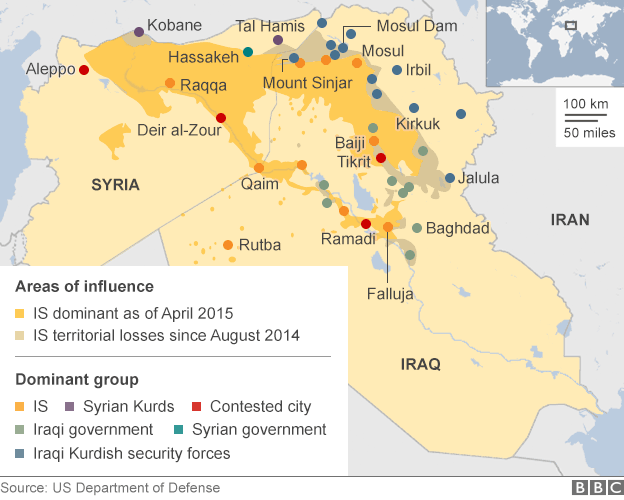
\includegraphics[trim = 0cm 0cm 0cm 0cm, clip,scale=0.5]{./figures/current_territory.png}
   \caption{Current ISIL Territory \cite{BBC2015a,Lewis2014}}
     \label{fig:current_territory}
\end{figure}



% \begin{figure}[H]
%  \centering
%  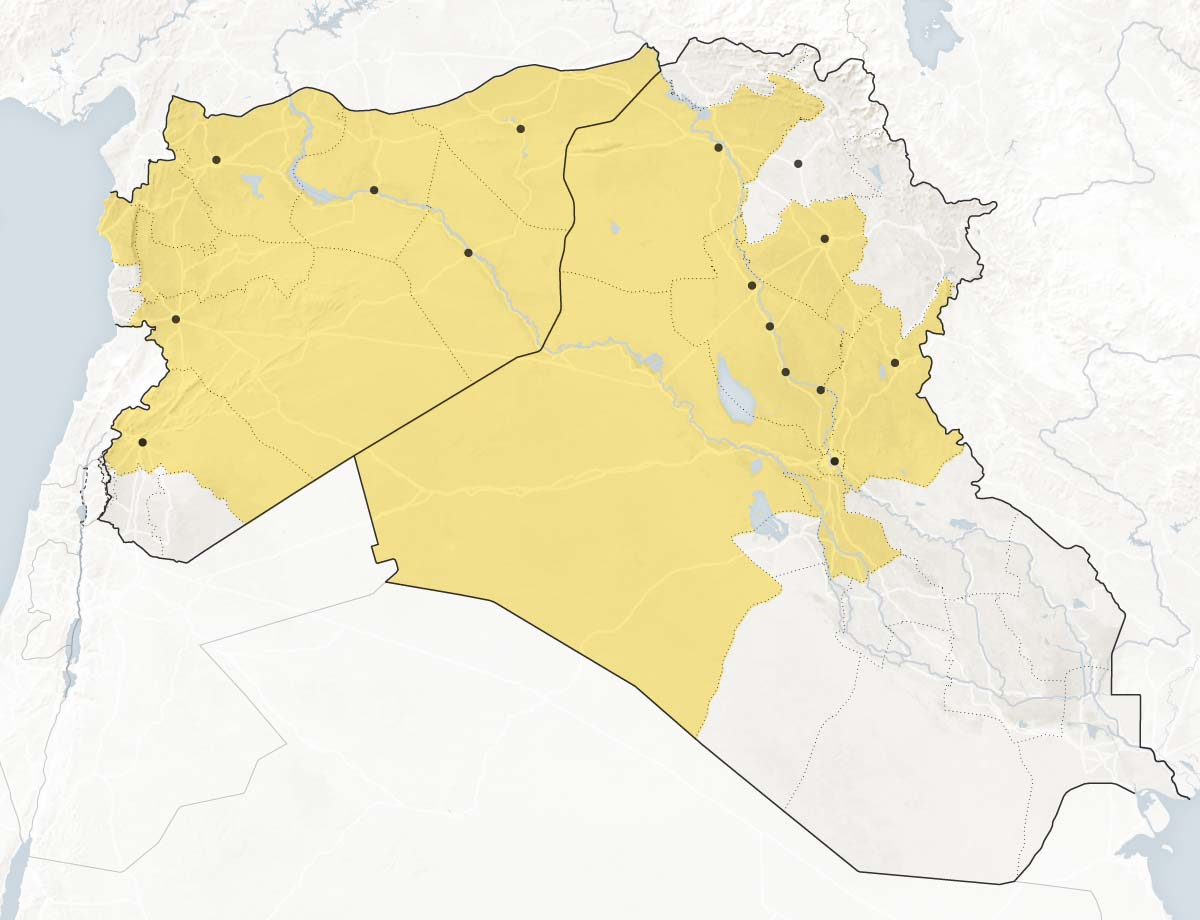
\includegraphics[trim = 0cm 0cm 0cm 0cm, clip,scale=0.3]{./figures/current2.png}
%    \caption{What ISIL Wants \cite{Lewis2014}}
%      \label{fig:current2}
% \end{figure}



\begin{figure}[H]
 \centering
 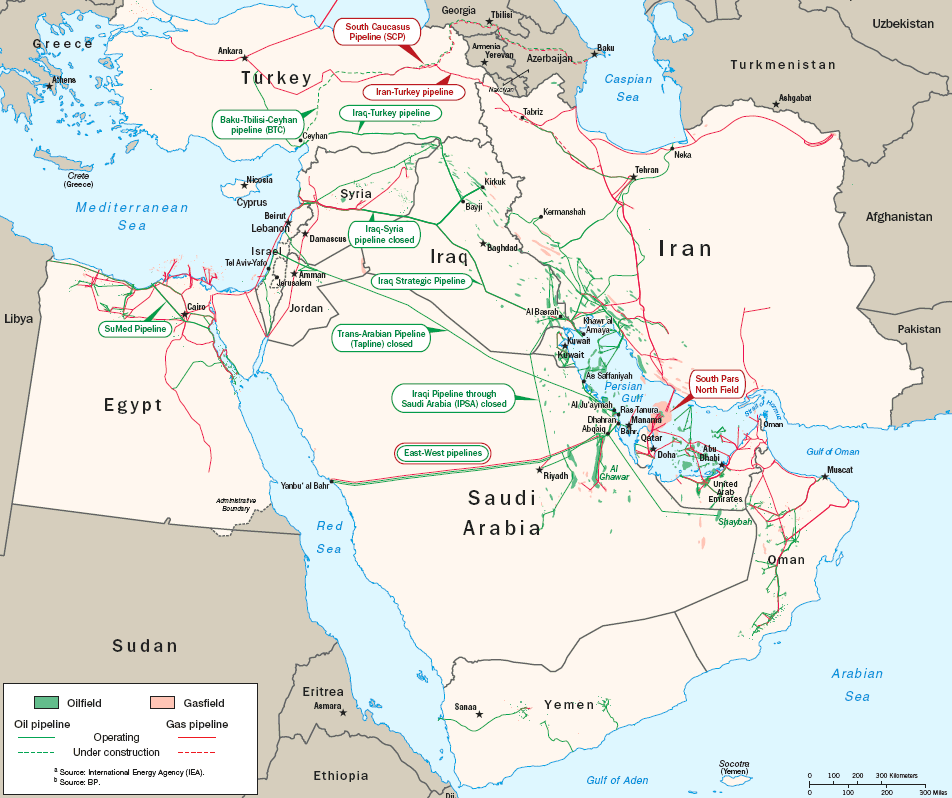
\includegraphics[trim = 0cm 0cm 0cm 0cm, clip,scale=0.3]{./figures/oil_reserves.png}
   \caption{Oil Reserves and Ground Transportation Routes \cite{PoliticalCalculations2012}}
     \label{fig:oil_reserves}
\end{figure}



\begin{figure}[H]
 \centering
 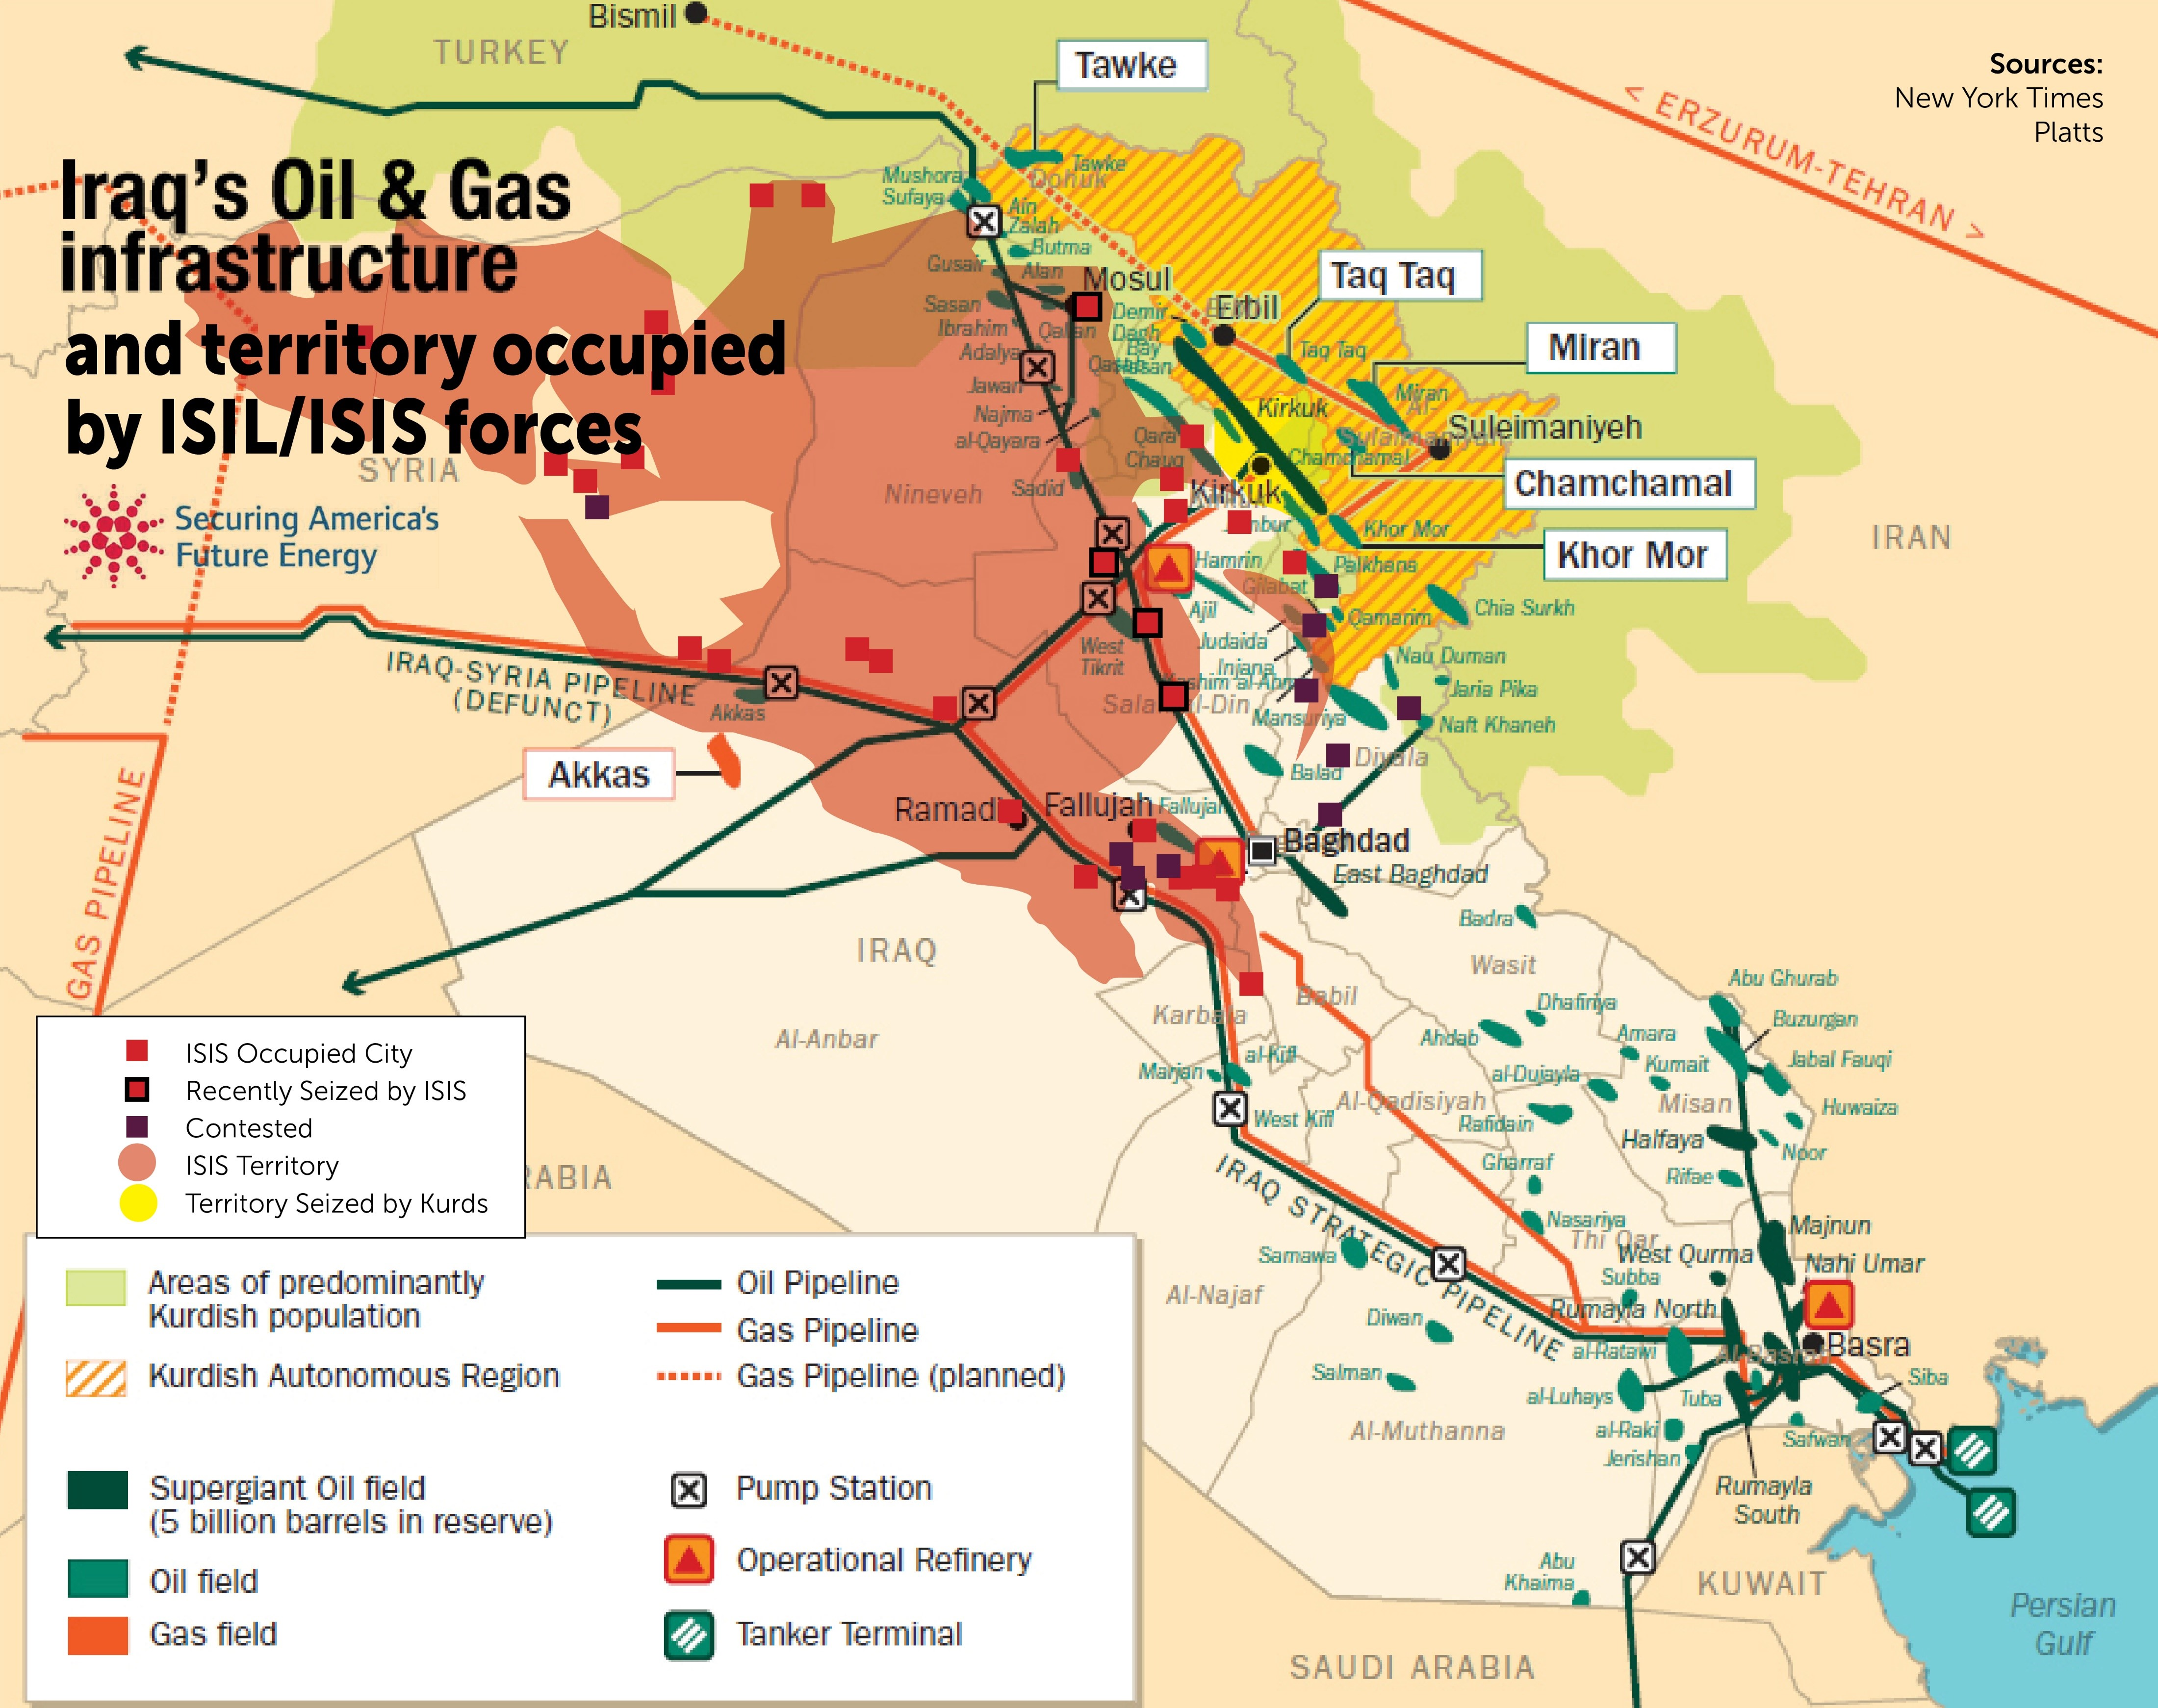
\includegraphics[trim = 0cm 0cm 0cm 0cm, clip,scale=0.3]{./figures/oil_infrastructure.jpg}
   \caption{Iraq's Oil \& Gas Infrastructure \cite{EnergyPolicyInformationCenter2014}}
     \label{fig:oil_infrastructure}
\end{figure}



\begin{figure}[H]
 \centering
 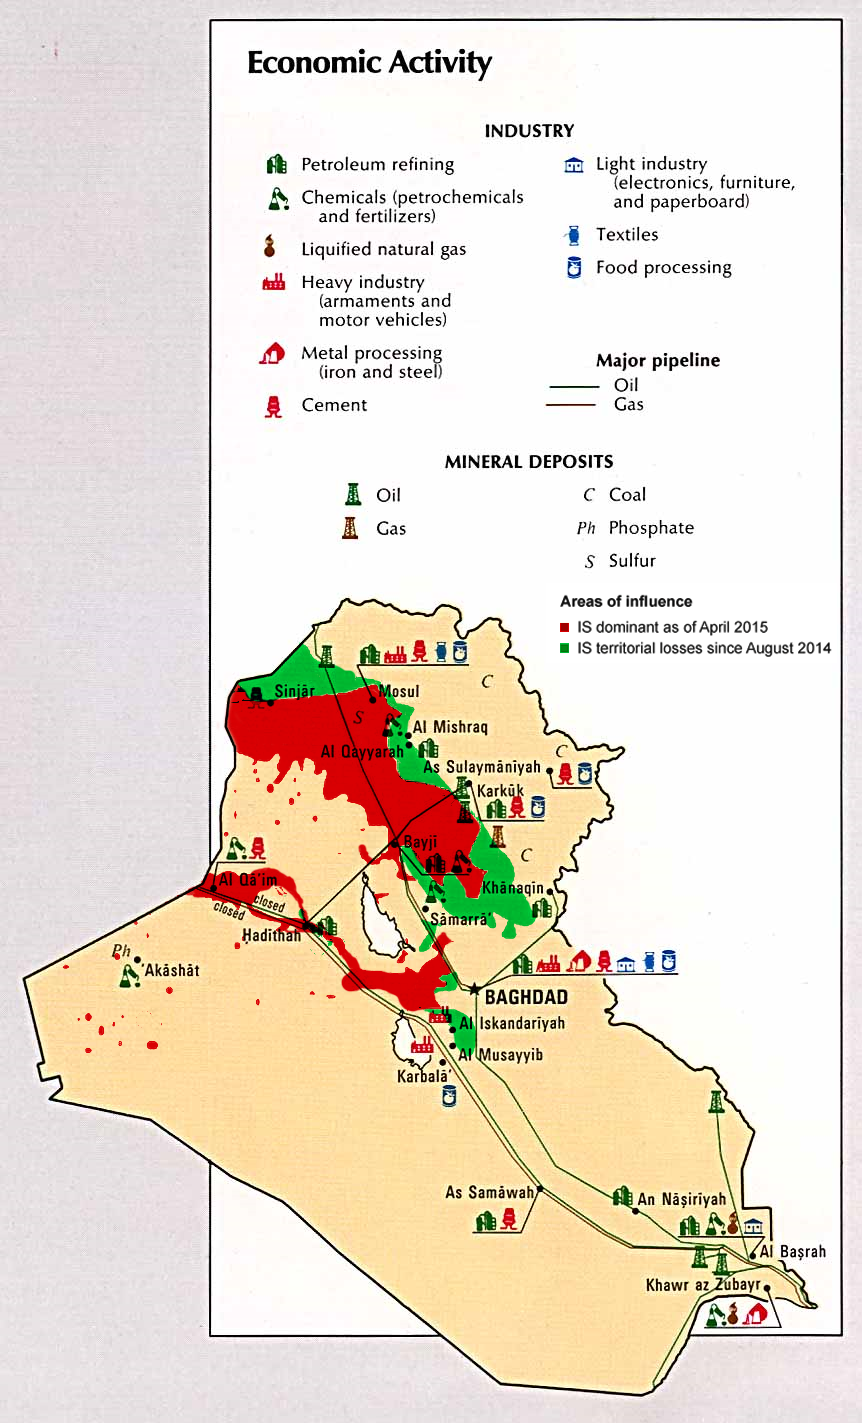
\includegraphics[trim = 0cm 0cm 0cm 0cm, clip,scale=.3]{./figures/minerals2.png}
   \caption{Mineral Deposits and Industry in Iraq, with current ISIL territory overlay \cite{Ellis2005}}
     \label{fig:minerals}
\end{figure}




\begin{figure}[H]
 \centering
 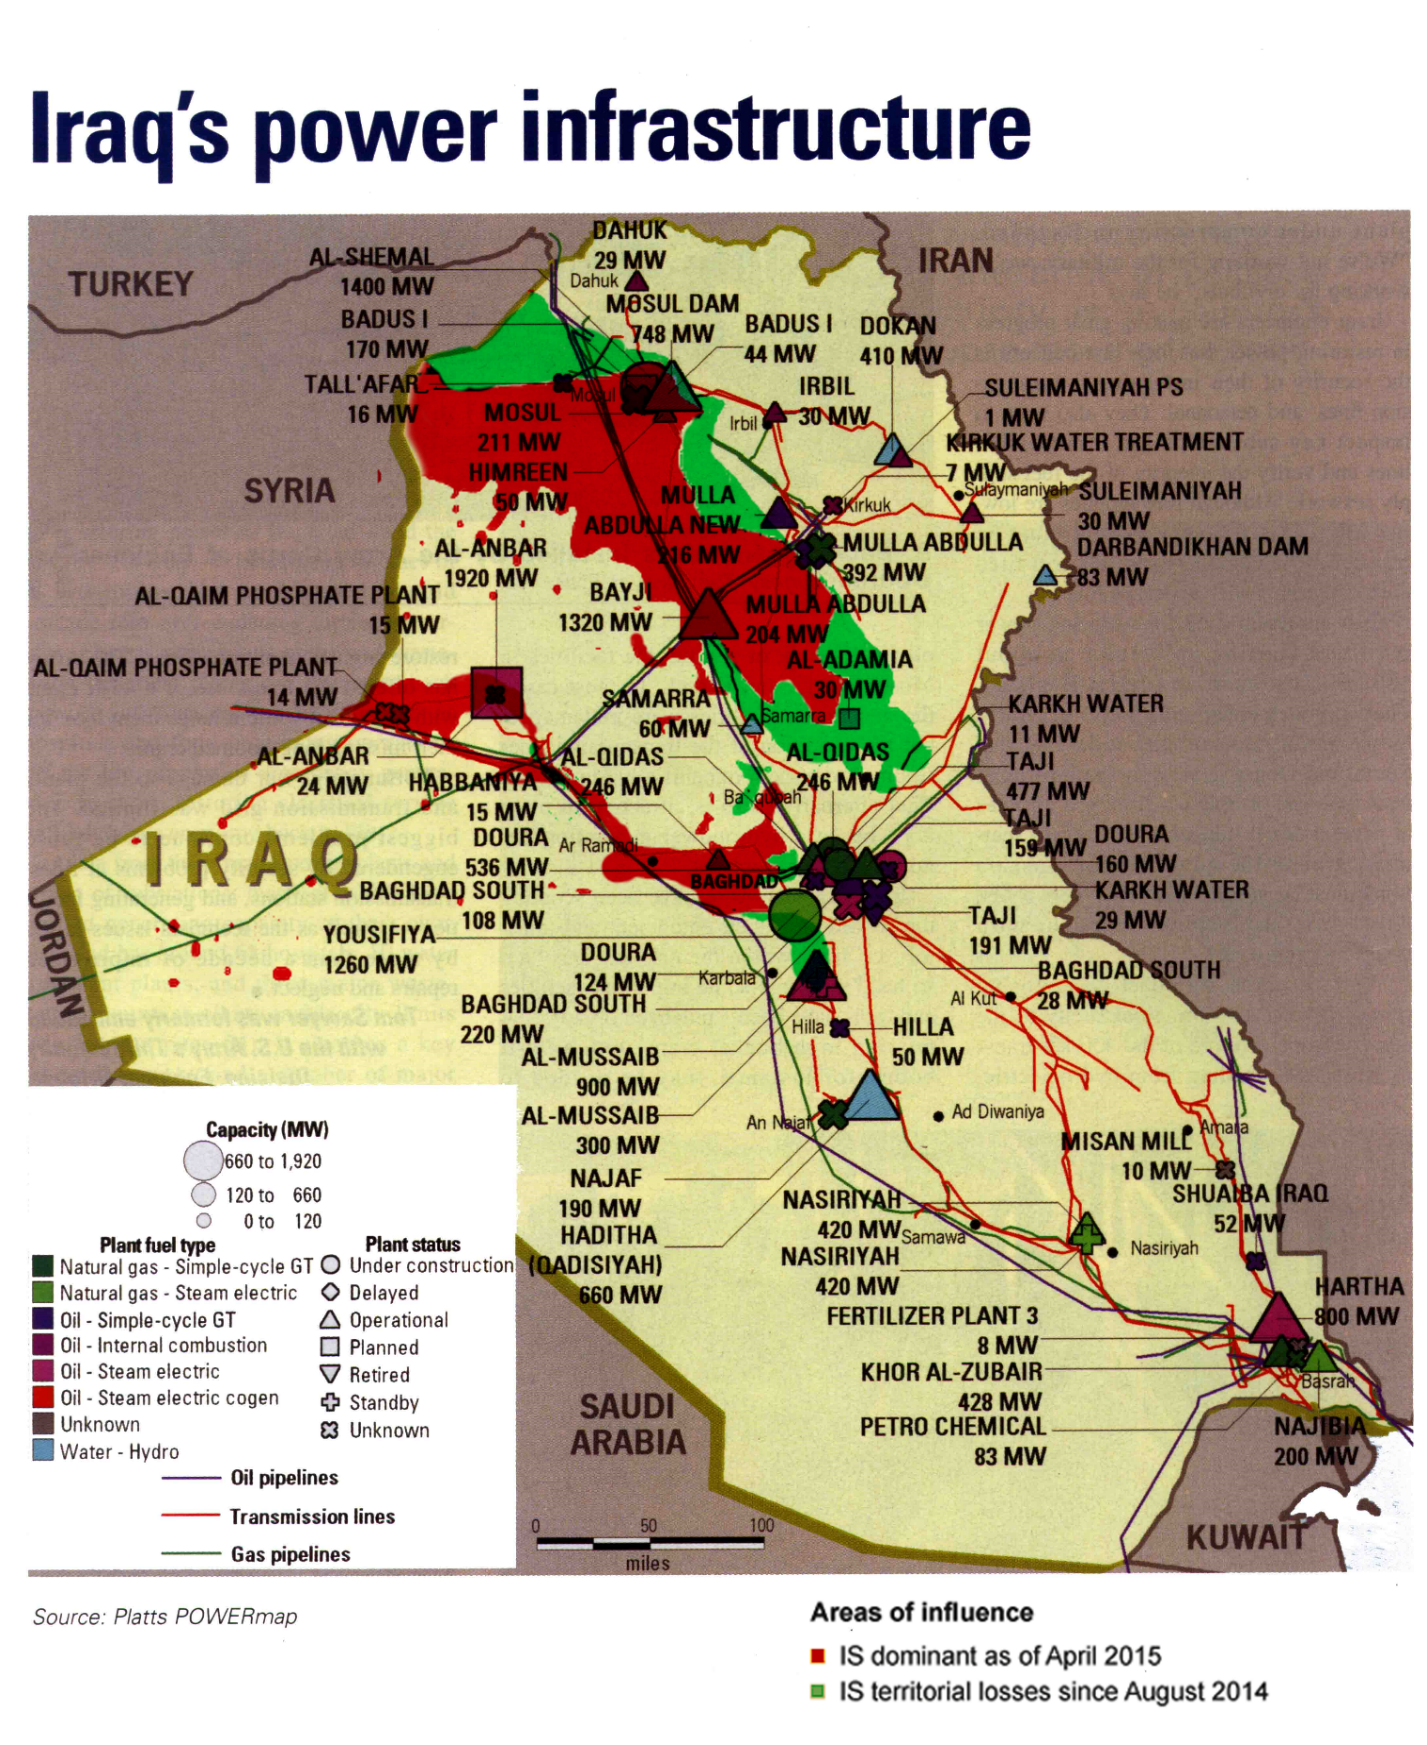
\includegraphics[trim = 0cm 0cm 0cm 0cm, clip,scale=.3]{./figures/elec_grid2.png}
   \caption{Iraqi Electricity Grid, with current ISIL territory overlay \cite{GlobalEnergyNetworkInstitute}}
     \label{fig:elec_grid}
\end{figure}







\begin{figure}[H]
 \centering
 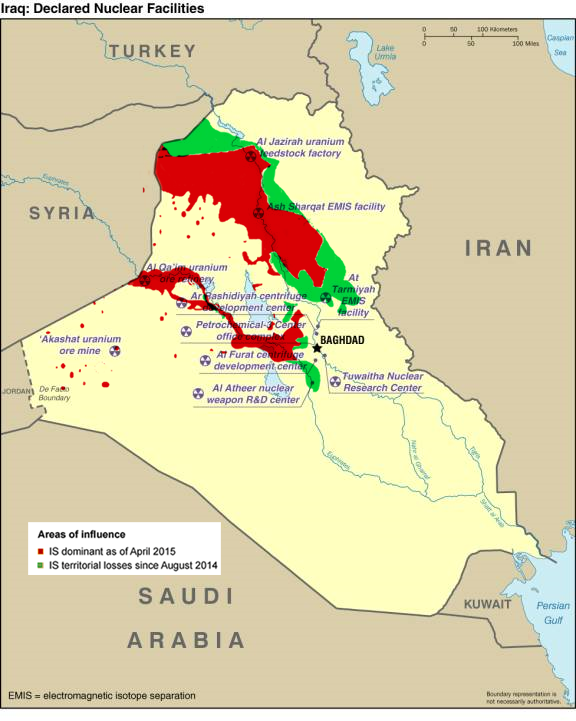
\includegraphics[trim = 0cm 0cm 0cm 0cm, clip,scale=.6]{./figures/nuke_facilities2.png}
   \caption{Iraq Declared Nuclear Facilities (as of 2002), with current ISIL territory overlay \cite{Fox2002}}
     \label{fig:nuke_facilities}
\end{figure}









\begin{figure}[H]
 \centering
 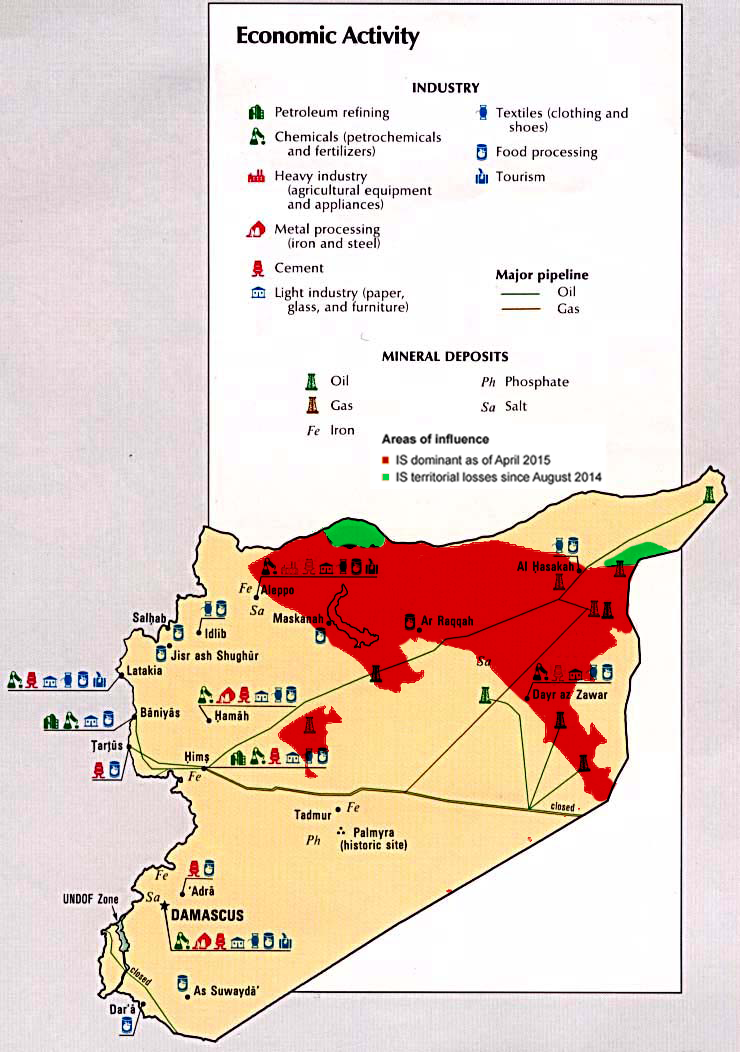
\includegraphics[trim = 0cm 0cm 0cm 0cm, clip,scale=0.5]{./figures/syria_minerals2.png}
   \caption{Mineral Deposits and Industry in Syria,  with current ISIL territory overlay \cite{Ellis2005}}
     \label{fig:syria_minerals}
\end{figure}





\begin{figure}[H]
 \centering
 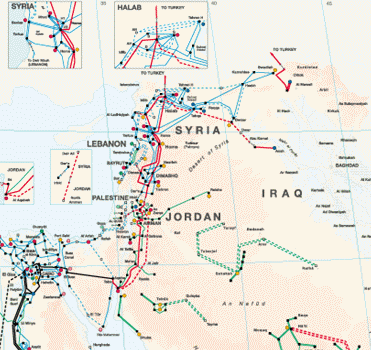
\includegraphics[trim = 0cm 0cm 0cm 0cm, clip,scale=1]{./figures/syria_grid.png}
   \caption{Syrian Electricity Grid \cite{GlobalEnergyNetworkInstitutea}}
     \label{fig:syria_grid}
\end{figure}






\begin{figure}[H]
 \centering
 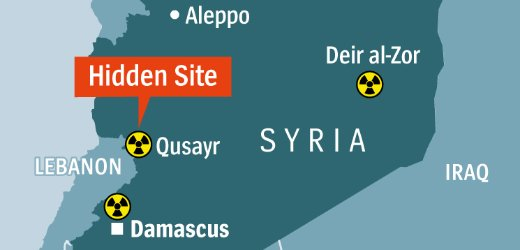
\includegraphics[trim = 0cm 0cm 0cm 0cm, clip,scale=0.7]{./figures/syria_nuke_facilities.jpg}
   \caption{Syrian sites of possible nuclear facilities \cite{Follath2015}}
     \label{fig:syria_nuke_facilities}
\end{figure}










\section{RDD: Radioactive Sources}

\subsection{???? STILL MISSING?????}

STILL MISSING!!!

Placeholder for Eric Harvey's missing section on orphan / medical sources policy.


% \subsubsection{RDD}
%  Some of the materials required to build an RDD are naturally occurring elements that are naturally radioactive. Other components are solely available to radiological work sites such as reactor facilities, isotope production, research and universities, weapons production facilities, and other commercial and industrial facilities. 
% 
% The lands surrounding ISIL are vast, and currently a large majority are under militant occupation.  The probability that materials of this nature can move about the region is very high.  Paid courier services, as well as stolen armed and armored transportation vehicles  may assist in this endeavor.
% 
% \subsubsection{???????? Identify possible and likely sources of the top 10 RDD materials identified in section 2.2 that ISIL might purchase or steal. Also identify possible sources of these materials within territory that ISIL controls (such as hospitals and universities). Discuss any current export controls on these materials, and how they might inhibit the acquisition of significant quantities of materials. Discuss the orphan source program, or any other international institutions which regulate the creation and distribution of radioactive sources. (To be added by 4/19; possible add map of sources?) ?????????????} 








\section{Illicit Trafficking} \label{sec:Trafficking}


\bfseries Targeted Capability: SNM/Complete Warhead 

Pathway: Illicit Trafficking 

Existing Policy: \textcolor{red}{Second Line of Defense Core Program} 

Proposed Policy: \textcolor{red}{Increase SLD locations in Syria}

Lead Agency: NNSA

Contributing Agency: DNDO, DTRA, DoS, Bechtel Nevada  \normalfont



In the event that ISIL attempts to acquire SNM, the core of a nuclear weapon, or a complete weapon, it is likely that it will need to be smuggled internationally. It is in the U.S.'s best interest to prevent a nuclear weapon or SNM from entering the controlled territory of ISIL. There are two methods of trafficking SNM or a complete weapon, overland and overseas. Trafficking of a complete weapon over land would be difficult due to the heavy weight of the weapon. However, the SNM is relatively light weight and volume-wise very small, and it is very likely that over land routes would be used. ISIL is extremely proficient at smuggling and makes millions of dollars a day from smuggling everything from oil to humans \cite{Amos2014}. Due to this massive illicit trafficking infrastructure already set up, it is unlikely that any effort to intercept these SNM overland would likely succeed. However, prevention of smuggling SNM overseas through the ports is much more feasible. 

To prevent the smuggling of nuclear materials, the U.S., NNSA started the Second Line of Defense (SLD) Core Program  \cite{Kilmartin2010}. This program installs radiation detection equipment at borders, airports, and strategic feeder ports in Russia, former Soviet Union states, and other key countries \cite{Kilmartin2010}. While not specific to the ISIL crisis, it does help hinder any attempts for ISIL to smuggle nuclear materials/weapons. To adapt the SLD for use against ISIL, it is proposed to add SLD port monitors at the Port of Lattakia and the Port of Tartous (see \autoref{fig:seaports}), which are the closest ports to ISIL-controlled territory that have container liner services \cite{WorldPortSource2005}.  By adding two more ports to this list, the likelihood of ISIL succeeding in smuggling a nuclear weapon/materials can be dramatically reduced. In general it is estimated to cost \$3.75 million dollars per port and would take one year to implement \cite{Aloise2005}. 

The NNSA is the lead agency and would be responsible for developing the strategic direction of the implementation as well as providing project performance and financial oversight. The main contributors would be the Domestic Nuclear Detection Office (DNDO), Pacific Northwest National Laboratory (PNNL), and Bechtel Nevada. The facilities at the DNDO will be used for testing purposes with the support of Bechtel Nevada. PNNL will be the lead organization for providing training to countries participating in the SLD. Bechtel Nevada will be responsible for routine and preventative maintenance for the equipment deployed overseas \cite{NationalNuclearSecurityAdministration2006}. 





\begin{figure}
 \centering
 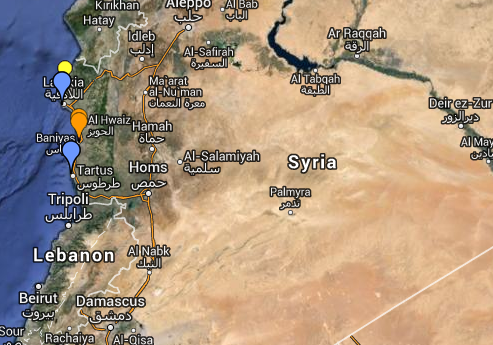
\includegraphics[trim = 0cm 0cm 0cm 0cm, clip,scale=0.85]{./figures/seaports.png}
   \caption[Location of the five seaports in Syria \cite{WorldPortSource2014}.]{Location of the five seaports in Syria. Of these only the blue-colored ones (Port of Lattakia and the Port of Tartous) have container liner services \cite{WorldPortSource2014}.}
     \label{fig:seaports}
\end{figure}





\section{Theft}


\subsection{IAEA Monitoring}



\bfseries Targeted Capability: SNM/Complete Warhead

Pathway: Theft

Existing Policy:  \textcolor{red}{IAEA Monitoring \& the Additional Protocol}

Proposed Policy:  \textcolor{red}{Push for AP signatures from high risk countries (Egypt, Syria, \& Pakistan)}

Lead Agency: DoS, ISN

Contributing Agency: DTRA \normalfont

The targeted capability of concern for this policy is the theft or diversion of SNM for a nuclear weapon or the theft or diversion of a complete warhead. The pathway intended for intercept is through theft or purchase, and the interception method is IAEA monitoring under the NPT Comprehensive Safeguards Agreements and, where possible, the Additional Protocol (AP). The proposal to strengthen this interception method is to negotiate with states at risk of supporting ISIL willingly or unwillingly to accept NPT AP measures to strengthen safeguards on their SNM and, if existing, any nuclear weapons the state possesses. This will help to break the links connecting \enquote{Steal} and \enquote{Purchase} on the logic tree in \autoref{fig:logic_tree} with any material needed for nuclear weapon acquisition that is covered in the NPT safeguards, including \enquote{Thermonuclear Device}, \enquote{Fission Device}, \enquote{RDD}, and \enquote{SNM}. 



The purchasing of nuclear materials, while it could be done on a national level, is much more likely to occur through individuals. The only collection of nation confirmed information on incidents of illicit trafficking and other unauthorized activities involving nuclear and other radioactive material is called the Incident and Trafficking Database (ITDB) and is maintained by the IAEA. As of 2006, over 1000 incidents of illicit trafficking and other unauthorized activities involving nuclear and other radioactive material has been reported to the IAEA with about 25\% specifically involving nuclear materials \cite{Iaea2007}. A majority of these cases involve highly enriched uranium (no plutonium). One such incident occurred in 1994 when an individual stole 2.972 kg of highly enriched uranium from a nuclear factory \cite{Iaea2007}. See \autoref{fig:seizures} for more information on the location and size of notable seizures. 

\begin{figure}
 \centering
 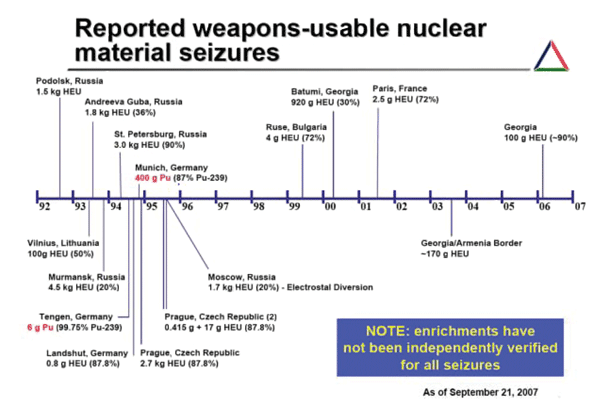
\includegraphics[trim = 0cm 0cm 0cm 0cm, clip,scale=0.7]{./figures/seizures.png}
   \caption{Location and time of global seizures of special nuclear materials \cite{Muller2007}.}
     \label{fig:seizures}
\end{figure}


Most of these instances are very small amounts (grams) but there have been several involving one to three kilograms. No individual case has been found with enough material to make a nuclear bomb, but multiple thefts could allow ISIL to accumulate enough special nuclear material to create a nuclear weapon. 


The lead U.S. agency responsible for implementing this policy will be the U.S. Department of State  supported by the U.S. Defense Threat Reduction Agency. Preventing ISIL from acquiring a nuclear weapon, or at the very least SNM, falls under the purview of both the Bureau of Counterterrorism and the Bureau of International Security and Nonproliferation (ISN) within the DoS. Under this policy strategy, ISN is the principal actor in the DoS as they are the primary U.S. interface with the IAEA on the NPT \cite{Circular1970}. DTRA is a Combat Support Agency that supports the Combatant Commanders and Services in responding to any WMD threat. One aspect of this support is managing a research and development portfolio to develop tools and capabilities to detect and respond to WMD threats. DTRA is the agency within the U.S. government that works to verify treaties related to WMD are being carried out by all signatories, and thus will be able to support the DoS ISN in this policy \cite{DefenseThreatReductionAgency}. 

The AP is \enquote{a legal document granting the IAEA complementary inspection authority to that provided in underlying safeguards agreements} \cite{InternationalAtomicEnergyAgency1997}. The AP's purpose is to enable the IAEA inspectorate to provide assurances on declared and possible undeclared activities in order to have a more complete picture of a state's overall nuclear program. The IAEA is granted increased access to information and sites under the AP. Of the 188 UN member states whom are party to the NPT, there are a total of 124 APs (plus Taiwan and Greenland) in force. Considering again \autoref{fig:affmap}, the states of primary concern that are either not already party to the NPT or have not ratified the Additional Protocol include Algeria, Egypt, Sudan, South Sudan, Saudi Arabia, Yemen, Syria, and Pakistan \cite{DefenseThreatReductionAgency,InventoryofInternationalNonproliferationOrganizationsandRegimes2013}. Of these states, the ones with significant nuclear capabilities that are of most concern are Egypt, Syria, and Pakistan, with Pakistan being of the most concern as they are not party to the NPT and have substantial nuclear capabilities, including an existing nuclear weapon stockpile \cite{InventoryofInternationalNonproliferationOrganizationsandRegimes2013}. North Korea is a wild card for this policy, but is unavailable through NPT and AP negotiation channels as they are not party to the NPT nor are they considered open to U.S. negotiation in general. 

Therefore, this proposed policy is to negotiate with states in proximity and with ties to ISIL, particularly Egypt, Syria, and most importantly Pakistan, to accept additional IAEA NPT safeguards under the AP. Pakistan is an interesting challenge as they are not party to the NPT, but there is precedence in the case of India for strengthening IAEA NPT Safeguards through customized AP agreements. The budget for this policy is inherently small, and the schedule is longer term due to the slower mechanisms of politics.  However, it is important to pursue this policy now in order to convince the states of concern that the U.S. is open to negotiation and will not tolerate willing or unwilling support of ISIL. With a limited budget, the tools for negotiation will be so-called \enquote{carrots} and \enquote{sticks}. Carrots may include increased cooperation and development of peaceful applications of nuclear technology under the NPT regime, or increased economic trade and development with the cooperating state if nuclear energy is not a priority. Sticks may include economic sanctions, and, in more extreme cases, UN-wide sanctions.



\subsection{UNSCR-1540 Nuclear Security Standards}



\bfseries Targeted Capability: SNM/Complete Warhead

Pathway: Theft

Existing Policy:  \textcolor{red}{UNSCR-1540 Nuclear Security Standards}

Proposed Policy:  \textcolor{red}{Export nuclear security training}

Lead Agency: DoT, DoD

Contributing Agency: NNSA  \normalfont


The proliferation of  WMD is a serious national and international security threat. A possible pathway of ISIL obtaining SNM and complete warheads is theft.  UNSCR-1540 is directed at maintaining peace by preventing the proliferation of  WMD. This resolution proposes key actions aimed at non-proliferation \cite{Gomes2007a}:


\begin{easylist}[enumerate]
& Withholding any supportive actions of non-UN-member States having chemical, biological and nuclear weapons.
& UN members should have appropriate laws that prevent  non-member States from development, manufacturing, obtaining, transportation, and usage of nuclear weapons.
& States should have an appropriate system of internal control for non-proliferation of chemical, biological, and nuclear weapons, including control over the crucial materials for the WMD. In order to achieve these goals, States should develop:
&& A system to effectively account for items and materials related to  chemical, biological, and nuclear weapon processing, usage, transportation, and storage.
&& A system of physical protection for items and materials related to chemical, biological, and nuclear processing, usage, transportation, and storage.
&& A control system to detect, stop, and combat (within international law if needed) the illegal transportation of  items and/or materials for chemical, biological, and nuclear weapons.
& Creation of a Committee of the Security Council that will inspect the execution of the current resolution and will report the results to the Security Council.
& Recommends all UN member States to:
&& Put more effort on improvement of multilateral treaties about prevention of  chemical, biological, and nuclear weapons.
&& Accept national regulations for prevention of proliferation, which will have compliance with the multilateral  and international non-proliferation treaties.
& Recommends the States to be more active in nonproliferation cooperation aimed to prevent illegal trafficking of chemical, biological, and nuclear weapons, related items and materials, and their methods of delivery.
& Recognizes that some States might want to request  assistance for execution of the above resolutions. Assistance might be in terms of skills and resources that are  crucial to achieve the provisions above.
\end{easylist}


% Proposed Policy: Export Nuclear Security Training

Implementation of these rules would limit the proliferation of WMDs. However, there might be States with nuclear weapons where nuclear facilities have low physical security levels. These facilities are vulnerable to the theft of nuclear weapons and/or materials by ISIL, an organization that has the military and financial capability to successfully complete such an operation.

Global Security estimates the total assets of ISIL at \$500 billion \cite{GlobalSecurity}. Their  military capacity is estimated to include about 31,000 fighters \cite{BBC2014}. To prevent risk of proliferation, actions toward security improvements should be taken. First of all, highly vulnerable nuclear facilities that contain nuclear warheads, materials, and technology should be given the same defense as in Provision \#7 of the UNSCR-1540 \cite{Gomes2007a}. 

Furthermore, the Committee of the Security Council should be given greater enforcement power to bring together the international community in order to respond quickly to the threat of ISIL. It should also engage in training  to equip nuclear states with low security and highly vulnerable nuclear facilities. Security training would include personnel training and the use of surveillance and other technologies to prevent  unauthorized access. 

A barrier to assessing the necessary level of security training  is that IAEA does not know the condition of those facilities in countries that have not signed the NPT. Pakistan, India, and Israel do not allow IAEA inspectors to investigate or visit their nuclear facilities, thus the security training cannot be catered to the specific country.  Therefore, nuclear training can occur in two ways:


\begin{easylist}[enumerate]
& International Atomic Energy Agency (IAEA) runs over 60 nuclear security and education training events each year \cite{InternationalAtomicEnergyAgency2014}. These events cover the different aspects of nuclear facility security, including physical protection, identification of weak points of nuclear facility security, and information security.
& Exporting security training to the nuclear facilities of the countries that request assistance, according to Provision \#7 under the USCR-1540 \cite{Gomes2007a}. This will allow for more accuracy in giving proper training to the countries, by tailoring it to the special features of the locations.
\end{easylist}


We suggest that the United Nations  extend UNSCR-1540 to adding provisions about nuclear security training. We must also provide incentives to UN members and non-UN-member countries to attend the nuclear security educational events hosted by IAEA. Moreover, training needs to heavily focus on managing and securing  chemical, biological, and/or nuclear weapons materials and facilities. 

% Budget and Implementation Time 

The IAEA's Education and Training in Nuclear Security is a subgroup of IAEA's Nuclear Safety and Security. The budget of  Nuclear Safety and Security is about 37 million Euros  as of 2015 \cite{Iaea2014}. Since these trainings are held annually by the IAEA, there is no need for additional financing for visitor countries. However, for export training, additional financing is required. Even so, financing should not exceed more than a few hundred thousand dollars per year, per training. 

The time for the implementation of an  expert group specializing in nuclear training can range from six months to a year, based on past experience.  Training groups can be built from the same groups in the IAEA that hold nuclear security and education events. The U.S Department of Transportation and NNSA  will work in conjunction with countries to help them implement safety across borders to prevent the movement (theft) of nuclear material. 




\subsection{Global Threat Reduction Initiative} \label{sec:GTRI}



\bfseries Targeted Capability: SNM/Complete Warhead

Pathway: Theft

Existing Policy:  \textcolor{red}{Global Threat Reduction Initiative}

Proposed Policy:  \textcolor{red}{Renew and broaden GTRI commitment; emphasize international  collaboration }

Lead Agency: NNSA


Contributing Agency: DTRA, DoD, NNSA, NPWG  \normalfont



% GTRI existing policy :

The Global Threat Reduction Initiative (GTRI) prevents nuclear material from getting into the wrong hands by removing SNM from improperly protected facilities, converting nuclear  reactors from highly enriched uranium (HEU) to low enriched uranium (LEU), and improving security at nuclear facilities that are vulnerable to theft or sabotage \cite{NationalNuclearSecurityAdministration2014}. Thus far, 49 HEU research reactors have been converted or shut down. Currently, security enhancement involves installation of detectors, such as Passive Infrared Sensors (PIR), Remote Monitoring Systems (RMS), and Personal Radiation Detectors (PRD) \cite{NationalNuclearSecurityAdministrationa}. Courses have been developed to train personnel of nuclear facilities on how to use the advanced detectors and equipment to secure their nuclear facilities, as well as how to respond in case of potential theft or sabotage. GTRI should provide travel funding for people to attend courses where they can get a theoretical basis and hands-on security experience. GTRI is also collaborating with universities to create a nuclear security curriculum.

% Proposed policy

The GTRI should continue to provide assistance to domestic nuclear facilities to remove unused nuclear material, enhance security in storage and transport of nuclear material, and increase training to local law enforcement. 

The GTRI should put emphasis on establishing collaboration with international organizations and countries throughout the world to enhance nuclear security.  In addition to working directly in foreign countries, GTRI should provide training and equipment to local state agencies, to enable them to assure the safety of their nuclear facilities. 

Russia still houses the largest quantities of radioactive material and has dozens of nuclear reactors that still use HEU fuel.  Bilateral agreement with countries such as Russia should be established in addition to the GTRI to allow close adjustment to the specific situation. 

% Budget and Implementation 

Converting or possibly shutting down the 200 HEU research reactors is expected to be completed by 2035, under the current budget plan.  By 2018, 98\% of excess and vulnerable weapons-grade material will be removed \cite{Position2014}. 8,500 buildings   with high-priority nuclear and radiological material will be secured, predicted to be finished in 2044 \cite{Roth2014}. The budget for fiscal years 2012, 2013, and 2014 are \$503,453, \$501,048 and \$424,487, respectively. 






\subsection{Bilateral Nuclear Security Agreements}



\bfseries Targeted Capability: SNM/Complete Warhead

Pathway: Theft

Existing Policy:  \textcolor{red}{Bilateral Nuclear Security Agreements}

Proposed Policy:  \textcolor{red}{Strengthen existing bilateral arrangements; Engage Iran and North Korea}

Lead Agency: DoS


Contributing Agency: DoD, DoE  \normalfont



\textbf{Russia}

The U.S. signed the New Strategic Arms Reduction Treaty (New START) with Russia on 8 April 2010, and the treaty entered into force on 5 February 2011. The treaty limits the number of deployed strategic nuclear weapons to 1,550 on each side, to be achieved by February 2018. Deployed ICBMs, SLBMs, and heavy bombers assigned to nuclear missions are limited to 700, and deployed and non-deployed ICBM launchers, SLBM launchers, and bombers are limited to 800. Non-deployed ICBMs and SLBMs will also be monitored through on-site inspections and must be located at specified facilities away from deployment sites, labeled with unique identifiers \cite{U.S.DepartmentofState2015}. 

New START provides a verification mechanism that allows both sides to keep check on each other's nuclear capabilities, building transparency and confidence. Importantly, the treaty will also keep account of all SNM/warheads that exist, not only for the benefit of U.S.-Russia nuclear relations but also for the possibility of nuclear weapons proliferation at the hands of non-state actors like ISIL.

\textbf{Policy recommendations:}

The U.S. should maintain New START as one of the options to strengthen the overall verification process of nuclear weapons, missiles and launchers, as a means to ensure global nuclear weapons security. New START has been under the purview of the U.S. Department of State, working in conjunction with the U.S. Department of Defense.

Up to 2012,  the cost of implementation of  New START has been U.S. \$301 million \cite{U.S.DepartmentofDefense2012}. Although  New START is not put into effect with the aim of preventing ISIL, it will have have positive complementary effects. Presumably, it will make it more difficult for ISIL to obtain and transport nuclear weapons and material through theft because of increased nuclear security. 



\textbf{Pakistan}

One of the most troublesome aspects of Pakistan's highly vulnerable nuclear  facilities is the high likelihood of theft by ISIL. Although the U.S. has been very supportive of Pakistan's efforts to ensure its nuclear weapons security, there are various challenges that could still undermine Pakistan's efforts. Pakistan has received various military and non-military aid, close to U.S. \$28.4 billion  since 9/11 \cite{Upadhyay2014}. 

\textbf{Policy recommendations:}

The U.S. needs to continue to assist Pakistan in increasing its nuclear security capabilities, by providing monetary assistance and military hardware, as well as services such as training and intelligence sharing. The U.S. Department of State has been the lead agency in maintaining the U.S.-Pakistan bilateral relations; however, when military-specific assistance is needed, DoS will work closely with the U.S. Department of Defense on this issue.


\textbf{North Korea}

North Korea's nuclear capabilities and hostile leadership are distressing elements with respect to the growing threat of ISIL and global efforts to achieve nuclear weapons security. Because of that, North Korea's lack of cooperation poses one of the largest threats to ensuring that ISIL does not acquire, transport, or trade nuclear weapons.

The absence of diplomatic relations with North Korea stems from North Korea's attempted annexation of South Korea, resulting in the Korean War and U.S. imposed economic sanctions on North Korea \cite{U.S.DepartmentofState2015a}. The only communication between the two countries has been under the Six-Party Talks for the Denuclearization of the Korean Peninsula. Most forms of U.S. economic assistance, other than purely humanitarian assistance, are prohibited; therefore, U.S. assistance has been limited to food or energy aid. Between 1995 and 2001, the U.S. has spent more than U.S. \$1.3 billion  in total aid to North Korea (food aid - U.S. \$708 million, energy assistance - U.S. \$404 million, Six-Party Talks-related assistance - U.S. \$191 million) \cite{Manyin2014}.

\textbf{Policy recommendations:}


The U.S. should continue the Six-Party Talks and begin actively engaging North Korea. Historical memory and isolation from the international world has made North Korea extremely hostile to the U.S. However, North Korea desires international legitimacy and has claimed that it wants to be a responsible nuclear power. Building upon that objective, North Korea and the U.S. can form multilateral agreements with China and South Korea aimed at preventing theft or sale of weapons through securing nuclear weapons facilities. Eventually, conditional agreements could be put in place where North Korea allows IAEA inspectors, in exchange for food or energy. 


\textbf{Iran}

The U.S. also need to address Iran's nuclear ambitions.  The U.S. is working under P5+1 initiatives to negotiate a nuclear deal to halt Iran's nuclear development. This cooperation will ensure monitoring and verification of Iran's nuclear development. Although it is known that Iran and ISIL have opposing ambitions and will likely not cooperate together, Iran's nuclear capabilities could also lead to proliferation of nuclear weapons into non-state actors and future proxy wars involving nuclear weapons \cite{Pfarrer2014}.

\textbf{Policy recommendations:}

The U.S. should work with Iran to prevent ISIL's acquisition of nuclear weapons. Easing economic sanctions and welcoming Iran into the international community will help facilitate bilateral relations for the mutual goal of defeating ISIL.  
 

 







\section{Gift/Purchase} \label{sec:purchase_gift}



\bfseries Targeted Capability: SNM/Complete Warhead

Pathway: Gift/Purchase

Existing Policy: \textcolor{red}{Nuclear Forensics Attribution Act}

Proposed Policy: \textcolor{red}{Declaratory policy on use of force for nuclear technology transfer}

Lead Agency: DoS, DNDO/NTNFC

Contributing Agency: DoD, IC, NNSA, DTRA \normalfont

The targeted capability of concern for this policy is the ability of ISIL to obtain a complete nuclear weapon or components of a nuclear weapon via purchase or gift from a nuclear capable state.  Given our general lack of insight into foreign nations' nuclear weapons programs, locations, security, and accountability measures (at least in the open literature), it is impossible to develop a policy aimed at preventing the sale or gift of nuclear weapons or nuclear weapons components at the source.  Instead, the policy recommendation focuses on strengthening existing nuclear forensics capabilities to positively attribute any nuclear detonation to the country of origin while simultaneously issuing a declaratory policy on the U.S. response of the use of nuclear weapons against the U.S. or its allies.  Specifically, this declaratory policy would focus on the U.S. response to the transfer of nuclear technology, materials, or weapons that result in a detonation of a nuclear weapon on the U.S. or one of its allies.  This policy would close any potential loopholes in the Nuclear Posture Review's (NPR) declaratory policy and provide a tangible disincentive for the illicit proliferation of nuclear technology, materials, or weapons to ISIL \cite{U.S.DepartmentofDefense2010}.  

Key to this policy option is the ability to definitely identify weapon characteristics including the country of origin, date of manufacture, and weapon design.  As discussed in \autoref{sec:post_det_forensics}, the U.S. and international capability maintains the ability to provide both pre- and post-detonation forensics of nuclear materials and weapon components that can be used in the attribution process.  The Nuclear Forensics and Attribution Act (NFAA) of 2010 provides guidance for the development and processing of nuclear forensics information, but it stops short of stating the end use of such information \cite{Act2010}.  The NFAA established the NTNFC within the DNDO \enquote{to provide centralized stewardship, planning, assessment, gap analysis, exercises, improvement, and integration for all federal nuclear forensics and attribution activities} \cite{Act2010}.  It also directs the DNDO to \enquote{establish a National Nuclear Forensics Expertise Development Program that is devoted to developing and maintaining a vibrant and enduring academic pathway from undergraduate to post-doctorate study in nuclear and geochemical science specialties directly relevant to technical nuclear forensics and that shall provide undergraduate and doctoral student scholarships and awards to ensure that faculty and their graduate students have a sustained funding stream} \cite{Act2010}.  Without explicitly naming organizations, the NFAA also calls for the President to \enquote{develop protocols for the data exchange and dissemination of sensitive information relating to nuclear or radiological materials and samples} \cite{Act2010}.  Some of the organizations that will provide relevant information and samples for nuclear forensics are the NNSA, DTRA, and the IC.    

The proposed policy  would strengthen the commitment to nuclear forensics by the NFAA through increased funding for the program from current \$20M 2015 budget to \$30M for 2016 \cite{Year2015}.  This money would be used for nuclear forensics-related research, to \enquote{provide steady funding streams} for nuclear engineers and physicists, to develop forensics capabilities in the area of post-detonation debris collection, and increase the number, fidelity, and participation in nuclear forensic exercises.  In addition to the increased funding, the proposed policy  would have the President, in coordination with the DoS and DoD, issue a declaratory policy regarding the U.S. response to the transfer of nuclear technology, materials, or weapons that result in a detonation of a nuclear weapon on the U.S. or one of its allies.  The proposed declaratory policy would be incorporated into the next NPR, but issued as a standalone document in the interim due to the dynamic ISIL threat.  The proposed policy wording is:

\blockquote{The United States is prepared to strengthen its strategic and extended deterrence guarantees by declaring that any state, regardless of NPT obligations compliance, that facilitates or allows the transfer of nuclear material, knowledge, or weapons to sub-national groups will face devastating United States military response up to and including the use of nuclear weapons.  Any individuals responsible for the illicit transfer, whether national leaders or military commanders, would be held fully accountable.}








\section{Indigenous Development}




\bfseries Targeted Capability: SNM/Complete Warhead 

Pathway: Indigenous Development

Existing Policy: \textcolor{red}{Operation Inherent Resolve}

Proposed Policy: \textcolor{red}{Target natural resources; protect existing infrastructure}

Lead Agency: DoD

Contributing Agency: IC \normalfont


U.S. and coalition military operations against ISIL fall under Operation Inherent Resolve (OIR) \cite{GlobalSecurity2015}. This operation is comprised almost entirely of airstrikes against various targets of strategic importance to ISIL with limited Special Forces on the ground acting as \enquote{force multipliers} and providing training to the Iraqi army and other forces fighting ISIL. Targets include armored and tactical vehicles, staging areas, buildings, fighting positions, oil infrastructure, and other miscellaneous targets \cite{U.S.DepartmentofDefense2014}. In total, this operation has destroyed 6,097 targets to date \cite{U.S.DepartmentofDefense2014}.

While it is extremely unlikely ISIL would attempt an indigenous nuclear program for the reasons detailed in \autoref{app:app_fuel_cycle}, if ISIL attempted to develop an indigenous program, airstrikes could easily derail the program. As detailed in \autoref{app:app_fuel_cycle}, the fuel for a nuclear weapon requires either large enrichment facilities or a nuclear reactor, depending on the type of fuel used. In either case, the necessary facilities are very large and would be easily detectable by Intelligence, Surveillance, and Reconnaissance operations focusing on Iraq and Syria. 















\chapter{Policy Courses of Action for ISIL Acquisition of a Nuclear Device}




Up to this point, the main focus of this policy has been the prevention of ISIL from developing, stealing, or buying a nuclear weapon or RDD.  However, it is necessary to develop a contingency in the unlikely event of failure in which ISIL obtains a weapon.  



If ISIL is able to obtain a nuclear weapon or components, the U.S. must be prepared to prevent its use both domestically and against U.S. and allied assets abroad. Ultimately, the U.S. may need to take military action to prevent ISIL from using a nuclear device, most likely either through a raid to recover the device or a precision airstrike. U.S. forces should begin to war-game that scenario now, which is a mission most likely fall to U.S. Special Operations Command (SOCOM) in cooperation with U.S. CENTCOM, whose area of operations includes the territory held by ISIL \cite{U.S.DepartmentofDefense}. SOCOM and CENTCOM should begin to war-game and conduct exercises related to this scenario now to ensure that its operators are fully prepared to destroy an ISIL nuclear capability if the time comes. In addition to military action, other steps can be taken to ensure that the U.S. homeland and U.S. foreign assets are not attacked.


\section{Domestic Protection} \label{sec:domestic_protection}

With any terrorist threat, it is imperative to assess the United States' capacity for the detection and interception of weapons and materials that pose a significant risk to American security. In the context of this section, we specifically consider nuclear weapons and materials that have the potential to be detonated domestically after being smuggled into America. We examine current and past efforts and capabilities to prevent such weapons from entering the U.S. undetected, as well as the possibilities for the development and implementation of better detection technologies. 

Two of the relevant governmental organizations regulating domestic borders and security are the Federal Bureau of Investigation  and the Department of Homeland Security. Part of the responsibility of these organizations is ensuring the security of the U.S. from both domestic and foreign threats. They coordinate intelligence gathering, threat-response, and evidence collection in support of the justice system. With these goals in mind, a significant portion of their work deals with the monitoring of borders. The Department of Homeland Security alone commands more than 180,000 personnel, operating such sub-groups as the U.S. Coast Guard, U.S. Customs and Border Protection (CBP), and the Immigration and Customs Enforcement (ICE) \cite{Robb2005}. One of the most relevant DHS sub-groups is the Domestic Nuclear Detection Office. The DNDO is responsible for the development and deployment of radiation and detection equipment to assist any other federal agency, including the other DHS sub-organizations and the FBI \cite{UnitedStatesGovernmentAccountabilityOffice2013}. 

The aforementioned government agencies have correctly assessed border and seaport points of entry as a high risk location for the interception and detention of nuclear weapons and materials. In 2005, the CBP in collaboration with the American Association of Port Authorities (AAPA) had already begun deployment of a large network of Radiation Portal Monitors (RPMs) with a comprehensive plan for 100\% screening of the locations seen in \autoref{fig:RPM_map} \cite{Simmons2005}. 


\begin{figure}
 \centering
 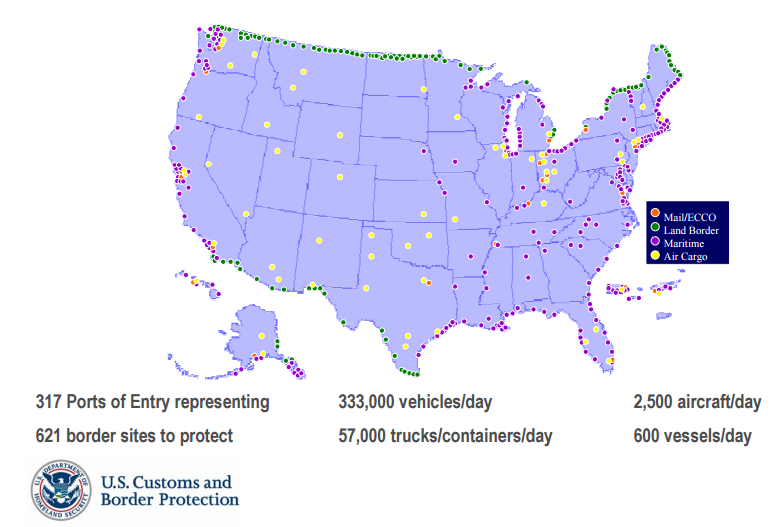
\includegraphics[trim = 0cm 0cm 0cm 0cm, clip,scale=0.55]{./figures/RPM_map.png}
   \caption{CBP plan for RPM deployment \cite{Simmons2005}.}
     \label{fig:RPM_map}
\end{figure}



The CPB/AAPA RPM plan outlines a phased implementation approach targeting locations around the U.S. based on their assessed risk. The plan additionally details collaboration with the Pacific Northwest National Lab, which is responsible for the development of cutting-edge, harmless, and passive detection systems (illustrated in \autoref{fig:RPM_designs}). In 2005, RPM systems had already been deployed at 14 terminals, with another 18 in construction, and 27 in final design \cite{Simmons2005}.


\begin{figure}
        \centering
        \begin{subfigure}[b]{0.3\textwidth}
                
\includegraphics[width=\textwidth,scale=1]{./figures/fixed_vehicle.png}
                \caption{Fixed  vehicle monitor.}
                \label{fig:fixed_vehicle}
        \end{subfigure}%
        ~ %add desired spacing between images, e. g. ~, \quad, \qquad, \hfill etc.
          %(or a blank line to force the subfigure onto a new line)
        \begin{subfigure}[b]{0.3\textwidth}
                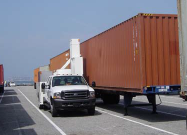
\includegraphics[width=\textwidth,scale=1]{./figures/mobile_cargo.png}
                \caption{Mobile cargo monitor.}
                \label{fig:mobile_cargo}
        \end{subfigure}
        ~ %add desired spacing between images, e. g. ~, \quad, \qquad, \hfill etc.
          %(or a blank line to force the subfigure onto a new line)
        \begin{subfigure}[b]{0.3\textwidth}
                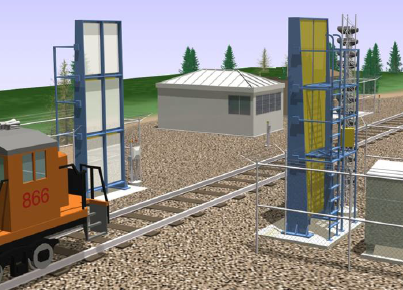
\includegraphics[width=\textwidth,scale=1]{./figures/perm_train.png}
                \caption{Fixed train monitor.}
                \label{fig:perm_train}
        \end{subfigure}
        \caption{RPM designs and examples \cite{Simmons2005}.}\label{fig:RPM_designs}
\end{figure}
  




  

Eight years after the initial development of the RPM plan, the Office of the Inspector General published a report documenting the progress made in the RPM development with an emphasis on seaports \cite{DepartmentofHomelandSecurityDHS2013}. The document reports 444 active RPMs screening 99\% of inbound containerized cargo at large seaports, with the other 1\% of cargo entering low-volume seaports (this 1\% is presumably not monitored). 
One point of concern outlined in the report is that many RPM devices (up to 10\% at a large port) were no longer being used. Further, given the limited use of funds for the DNDO and CBP, no plans (as of the report in 2013) were put in place to ensure continued use of RPM technology. Recommendations were generated in the report to develop an organization to ensure the continued and efficient use of RPMs at seaports. 

Development of advanced RPM technologies (meant to replace the old devices) has been continued in recent years, although not necessarily with great success. In 2013, the Government Accountability Office released a report outlining the technical failure of the development of Advanced Spectroscopic Portal Monitors (ASPs) \cite{UnitedStatesGovernmentAccountabilityOffice2013}. Lessons were outlined and documented from the failed attempt at replacement RPMs, but years after the final technology tests. Overall, the entire process was quite cumbersome and ineffective. 

In order for the U.S. to be effectively guarded against potential nuclear threats from non-state actors such as ISIL, a streamlined approach must be taken to portal and border monitoring. While the initial development and deployment of RPM technology seems to have been fairly effective based on unclassified reports, the caveat to these programs is their reported deterioration over a decade of dormancy \cite{Simmons2005,DepartmentofHomelandSecurityDHS2013}. 

This document suggests the aggressive continued advancement of such programs. The continued development of new technologies, as outlined in \autoref{app:tech}, must be exploited for every feasible advancement that can lead to increases in national security. This document suggests a priority-phased plan outlining a strong technological collaboration with government labs, similar to the plan put forth in 2005, in order to develop and deploy the next generation of RPMs \cite{Simmons2005}. Such a plan would be managed by the DNDO and executed by the CPB and AAPA. This plan, however, can only be effective given the successfully executed deployment of any developing technology. Technological failures such as the ASP development program are acceptable so long as workable alternatives exist. 



\section{Second Line of Defense}

If ISIL attempts to move a nuclear device once they obtain it, it is possible that the device may be transported on boats. This may allow for detection of the device at port entries. Given the Second Line of Defense's radiation detection equipment at borders, airports, and strategic feeder ports in Russia, former Soviet Union states, and other key countries, the current capabilities of the U.S. NNSA SLD Core Program, described in \autoref{sec:Trafficking}, could be modified to limit ISIL's ability to smuggle a nuclear weapon out of its territory \cite{Kilmartin2010}. The same proposed changes to stem the inflow of nuclear materials into ISIL controlled territory would apply here as well. The addition of the Port of Lattakia and the Port of Tartous (see \autoref{fig:seaports}) reduces the threat of overseas delivery of a nuclear weapon.   



\section{Protection of U.S. Assets Abroad}

\subsection{Force Protection}

While interception of the shipment would be preferred as discussed in the previous sections, it is not guaranteed, and a layered approach to defense is preferred.  If ISIL does acquire a nuclear weapon or RDD, they will most likely target sites overseas since it is unlikely they will acquire a long range delivery system and long distance transportation to the U.S. will be difficult, if not impossible (See \autoref{sec:domestic_protection}).  For this reason, the area around ISIL territories are high risk target areas.  It must be assumed that any American military bases or ships in these regions could be chosen as a target by ISIL.  Since protecting Americans in this region is the top priority, these bases must be prepared for a possible nuclear or radiological attack.  The current protective measures for the military overseas will be analyzed and updated to protect against a nuclear or radiological threat from ISIL.

On October 2, 2006, the Department of Defense issued Instruction 2000.16, which introduced the Force Protection Condition (FPCON) system.  FPCON is the Department of Defense's official terrorist threat system that identifies the possibility of an attack against a military facility or ship.  It also recommends preventive actions and responses that should be taken by military facilities and ships depending on the threat level.  The FPCON threat level is determined by military intelligence on the likelihood of a terrorist attack and is normally set by the geographical combatant commander for that region \cite{Usd2006}.  Jurisdiction of the Middle East falls under the USCENTCOM Combatant Commander.  Since the FPCON system was set up to be used by any U.S. military installation in the world, if intelligence indicates ISIL has acquired a weapon, it is important that this is communicated to all of the geographical combatant commanders.  However, the highest priority should be placed on communicating this intelligence to the USCENTCOM Combatant Commander so that the appropriate FPCON measures can be taken.

The FPCON system has not changed much since it was issued.  It was supplemented by Instruction 2000.12, which was issued on March 1, 2012 and talks about the DoD Antiterrorism Program \cite{U.S.DepartmentofDefense2013}.  However, it does not significantly change the protective measures assigned by FPCON.  Currently, the FPCON consists of five progressive levels of increasing protective measures.  The levels are FPCON Normal, FPCON Alpha, FPCON Bravo, FPCON Charlie, and FPCON Delta.  FPCON Normal is the lowest threat level which all domestic and foreign bases must remain at all times at the minimum.  Since there is always a global threat of possible terrorist activity, minimum security measures must always be taken, such as routine security posture and access control to the installation.  The next threat level is FPCON Alpha, and it applies when there is an increased threat of terrorist activity against the installation.  The extent and nature of the threat may still be unpredictable.  The measures taken under FPCON Alpha must be possible to maintain indefinitely.  FPCON Bravo applies when the threat of terrorist activity increases and becomes more predictable.  Unlike the FPCON Alpha level, a prolonged period of maintaining FPCON Bravo may affect the operational capabilities of the facility and the relationships with local authorities.  The next level, FPCON Charlie, applies when a terrorist incident occurs or military intelligence indicates that a terrorist action or targeting against some facility is likely.  Maintaining this level for a prolonged period may create hardships and affect activities of the personnel.  The highest level is FPCON Delta.  This level only applies in the immediate area where a terrorist activity has occurred or intelligence indicates that a terrorist attack on that particular facility or ship is imminent.  This level is usually localized only to the applicable facility or ship instead of all bases in a region.  These measures are not intended to be sustained for an extended duration as it essentially shuts down the facility except for protective measures \cite{Usd2006}.

If ISIL acquires nuclear weapons, all military bases in the region around ISIL territory should be placed on FPCON Charlie unless intelligence indicates an imminent threat to a particular facility.  Under Charlie, the facility still needs to run, except with much stricter security measures.  Access to the facility or ship will be limited to only a few entrances with random vehicle searches.  The identity of every visitor must be verified, and there will be random searches of their personal items, such as suitcases, briefcases or packages, as well.  There will also be increased patrols of the facility and possibly the perimeter surrounding the facility with assistance from local authorities.  If possible, public and military roads and public facilities around the perimeter of the base will be closed.  Ships also have some additional measures taken under FPCON Charlie.  Even at FPCON Alpha, in a foreign port, the minimum standoff distance from a Navy ship is 400 feet.  However, under FPCON Charlie, there are also frequent and random searches of the pier.  All public visits are terminated, unauthorized crafts are kept away from the ship, unnecessary vehicles are blocked from entering the port, and if possible, a small boat exclusion zone is established around the ship \cite{Usd2006}. 

Even stricter measures are implemented under FPCON Delta as it completely locks down the base or ship when the threat is imminent.  FPCON Delta will only be used if the weapon is detected near a particular ship or base or intelligence indicates ISIL plans on attacking that particular facility or ship.  Under FPCON Delta, all vehicles and their contents will be searched before they can enter the facility.  All personnel entering the base must be positively identified, and all of their personally carried items must be searched without exception.  There will be frequent checks of the exterior of buildings and of parking lots in the base.  All non-essential movement will be restricted.  If not done already and if possible, all public and military roads and facilities will be closed around the perimeter of the base.  At the very least, the military road allowing access to the facility must be closed.  For a ship, only necessary personnel will be permitted topside of the ship and all necessary weapons for defense will be employed.  If possible, the ship will cancel its port visit and leave the port \cite{Usd2006}.

Unfortunately, all of these measures were designed to protect against a conventional or possibly chemical or biological terrorist attack.  They were not planned with nuclear weapons or RDDs in mind.  For this reason, it is this policy's recommendation that additional security measures are added.  For the currently established inspections and searches at these higher threat levels, handheld radiation detection devices should be standard equipment.  The detection devices should be used in conjunction with conventional search methods to search the personal belongings and vehicle of anyone trying to enter the facility. They should also be used for inspections on base.  Also, it may be necessary to have modified FPCON Charlie and Delta levels in case of nuclear attacks as well as the regular threat level measures for a non-nuclear threat.  The measures necessary for a nuclear attack will be unnecessary and somewhat impractical to implement just for a conventional terrorist attack.  So, there should be modified measures in the special case of a nuclear threat.  First, for the modified FPCON Charlie, the restrictions outside of the base should be increased.  It is assumed that if ISIL acquires a weapon, it will be small yield.  According to the Federation of American Scientists, Pakistan was only able to first develop bombs with a maximum yield of about 12 kilotons \cite{FederationofAmericanScientists2002}.  If ISIL develops their own bomb, it is unlikely they will develop as large of a bomb as Pakistan, and if ISIL acquires a bomb through Pakistan or North Korea, it will likely still be a small yield device.  For this reason, if possible, every road and facility that is within a 1 to 1.5 mile radius of the base should be closed.  This will severely minimize the damage to the base if the weapon is detonated outside of this perimeter.  Also, if possible, for ships, the pier should be closed to the public and all non-necessary personnel.  The standoff distance from the ship should be increased to 1 to 1.5 miles as well for the modified FPCON Charlie.  For the modified FPCON Delta, it is assumed that the base will be attacked by a nuclear weapon or RDD.  Hardened bunkers should be constructed, if they do not already exist, before ISIL develops a weapon.  Regular FPCON Delta measures will be followed, but, additionally, all civilian and non-essential personnel should move to these nuclear bunkers.  For ships, the ship should just follow regular FPCON Delta measures and leave the port as soon as possible.  These additional security measures should hopefully minimize the damage and probability of a nuclear attack on a military base in the region.








\section{Weaponization \& Delivery}

If ISIL is able to obtain a nuclear weapon, the next steps for them would be to develop a method of delivery, pick a target, and deploy and detonate the bomb.  If possible, the first priority of the U.S. should be to locate where ISIL is storing the bomb and destroy it using drone strikes.  However, it is highly improbable that the exact location of the bomb will be known or found using current detection technologies.  Even if it is found, it might be stored underground where drone strikes would not reach it.  Therefore, the more practical strategy for the U.S. will be to try to stop ISIL at each of the previously mentioned steps.   First, the U.S. will need to determine what delivery methods are possible for ISIL.  


The associated non-nuclear delivery technologies are also significant proliferation risks from states with the developed capabilities, if not more significant due to less oversight from international organizations and control regimes coupled with a higher degree of technology proliferation. Relevant delivery systems for WMD ISIL may consider include ICBMs, cruise missiles, and gravity bombs. 

There are more than thirty countries now capable of domestically producing ballistic or cruise missiles, including North Korea and to a lesser extent Iran \cite{U.S.CongressOfficeofTechnology1993}. Despite the increasing risk of proliferation of delivery systems for WMD, there is no binding international nonproliferation treaty that controls the spread of missiles or other delivery systems. There are two major examples of regimes that work to limit the proliferation of WMD delivery systems. The Missile Technology Control Regime is an informal and voluntary association of countries that work together to limit the proliferation of unmanned WMD delivery systems. The 2002 Hague Code of Conduct against Ballistic Missile Proliferation contains a set of general principles that its subscriber states pledge to follow. Neither of these sets of rules are binding, and neither include the states of most concern: North Korea, Pakistan, India, and Iran.

Cruise missiles, due to their simpler designs and lower costs, are more widely proliferated. Many cruise missile designs specifically avoid export controls specified by the Missile Technology Control Regime. The combination of \enquote{over-the-counter} technology, high probability of defense penetration in supersonic cruise missiles, and a relatively low barrier to technology development make cruise missiles ideal for initial acquisition followed by indigenous development and use \cite{OfficeoftheUnderSecretaryofDefenseforAcquisitionandTechnology1998}. 

The simplest delivery system is a combat fixed-wing aircraft coupled with a gravity bomb package. It is generally assumed most states seeking WMD already possess aircraft or can purchase them in international markets, and this assumption holds true for ISIL as well. Manned aircraft represent the most probable and delivery system for a WMD. 

The most probable path for ISIL to acquire a WMD delivery system would be to purchase or steal fixed-wing aircraft. This option is the easiest to achieve and most flexible, although the most vulnerable to disruption mid-delivery. However, a second and possibly more realistic use of nuclear materials by ISIL would be a RDD \cite{D.Esfandiary2014}. Delivery systems for RDDs are not limited to the traditional set discussed above, and small yield or compact designs can even be hand-carried to the target. The use of RDDs does not require the delivery systems discussed and nullifies arguments for delivery systems control. 


The U.S. can prevent ISIL from acquiring the necessary components to build more complex delivery system and slow down movement of the bomb.  Then, the U.S. can make predictions about the group's targets based on geographical location from ISIL and try to intercept the bomb before it reaches the target.  

\section{Post-Detonation U.S. Response}

If ISIL is successful in detonating a nuclear device, the U.S. must be prepared to take military action in response, as well as to prevent the detonation of a second device. Depending on the U.S. assessment of the threat posed by ISIL's attack (which is a discussion that must be had at the highest levels), a military response may range from an increased air campaign to U.S. ground force involvement in a campaign to destroy ISIL. Additionally, the U.S. must be prepared to collect forensic data to determine, if possible, if any additional countries were complicit in ISIL acquiring a nuclear device. If another nation aided ISIL, the U.S. should consider military action in response consistent with the recommended declaratory policy in \autoref{sec:purchase_gift}.



\chapter{Dissenting Opinion}


\begin{center}
 \enquote{One of the most important lessons of the Cold War was that incessantly worrying about the low-probability/high-impact cases was a mistake.}  - Kenneth Pollack \cite{pollack2014unthinkable}
\end{center}


The ISIL nuclear threat is, by definition, a low-probability/high-impact case as this report has shown. As Pollack points out, historically the low-probability/high-impact events receive a disproportionate amount of the national attention and funding \cite{pollack2014unthinkable}. Americans in particular are susceptible to the allure of these \enquote{grand challenges} and often pour massive amounts of monetary and human resources into developing solutions, but the U.S. is certainly not alone in this regard. Staying within the nuclear realm, both the U.S. and U.S.S.R. both devoted significant attention to the \enquote{bolt from the blue} problem during the Cold War, despite there never being evidence that such a tactic was considered or likely to succeed \cite{pollack2014unthinkable,Bracken2013}.  In fact, some of this planning still takes placed even today, despite 20+ years passing since the end of the Cold War.

In addition to the inefficient use of government resources, the focus on rare events can lead to the misinterpretation of signals and an exacerbation of the original dominant security risk.  For example, the U.S.S.R interpreted the 1983 Able Archer NATO nuclear exercise as being a preparation for a \enquote{bolt from the blue} attack \cite{pollack2014unthinkable}. As applied to ISIL, the remote threat of nuclear terrorism can serve as a distractor from the actual security risks posed by ISIL to U.S. interests in the region.  Additionally, it would result in less resources and political capital to devote to addressing the economic, political, and human rights issues that gives rise to ISIL and similar movements throughout the Middle East in the first place \cite{Morand2015}. Unintentional second-order consequences could result in the U.S. and international focus on nuclear terrorism issue creating the environment, public awareness and making a nuclear capable ISIL credible, for ISIL to achieve its goals through propaganda without actually developing nuclear capabilities.  For example, while not well orchestrated by ISIL standards and reported to an unbelieving public, there have been previous overstated reports of ISIL's nuclear capabilities \cite{Bunn2014}.  In the future, it may be hard to tell fact from fiction or to prove a negative to a skeptical American public.  While this strategy could backfire on ISIL, most notably through the deployment of U.S. forces to combat the threat, a more likely result under the current Administration is that the U.S. would seek diplomatic and technical solutions.  

In fact, diplomatic and technical solutions are the bulk of the policy proposals put forth in this report.  In theory, this is a great approach as it would not be difficult to influence the American people or U.S. government to support efforts to combat terrorism, nuclear or non-nuclear, in the post-9/11 environment. Since 9/11, the U.S. has largely adopted a \enquote{1\% Doctrine} where all threats with even a 1\% likelihood should be eliminated \cite{pollack2014unthinkable}. This, coupled with a general reluctance of the American populace to question the U.S. military or anything posed as a national security issue, has given de facto carte blanche to all \enquote{good idea fairies} to promote their particular product or idea in the name of improving national security \cite{Fallows2015}. A relevant example to the proposed policies in this report is the history and effectiveness of radiation portal monitors and the Advance Spectroscopic Portals.

RPMs evolved out of a layered defense concept to prevent a low-probability/high-impact scenario, nuclear terrorism. This layered defense is composed of RPMs as discussed in \autoref{sec:domestic_protection}, the overseas equivalent known as the SLD as discussed in \autoref{sec:Trafficking}, and the Global Threat Reduction Initiative discussed in \autoref{sec:GTRI}.  Despite the layered technical and diplomatic approach, there are significant gaps in the ability to intercept a shipment into the U.S. containing SNM.  For example, DHS has implemented 99\% screening at seaports, but struggles to implement a significant screening at airports, due to a lack of natural choke points and disruption caused by screenings, and at the U.S.'s notoriously porous border crossings \cite{DepartmentofHomelandSecurityDHS2013,GovernmentAccountabilityOffice2012}.  Even if a shipment does cross a border, seaport, or airport with a RPM, the detection probability is only 90\% in the best of scenarios, if the RPM is even operational at the time \cite{DepartmentofHomelandSecurityDHS2013,DepartmentofHomelandSecurityDHS2006}.  To top of the list of issues, the ANSI standard for certification of RPMs contains no SNM requirements due to the inherent difficult in passive detection of SNM \cite{Ansi2007}.  The ASP program was conceived to address some of these problems and increase interception through advanced detectors and algorithms, but it failed to pass 6 of 10 criteria in field tests, criteria which were widely criticized as being favorable to the vendors in the first place \cite{UnitedStatesGovernmentAccountabilityOffice2013}. To further complication matters, if a competent proliferator uses shielding or naturally occurring radioactive material within the shipment, it is effectively impossible to pull out the SNM signal with the passive detection systems currently employed without generating significant false positives \cite{UnitedStatesGovernmentAccountabilityOffice2013,UnitedStatesCongress.House.CommitteeonHomelandSecurity.SubcommitteeonEmergingThreatsCybersecurity2007}.  Nonetheless, DNDO continues to invest significant effort into a technical solution that is at best 90\% effective, and at worst almost useless, with the goal of deterring an extremely low probability event.  The proposed policies in this report follow that same trend and fail to learn the lessons of history in this regard.      

While avoiding unintended consequences or wasted resources are compelling reasons to reconsider the proposed policies, perhaps the most compelling reason is to place the threat and proposed policies into context.  It is perhaps a bit generous to even call ISIL obtaining a nuclear weapon a low probability event as there is zero basis in history for it to be able to do so \cite{pollack2014unthinkable,Bracken2013,Nacht1867,Reed2010,Agency2004}. Developing nuclear weapons amidst crippling sanctions, airstrikes, and a dedicated opposition has never been done, despite several nation states attempting to do so \cite{Reed2010,Agency2004}.  In fact, the only nation to develop a nuclear weapon in the time of war was the U.S., and the U.S. mainland was never seriously threatened. Supposing that ISIL was the proverbial \enquote{Black Swan} case, it is worth noting that, with the exception of the U.S., no state has gone from decision to having a deliverable nuclear weapon in under four years \cite{Reed2010}. Even modern conservative estimates place the timeline at 5-6 years for a competent nation state pursuing an optimal path to a nuclear weapon \cite{Harney2006}. Proponents of the threat of nuclear terrorism will likely point to the possibility that ISIL will circumvent the indigenous development route completely and pursue theft or purchase of key components or a complete device.  Again, there is no history to suggest that a nation state would take that risk given the enormous repercussions it would face \cite{pollack2014unthinkable}.  Additionally, anything short of a complete device would still require significant development to weaponized, perhaps three to four years depending on the amount of assistance ISIL received \cite{Harney2006}.  

The sum result of this discussion is that we are at best facing the prospect of a nuclear armed ISIL in several years assuming no disruptions due to discovery and outside assistance from a nuclear capable state, both of which are counter to the history of every nuclear program \cite{pollack2014unthinkable,Reed2010}.  Given this fact, the best policy we have is to place financial, diplomatic, and military pressure on ISIL, all of which are current policies of the Obama Administration as shown in \autoref{fig:policy_chart}.  Additionally, there are no identified potential proliferation pathways that are not covered to some extent by current policies, programs, or operations.  As war was building in Europe in 1940, Edward Murrow reported, \enquote{The people here feel the machine is out of control, that we are all passengers on an express train traveling at high speed through a dark tunnel toward an unknown destiny.  The suspicion recurs that the train may have no engineer.}  The proposed policies are emblematic of a machine out of control in support of Dick Cheney's \enquote{1\% Doctrine.} Therefore, the dissenting opinion recognizes that the marginal cost to implement the proposed policies outweigh the marginal benefit and recommends to not repeat the mistakes of history by implementing the proposed policies of this report. Instead, it is proposed that the U.S. implements no changes to U.S. policy specifically to prevent the low probability event that is ISIL obtaining nuclear weapons. This would entail \enquote{staying the course} with President Obama's current policy of disrupting, degrading, and ultimately destroying ISIL as a necessary and sufficient condition to prevent nuclear weapon acquisition, while not losing focus on the real ISIL national security challenges \cite{WhiteHouse2014}.



% \chapter{???????  Do final consistency checks for ISIS/ISIL, US/U.S., apostrophes, SLD/SLoD, quote marks  ???????????}



% \chapter{???????  Redo captions, to have true-ordered caption citation numbers    ?????????}





\chapter{Conclusions \& Suggestions}

Though the probability of ISIL acquiring nuclear weapons, a radiological dispersal device, or special nuclear material may be small, it is not zero. If ISIL indeed acquired any of these through the possible pathways outlined in this report (or otherwise), the consequences would be dire. 

This report has illustrated the details of policy recommendations focused on preventing the low-probability / high-consequence event of ISIL becoming a nuclear threat. To target all possible pathways, this report has made policy recommendations - new ones, as well as additions to existing policy - in an effort to prevent weapons theft or purchase, the strengthening of ISIL foundational capabilities for indigenous development, or the acquisition of radiological material for use in a radiological dispersal device. These policies are  summarized here:

\begin{easylist}[enumerate]
& Policies specifically targeting \textbf{indigenous development:}
&& Targeting of foundational capabilities	
&&& Income 
&&& People and expertise 
&&& Infrastructure
&& IAEA monitoring 
&&& Additional Protocol – push for more signatures 
&&& International and Trafficking Database – push for increased cooperation
& Policies specifically targeting \textbf{proliferation through theft/purchase:}
&& IAEA monitoring 
&&& International and Trafficking Database – push for increased cooperation
&&& Additional Protocol – push for more signatures 
&& Global Threat Reduction Initiative (GTRI) 
&&& Push for the cooperation of more nations
&& Strengthening of multilateral security agreements
&& Nuclear Forensics Attribution Act (NFAA)
&&& Explicit declaratory policies, explicit deterrence 
&& United Nations Security Council Resolution (UNSCR) 1540 
&&& Additional provisions and security expert group
&& Second Line of Defense (SLD)
&&& Additional foreign ports
& Policies specifically targeting \textbf{delivery/staging:}
&& Military Force Protection Condition (FPCON)
&&& Increased military base safety
&& Advanced Radiation Portal Monitor (RPM) Plan
&&& Increased domestic port monitoring and advanced monitor development
&& Second Line of Defense (SLD)
&&& Monitor additional foreign ports
\end{easylist}


As with the development of any policy, decisions are based on tradeoffs. It is important to understand the nature of diminishing returns when targeting efforts and funds to prevent an ISIL nuclear threat. This is true not only for crafting US policy, but also for understanding the intentions and motivations of ISIL and assessing the probability of their efforts to acquire nuclear material or devices. It is imperative to match U.S. policy with an understanding of the likelihood that ISIL will pursue one or more of these possible nuclear routes.

Furthermore, the caveats in implementing these policies must be understood. The realization of some of the policy recommendations might be diplomatically difficult in light of current political relationships, keeping in mind nuclear cooperation agreements (or lack thereof) with other countries, and the relationships between states relevant to this conflict. It is important to continue to encourage the recognition of the diplomatic difficulty in the policymaking and recommendation process.

The recommendations that have been illustrated in this report rest on the assumption that a nuclear ISIL needs to be prevented at any cost. A dissenting viewpoint has been offered and explored, and recommends focusing efforts on dismantling ISIL as a movement instead of dedicating disproportionate resources to an unknown probability of nuclear acquisition. Regardless of the philosophy on how to allocate funding to implement policy options, it is at the very least prudent to spend efforts on reducing knowledge uncertainty of possible ISIL-related nuclear event. Part of the low-hanging fruit of increasing preparedness and U.S. response capability (especially keeping in mind the cost, feasibility, and tradeoffs of policy implementation) is the assessment of possible nuclear outcomes, such as this report has done. However large or small the perceived risk, the work contained in this report contributes to the knowledge of prevention and response to the possibility of a nuclear ISIL.

Although the discussion about the allocation of efforts continues among policymakers, the Obama administration's National Security Strategy in 2010 has strongly stated its position: \enquote{This Administration has no greater responsibility than the safety and security of the American people. And there is no greater threat to the American people than weapons of mass destruction, particularly the danger posed by the pursuit of nuclear weapons by violent extremists and their proliferation to additional states} \cite{Obama2010}. The work in this report supports the national security goals of the current administration if the recommended strategies are implemented.



% \section{??????? ORDERED LIST OF RECOMMENDATIONS HERE ????????}






\appendix
\chapter[Appendix A: Glossary of Nuclear Terminology]{Glossary of Nuclear Terminology}  \label{app:glossary}



\textit{Note: All terminology is taken from the U.S. Nuclear Regulatory Commission  \cite{USNRC2015}.}

\textbf{Radioactive Decay:} The spontaneous transformation of one radioisotope into one or more different isotopes. The isotopes created may or may not also be radioactive. Radioactive decay may also be used to refer to the emission of a gamma ray or a conversion electron emission, which reduces the energy of the decaying isotope but does not change its identity. 

\textbf{Alpha Radiation:} The radioactive decay of a nuclide which results in the emission of a \ce{^{4}He} atom. Alpha radiation is sometimes followed by gamma emission. 

\textbf{Beta Radiation:} A radioactive decay of a nuclide which results in the emission of an electron and an electron antineutrino pair, or a positron and an electron neutrino pair. 

\textbf{Fusion:} A nuclear reaction in which atomic nuclei of low atomic number merge and become a heavier nucleus, thereby releasing energy. 

\textbf{Special Nuclear Material:} Plutonium, \ce{^{233}U},  or \ce{^{235}U}.

\textbf{Gamma Radiation:} A radioactive decay which results in the emission of a high energy- short-wavelength, electromagnetic radiation emitted from within the nucleus of an atom. Gamma radiation often follows the emission of an alpha or beta particle, and always follows a fission event. 

\textbf{Electron Volt (eV):} A unit of energy equivalent to the work required to accelerate an electron through a potential difference of 1 volt. 

\textbf{Fission:} The splitting of an atom, which releases energy. During fission, a heavy (large A) nucleus splits into two or three smaller nuclei and emits gamma rays and neutrons. 

\textbf{Nuclide:} A distinct nucleus, defined by the total number of neutrons and protons contained therein.  

\textbf{Fast Neutron:} A neutron with kinetic energy in excess of 1.5 MeV.

\textbf{Thermal Neutron:} A neutron which is in thermal equilibrium with its surroundings. 

\textbf{Fissile Material:} A nuclide that is capable of undergoing fission after capturing thermal neutrons.

\textbf{Fissionable Material:} A nuclide that is capable of undergoing fission after capturing a fast or thermal neutron.



\chapter[Appendix B: Basic Nuclear Physics \& Definitions]{Basic Nuclear Physics \& Definitions}  \label{app:physics}



\section{Nuclear Structure}

Atoms are essentially a dense core of protons and neutrons surrounded by an electron cloud. The neutrons and protons in the nucleus (atomic core) are also known as nucleons, collectively \cite{krane1987introductory}. For the purposes of this report, a complete understanding of the atomic structure is not necessary. However, what should be understood is the difference between an element and an isotope, and how to determine what element and isotope an atom is based on its nuclear composition. 

Within the nucleus, the number of protons (Z) defines what element an atom is. For example, an atom with six protons is a carbon atom, and an atom with ninety two protons is a uranium atom. The number of total nucleons (A), or the number of protons and neutrons combined, defines the isotope of the element that the atom is \cite{krane1987introductory}. For example, a carbon atom with six neutrons has twelve nucleons, and is known as a \ce{^{12}C} atom. A uranium atom with one hundred and forty three neutrons has two hundred and thirty five nucleons, and is known as \ce{^{235}U}, an important element in nuclear science and for many nuclear weapons. It is interesting to note that different isotopes of the same element can behave significantly differently. An excellent example of this is that \ce{^{235}U} readily fissions in nuclear reactors and weapons, but \ce{^{238}U} only reliably fissions under specific conditions, and therefore is not a useful fuel in nuclear weapons \cite{krane1987introductory,Duderstadt1976}. 


\section{Fission}

Nuclear fission is the process in which a nucleus splits into two nuclei of roughly equal mass \cite{krane1987introductory,Lamarsh2013}. This is the dominant reaction in nuclear weapons that produces the incredible amount of energy released upon detonation. The two isotopes used in fission-based systems as fuel are \ce{^{235}U} and \ce{^{239}Pu}. These fuel isotopes are used individually in a single weapon, not as a mixture. In weapons, neutrons are used to begin the fission process in nuclei, which when they fission also release excess neutrons, which go on to spark further fission reactions. This is known as the fission chain reaction. Controlling this chain reaction is the business of nuclear reactors, while accelerating it as much as possible is the purpose of a nuclear weapon \cite{Duderstadt1976}. 

It is also important to understand that the two fuel isotopes are not naturally found in forms that can be directly used to fuel a nuclear weapon \cite{Benedict1981,Lewis2008}. Instead, \ce{^{235}U} is found in extremely small amounts in natural uranium deposits and must be further enriched and concentrated for use in a weapon. \ce{^{239}Pu}, on the other hand, is not naturally occurring and must be produced in a nuclear reactor specially designed for this purpose. Because of this, \ce{^{235}U} is the easier to acquire and use of the two fuel isotopes, and thus is of more concern. 




A fission reactor or device operates on the principle that fissile materials (list of materials) will undergo fission when stuck by neutrons of sufficient kinetic energy. A nuclide which undergoes fission will release between 100-200 MeV in addition to 2-3 neutrons, which may be utilized to cause subsequent fissions in other fissile nuclei \cite{krane1987introductory}. The minimum amount of fissile material needed in order to sustain a chain reaction is known as the critical mass, which depends on the type, density, and shape of material used. A tamper, which is a high Z material which acts as a neutron reflector, is typically used in order to reduce the critical mass. 

\section{Criticality}

Criticality in a system is defined as the state in which the rate of reactions in the system is constant, producing a constant energy output over time. In a fission system, criticality is a constant rate of fission reactions over time, and is also known as a controlled fission reaction \cite{Duderstadt1976}. This is the dominant operating state of nuclear reactors that maintain a constant power level during the majority of their operational lives \cite{Ott1983}. A supercritical system is a system where the reaction rate is constantly increasing, and a subcritical system is thus a system where the reaction rate is constantly decreasing. 

Clearly, it is important to understand that nuclear weapons rely upon the fact that their nuclear fuel can be arranged in such a way that it becomes violently supercritical when the user specifies, and not before \cite{Lewis2008}. Therefore, in terms of criticality, it can be said that the nuclear core of a weapon is initially subcritical before detonation, and  is rendered highly supercritical at the exact moment of detonation. This is fundamentally what allows the weapon to release such earth-shaking amounts of energy nearly instantly when it is used, but to be stored safely before then \cite{Prussin2014,Defense1998}. 


\section{Critical Mass}

The minimum amount of special nuclear material needed to produce the critical core of a  fission weapon is called the critical mass. This value can depend on many different features including isotope, geometry of the material, micro-structure of the material, and device design. Given the many variables in play it would be infeasible to include the critical mass of every possible weapons configuration here. However, to give a general idea, \autoref{tab:critical_mass} presents the critical mass of two different designs for several types of weapons. Additionally the yields of fission devices can vary based on many factors including, type of material, device design, amount, efficiency, and many other factors. Yields are typically on the order of kilotons \cite{Moody2014}. 


\begin{table}
\centering
\begin{tabular}{|l|c|c|}
\hline
\multicolumn{1}{|c|}{Material}                                              & Critical Mass, Bare Sphere (kg) & Fully Tampered Sphere (kg) \\ \hline
\ce{^{235}U}                                                                       & 52                              & 17                    \\ \hline
\ce{^{239}Pu} (alpha phase)                                                        & 10                              & 4                     \\ \hline
\ce{^{239}Pu} (delta phase)                                                        & 16                              & 6                     \\ \hline
\begin{tabular}[c]{@{}l@{}}Reactor Grade Pu \\(60\% enriched in \ce{^{239}Pu})\end{tabular} & 13                              & -                     \\ \hline
\ce{^{233}U}                                                                      & 15                              & 6                     \\ \hline
\end{tabular}
\caption{Critical Masses of a Bare and Fully Tampered Sphere for Various Special Nuclear Materials \cite{Moody2014} }
\label{tab:critical_mass}
\end{table}





\section{Fusion}

Fusion is fundamentally the inverse process of fission. Fusion is the process wherein two light nuclei combine to form a single, heavier nucleus, and in doing so release a large amount of energy, possibly in addition to neutrons or various charged particles \cite{krane1987introductory,Dolan1982}. In thermonuclear weapons, fusion is typically used to \enquote{boost} the total energy production of a weapon significantly beyond the release otherwise achieved through fission alone. Fundamentally, the fusion reaction provides a large initial supply of neutrons that allows the fission process to begin at a much higher rate than it could alone \cite{Prussin2014}. 

\section{Energy Release}

Typical nuclear reactions release energies on the order of 1-10 MeV \cite{Prussin2014}. In comparison, typical chemical reactions release energy on the order of a single eV per molecule, and perfectly combusted TNT, a common high-explosive, releases approximately 35 eV per molecule \cite{Prussin2014}. Clearly the amount of energy released in nuclear reactions is many orders of magnitude greater than typical chemical reactions more familiar to society. However, the energy released in fission, the primary nuclear reaction in nuclear weapons, is 100 times that of typical nuclear reactions (approximately 180 MeV per reaction) \cite{krane1987introductory,Loveland2005}. Combining the incredible energy released per fission reaction with the density of the fuel in nuclear weapons, it becomes readily apparent that nuclear weapons contain an energy source greater than any other on earth. Combined  with the incredibly short timescales on which nuclear reactions occur (on the order of 10\(^{-7}\) s - 10\(^{-6}\) s),  nuclear weapons become tools of unimaginable power and destruction \cite{Loveland2005,Cochran1994,Prussin2015}.  


\section{Radioactive Decay}

For all elements, there are isotopes which are not naturally occurring. The reason that these isotopes are not observed in nature is that they are radioactive. A radioactive isotope, due to is structure, is energetically unstable, to the point that it will emit excess nucleons or energy to become stable \cite{Loveland2005}. This process of reaching a more stable nuclear structure is known as radioactive decay. The three most common modes of radioactive decay are referred to as alpha (\(\alpha\)) decay, beta (\(\beta\)) decay, and gamma (\(\gamma\)) decay \cite{Loveland2005}. In general, isotopes that are very energetically unstable decay faster and with greater releases of energy, whereas isotopes that are not far from stability decay more slowly and with lower-energy releases. This makes very unstable isotopes very dangerous; less unstable isotopes are less of a radiation hazard \cite{krane1987introductory}.

Alpha and beta decay change the structure of the nucleus of the atom, by emitting or transforming excess nucleons to stabilize the nucleus. The change in the nucleus' structure literally changes it into a different element altogether \cite{krane1987introductory}. Alpha decay allows heavy (A \textgreater \(\approx\) 110) nuclei to stabilize themselves by shedding excess nuclei. In alpha decay, the nucleus emits an \(\alpha\) particle, also known as the nucleus of a \ce{^{4}He} atom. This particle is composed of two protons and two neurons, and typically has a kinetic energy of 4 - 10 MeV \cite{krane1987introductory}. 

Beta decay allows nuclei with an excess of either protons or neutrons to stabilize themselves by transforming an excess proton into a neutron, or vice-versa, releasing a neutrino in the process \cite{krane1987introductory}. In beta decay,  the nucleus emits a \(\beta\) particle, which is either an electron, or its positively-charged counterpart, the positron. \(\beta\) particles typically have a kinetic energy of several hundred keV;   the electron's kinetic energy varies, with an average of 1/3 of the maximum electron energy, while the remaining energy is carried off by a nearly undetectable electron antineutrino \cite{krane1987introductory}.

Gamma decay allows nuclei with a high-energy internal configuration of their nucleons to stabilize by shifting that configuration to one lower in energy. The extra energy is released in the form of a high-energy electromagnetic wave, known as a gamma ray; the identity of the isotope is unchanged. Gamma rays have a much larger range of typical energies than alpha or beta particles, ranging approximately from 10 keV - 15 MeV  \cite{krane1987introductory}.  



\section{Radiation Interactions with Matter}

A full explanation of the physics of how radiation interacts with matter is beyond the scope of this summary; the important takeaways for a good understanding of the basic physics involved with nuclear weapons are presented here instead. All radiation interacts with matter by electromagnetic interactions between the radiation and the atoms in the matter; the range of radiation in matter is based on the energy and type of radiation, as well as the composition of the matter \cite{krane1987introductory}. 

Charged particles, like alpha particles, interact with the atomic electron clouds of matter, and travel very nearly in straight lines. Due their large mass and charge, alpha particles travel a very short distance before they spend all of their energy, locally depositing nearly all of it as they are stopped \cite{krane1987introductory}. A cm of most materials is sufficient to stop most alpha particles; they can be shielded by 2 cm of air, or even 1 mm of human tissue \cite{Cember2008}. Because of the low penetration of alpha radiation, external alpha sources do not pose a risk to humans; alpha emitters only pose a health risk when ingested or inhaled \cite{CentersforDiseaseControlandPrevention}.  Protecting water and food supplies from alpha emitters is thus essential. 


Beta particles primarily interact with the nuclei of the material in which they travel. As a result, beta particles travel a little farther than alpha particles, but also in much more random paths, depositing their energy more broadly. This also makes their range much harder to estimate, as it can span anywhere from a few mm to hundreds of cm \cite{krane1987introductory}. A helpful rule-of-thumb for estimating the shielding thickness (of a material of density \(\rho\)) for electrons of energy \(E_{max}\) is known as Feather's Rule \cite{Stabin2007}:

\begin{equation}
 \text{Range} (cm) = \dfrac{E_{max}(MeV)}{2\ \rho (g/cm^3)}
\end{equation}

One complication which arises when shielding beta particles (but is not seen for shielding alpha particles, due to their straight tracks as they slow down) is the emission of a high-energy type of x-ray called \enquote{bremsstrahlung} (German for \enquote{braking radiation}) \cite{Cherry2012}. It results from the larger-angle deflections beta particles undergo as they slow down, and is proportional to the Z\(^2\) of the shielding material \cite{krane1987introductory}. Thus, while many of the dense, high-Z materials make very efficient shields against beta particles, they would produce a large amount of bremsstrahlung, creating a potentially larger radiation hazard than the original beta particles. For this reason, high-density plastics are often used as shielding against beta particles, due to their high density, but low Z \cite{Cember2008}. In addition to being an external radiation hazard, beta emitters are an internal hazard as well; protecting water and food supplies from beta emitters is thus essential \cite{CentersforDiseaseControlandPrevention}. 


Gamma rays are not stopped in a similar manner to alpha or beta particles, because they are a type of electromagnetic wave. Gamma rays are instead attenuated through matter - the initial gamma ray loses strength exponentially as it passes through matter, depositing the energy it loses along its path \cite{krane1987introductory}. Dense materials are better at attenuating gamma rays; large thicknesses of materials such as lead and concrete are thus common shields against gamma emitters \cite{Stabin2007}. 

Neutrons are heavy, uncharged particles and thus behave similarly yet differently from the above radiation forms. Due to being uncharged, neutrons are considerably more penetrating than alpha and beta particles, and thus will not be slowed down by interactions with nuclei or atomic electron clouds in matter. However, because neutrons have mass they have many collisions in dense matter such as water or human tissues and excite the atoms they collide with, which causes further interactions as these atoms de-excite and/or interact with further atoms \cite{krane1987introductory}. 



 
 For more discussion, \autoref{sec:shielding_mat} also explains the range of the different forms of radiation in matter well, through the context of shielding.




\section{Health Physics}

When high-energy radiation of any form interacts with matter (as described above) it deposits some or all of its energy, which ionizes the atoms in the matter. Ionization is the removal of one or more electrons from the atom, which go on to interact chemically and physically with other atoms \cite{krane1987introductory}. These additional reactions, when present in human tissue, can disrupt existing chemical structures and cause a loss of functionality or genetic mutation, which in extreme cases can lead to cell death or the onset of cancer \cite{Stabin2007}. 

Health effects from irradiation of tissues are generally correlated with the energy deposited by the radiation as well as the density of ionization they produce. This absorbed dose is measured in Gray (Gy), where 1 Gray is the dose resulting from depositing 1 J of energy into 1 kg of mass. Another common unit of absorbed dose is the rad, where 1 Gy = 100 rad \cite{Stabin2007}.


Further, since different types of radiation deposit their energy through different means and over different ranges, radiation damage is also weighted by the type of radiation causing the damage \cite{Cherry2012}. To normalize the dose from some type of radiation, the absorbed dose (in Gy) is multiplied by a quality factor, \(Q\), yielding a dose equivalent (in rem). The rem is a very large quantity of dose equivalent; a more common unit is the millirem (mrem), where 1000 mrem = 1 rem, or the milli-Sievert (mSv), where 10 mSv = 1 rem \cite{Cember2008}. For reference, the average person annually receives approximately 620 mrem of dose, due to a natural level of background radioactivity, as well medical and commercial sources of radiation \cite{U.S.NuclearRegulatoryCommission2014}. Larger quality factors indicate that a particular type of radiation is more damaging to the body than a type of radiation with a smaller quality factor; such quality factors can be seen in \autoref{tab:quality_factors} \cite{Cember2008}.


\begin{table}
\centering
\begin{tabular}{|l|l|}
\hline
\multicolumn{1}{|c|}{\textbf{Radiation Type}}                                                                                                       & \multicolumn{1}{c|}{\textbf{Quality Factor, Q}}              \\ \hline
Gamma rays, X-rays                                                                                                                                  & 1                                                            \\ \hline
Electrons, beta particles                                                                                                                           & 1                                                            \\ \hline
\begin{tabular}[c]{@{}l@{}}Neutrons:\\ \textless 10 keV\\ 10 keV to 100 keV\\ 100 keV to 2 MeV\\ 2 MeV to 20 MeV\\ \textgreater 20 MeV\end{tabular} & \begin{tabular}[c]{@{}l@{}}\ \\ 5\\ 10\\ 20\\ 10\\ 5\end{tabular} \\ \hline
Protons                                                                                                                                             & 10                                                           \\ \hline
Alpha particles, fission fragments, heavy ions                                                                                                      & 20                                                           \\ \hline
\end{tabular}
\caption{Quality factors for various types of radiation \cite{U.S.NuclearRegulatoryCommission2014}.}
\label{tab:quality_factors}
\end{table}


Since radiation dose is not known to have many positive health effects (apart from uses in medical imaging and cancer therapy), it is generally advised to minimize one's exposure to radiation sources. This policy is referred to as ALARA - keeping personal dose \enquote{As Low As Reasonably Achievable} within the context of use for a particular radiation source \cite{Cember2008}. ALARA is generally implemented by minimizing time of exposure to a source, maximizing distance from the source, and using reasonable levels of shielding around the source \cite{Cherry2012}. Distance from a source can be easily implemented, as most radiation sources follow an \textit{inverse square law} - the intensity of a radiation falls off with the square of the distance from the source. For example, doubling one's distance from a source will reduce one's exposure by a factor of 4 \cite{Stabin2007}.

One final important consideration in the health effects of radiation dose is the dose rate - the timescale over which one receives a particular dose, typically measured in mrem/hr. In general, the human body is better able to handle even large total doses when applied over the course of a few weeks \cite{Stabin2007}. Thus, dose rate is generally a more useful metric of the risk of a particular radiation source \cite{Cherry2012}. The effect of many doses over various exposure times can be seen in \autoref{tab:health_effects}.





\chapter[Appendix C: Fuel Cycle]{Fuel Cycle}  \label{app:app_fuel_cycle}


\section{Uranium}

Regardless of whether nuclear material is destined to be used in a nuclear reactor for power generation or in a nuclear weapon, much of the fuel cycle is the same. Both processes start with the mining of uranium from nature, followed by chemical purification and enrichment \cite{Moody2014}.

The most important step in the process, from a proliferation standpoint, involves enriching the uranium in \ce{^{235}U}. Natural uranium is typically 0.72\% \ce{^{235}U} \cite{Benedict1981}.  If uranium is destined for a power plant, it is typically enriched to  3-5\% \ce{^{235}U}. For use in a nuclear weapon, the uranium must be enriched to greater than approximately 90\% \ce{^{235}U} \cite{Moody2014}. 

Most enrichment is done using gas centrifuges; however, this requires significant infrastructure that is almost definitely beyond the capabilities of ISIL \cite{Benedict1981}.  Furthermore, even if ISIL were able to gain control over an enrichment facility, the length of time it would take them to enrich enough uranium for a weapon would allow other countries to intervene militarily. For example, if ISIL were to gain control of Iran's Natanz facility, it would take them approximately two (using 3.5\% enriched feedstock) to six months (using natural uranium feedstock) to enrich the uranium necessary for a weapon \cite{WisconsinProjectonNuclearArmsControl2015,Heinonen2015}. Therefore, the most significant step  in stopping ISIL from enriching uranium for a weapon is simply identifying enrichment facilities, which are difficult to hide, within or close to its territory. 

While ISIL could theoretically use laser separation to enrich uranium, which is significantly more difficult to detect, this is very unlikely. Currently, there is only one prototype process under investigation, located in Australia, making it unlikely that ISIL would use this method to enrich uranium \cite{Moody2014}. 

It is also possible that ISIL could attempt to use electromagnetic isotope separation (EMIS) to produce weapons usable material like the U.S. during World War II and Iraq before the First Gulf War. However, this seems incredulity unlikely. EMIS requires the use of machines called calutrons which are very expensive and very inefficient. For example, even with hundreds of calutrons functioning together, it still took the U.S. approximately one year to produce the uranium for the Hiroshima bomb \cite{Moody2014}. Thus, given the extreme inefficiency and lengthy enrichment time frame, it seems unlikely that ISIL would be able to construct and enrich uranium without the U.S. becoming aware and taking military action.

While gaseous diffusion is still used on a commercial scale, it does not pose much of a proliferation threat. It is an incredibly energy intensive process, requiring 50 times the power per separative unit required by the use of centrifuges \cite{WorldNuclearAssociation2015b}. If ISIL were to try and enrich uranium through gaseous diffusion, it would not be difficult for U.S. surveillance to find and destroy such a plant before they acquire enough highly enriched uranium.

One final way ISIL could attempt to enrich uranium is through chemical exchange. However, while this method has been developed in both France and Japan, it has never actually been used \cite{Africa2012}. Furthermore, this technique is not yet competitive with the other techniques discussed above, making it an unlikely choice \cite{Moody2014}. 

\section{Plutonium} 

While uranium appears in nature, significant quantities of plutonium are only available through irradiation in a nuclear reactor \cite{Benedict1981}. It is formed when \ce{^{238}U} undergoes the process known as neutron capture \cite{Benedict1981}. \ce{^{239}Pu}, which can be used in nuclear weapons, is produced following a double beta decay of \ce{^{238}U} \cite{Duderstadt1976}. Heavy water reactors have a higher percentage of \ce{^{238}U}, thus forming \ce{^{239}Pu} at a faster rate, and are preferred to light water reactors to produce plutonium \cite{Moody2014}. While ISIL could theoretically gain control of a commercial nuclear reactor for plutonium production, it is deemed incredibly unlikely. The only commercial nuclear reactors currently near their territory are located in Iran \cite{WorldNuclearAssociation2015}. While countries like Saudi Arabia, Egypt, Turkey, and the UAE are all moving towards nuclear power, it will be many years before any of those countries have commercial plants \cite{WorldNuclearAssociation2015}. While there are not many commercial reactors that ISIL could easily use to produce plutonium, there are many research reactors scattered throughout the Middle East \cite{WorldNuclearAssociation2015a}. However, ISIL would need to make very significant territory gains for any of the closest research reactors to be in danger \cite{BBC2015}. Thus, it seems unlikely that ISIL would be able to gain control of a nuclear reactor for plutonium production. Additionally, any captured reactor fuel would require reprocessing to separate out the plutonium. The time required would be significant enough to allow for a response.  

It should be noted that Syria may have had a reactor for the production of plutonium in the past. However, that site was bombed and destroyed by an Israeli airstrike in 2007 \cite{WorldNuclearAssociation2015a}. It is not impossible that ISIL could obtain the plans for that design. Nevertheless, construction on a nuclear power plant typically takes at least 4 years, and nuclear reactors are incredibly difficult to hide \cite{WorldNuclearAssociation2015a,NuclearEnergyInstitute2015}. Therefore, there is a very low probability that ISIL could covertly produce its own plutonium, making this route of proliferation unlikely.  





\chapter[Appendix D: Weapons of Interest]{Weapons of Interest}  \label{app:weapons}



\section{RDD} \label{sec:RDD}

A radiological dispersal device (RDD), colloquially referred to as a dirty bomb, utilizes a conventional explosive to disperse radioactive isotopes over a geographic area. These devices do not harness the power of fusion or fission and are more limited in the scope of their destructive power \cite{Renewal2011}.  However, as evidenced by the Japanese and worldwide reaction to Fukushima, the psychological effects and economic disruption of a successful RDD detonation and dispersal of radioactive contamination, however limited, would be tremendous.
 
In an RDD detonation, the chemical explosion will result in the majority of the immediate injuries to those in the  vicinity of the weapon. Survivors in the immediate vicinity will receive the largest and most dangerous doses of radiation. There is a significant trade-off, however, between the initial blast and danger of the radiation. Larger explosions will disperse radioactive isotopes  further than smaller blasts but will yield a correspondingly less concentrated dispersal of radioactive material. Smaller explosions will directly injure fewer people and will not disperse isotopes as far,  but the dispersal will be more concentrated and dangerous (assuming the same quantity of radioactive material). This is of course tempered by the fact that fewer people will be exposed.

The most substantial effect of an RDD is the spread of fear, panic, economic disruption, and the cost associated with cleaning up a contaminated area. These devices are unlikely to result in as many deaths as a fission or thermonuclear device due to the short duration of radiation exposure and the diffuse distribution of the dispersed materials. \autoref{tab:health_effects} from the U.S. Environmental Protection Agency shows the level of exposure required to produce various health symptoms and the time from acute exposure to symptom onset \cite{USEPA1999}. Department of Homeland Security  and local law enforcement crisis management plans to evacuate crowds following an RDD detonation and the subsequent radiation cleanup will drastically reduce the number of people who receive radiation doses large enough to cause short term health effects.


The effect of such a device will depend on the type of radioactive material used and the method of dispersion. The radioactive material may be an alpha, beta, or gamma emitter, or any combination therein (see \autoref{app:glossary} for definitions of radiation). The health impact of the dose received from all radiation sources will be a function of the concentration of the radionuclides in the environment and the duration of exposure. Based on the case study presented in \autoref{sec:case_study}, it is unlikely that many individuals would die from acute exposure to radiation; the conventional explosives used in the RDD are expected to cause the greatest immediate damage \cite{USDepartmentofHealthandHumanServices:RadiationEmergencyMedicalManagement2014}.

 


\begin{table}
\centering
\begin{tabular}{|c|c|c|}
\hline
\textbf{Dose (rem)} & \textbf{Health Effect}           & \textbf{Time to Onset (without treatment)} \\ \hline
5-10                    & Changes in blood chemistry       & Hours                                      \\ \hline
50                      & Nausea                           & Hours                                      \\ \hline
55                      & Fatigue                          & Hours                                      \\ \hline
70                      & Vomiting                         & Hours                                      \\ \hline
75                      & Hair loss                        & 2-3 weeks                                  \\ \hline
90                      & Diarrhea                         & 2-3 weeks                                  \\ \hline
100                     & Hemorrhage                       & 2-3 weeks                                  \\ \hline
400                     & Possible death                   & Within 2 months                            \\ \hline
1,000                   & Destruction of intestinal lining & Within 2 months                            \\ \hline
1,000                   & Internal bleeding                & 1-2 weeks                                  \\ \hline
1,000                   & Death                            & 1-2 weeks                                  \\ \hline
2,000                   & Damage to central nervous system & 1-2 weeks                                  \\ \hline
2,000                   & Loss of consciousness            & Minutes                                    \\ \hline
2,000                   & Death                            & Hours to days                              \\ \hline
\end{tabular}
\caption[Deterministic health effects at various radiation doses \cite{USEPA1999}]{Deterministic health effects at various radiation doses \cite{USEPA1999} \footnotemark}
% \caption[Deterministic health effects at various radiation doses]{Deterministic health effects at various radiation doses \cite{USEPA1999} }
\label{tab:health_effects}
\end{table} 



 
\footnotetext{Unit Conversions: 1 rem = 10 millisievert (mSv) = 0.01 sievert (Sv) = 1150 milliroentgen (mR).}







\subsection{RDD Case Study}  \label{sec:case_study}

\emph{Key Planning Factors for Recovery from a Radiological Terrorism Incident} is a draft document developed by Lawrence Livermore National Laboratory (LLNL) for the DHS. The report hypothesizes an RDD detonation scenario occurring from a large explosion, similar in size to the 1995 Oklahoma City bombing, located in the downtown business district of Denver, CO \cite{Security2012}.  The hypothesized device a several kilocurie (kCi) Cesium-137 source.  The analysis shows maximum  annual dose of 2 rem, which would require relocation of the surrounding population to mitigate the effective dose.  These doses   assume a rather large RDD detonation event, and are below the threshold values cited in \autoref{tab:health_effects}.  The danger of radioisotope uptake caused by an RDD is a chronic accumulation over time, rather than an acute dose at once.  The cost of decontamination efforts, and the loss of functionality in surrounding areas can have a devastating social and economical impact.  
 


\subsection{Radioisotopes of Concern}

Various radioisotopes can be utilized to construct the RDD.  A portion of these radioisotopes are naturally occurring, while others are produced in radiological work sites such as power reactors, research reactors, and accelerators.  Some of the requirements for isotope selection include: high specific activity, suitable radiological half life, energy of ionizing radiation, ease of acquisition, environmental mobility, and high biological half life (related to the retention time of the isotope in an organism).  Given the requirements for the possible types of material sources, ten reactor produced isotopes stand out as being suitable for radiological terror:  \ce{^{60}Co}, \ce{^{3}H}, \ce{^{90}Sr}, \ce{^{131}I}, \ce{^{137}Cs}, \ce{^{192}Ir}, \ce{^{241}Am} 
\footnote{Radioisotope undergoes decay through a chain of isotopes, including additional types of radiation emissions (e.g., combination of primary beta and secondary gamma emissions).}, 
\ce{^{238}Pu} \footnotemark[2] \footnote{Not included in this assessment due to higher level of radiological materials controls classifications for plutonium materials (e.g., HLW).} 
\footnote{Relative abundance or material availability is very low.}, 
\ce{^{210}Po} \footnotemark[2] \footnotemark[4] \footnote{From this listing, it is possible that polonium-210 does not pose a significant threat. Additional details are provided by the CDC on polonium \cite{CentersforDiseaseControlandPrevention2014}.}, 
and \ce{^{252}Cf} \footnotemark[2] \footnotemark[4].



% \begin{itemize}
%   \item \ce{^{60}Co}
%   \item \ce{^{3}H}  
%   \item \ce{^{90}Sr}
%   \item \ce{^{131}I}
%   \item \ce{^{137}Cs}
%   \item \ce{^{192}Ir}
%   \item \ce{^{241}Am} \footnote{Radioisotope undergoes decay through a chain of isotopes, including additional types of radiation emissions (e.g., combination of primary beta and secondary gamma emissions)} 
%   \item \ce{^{238}Pu} \footnotemark[2] \footnote{Not included in this assessment due to higher level of radiological materials controls classifications for plutonium materials (e.g., HLW).} \footnote{Relative abundance or material availability is very low.}
%   \item \ce{^{210}Po} \footnotemark[2] \footnotemark[4] \footnote{From this listing, it is possible that polonium-210 does not pose a significant threat.  Additional details are provided by the CDC on polonium \cite{CentersforDiseaseControlandPrevention2014}}
%   \item \ce{^{252}Cf} \footnotemark[2] \footnotemark[4]
% 
% \end{itemize}



This list is subject to scrutiny and may be modified with further research.  For now, this serves as a snapshot of commercially or industrially available materials of the most interest in this evaluation.  Accounting for relative abundance and availability, the number of  isotopes of concern is reduced from ten to seven.  The remaining isotopes can be further categorized by type of radiation emissions in \autoref{tab:decay_table_RDD}.
 
 
% Please add the following required packages to your document preamble:
% \usepackage{multirow}
% \usepackage{graphicx}
\begin{table}[hb]
\centering
\resizebox{\textwidth}{!}{%
\begin{tabular}{|c|c|c|c|c|c|}
\hline
\multicolumn{6}{|c|}{\textbf{Alpha Emitters}}                                                                                                                                                                                                                                                                                                                                                                                                                                                             \\ \hline
\textbf{Isotope}               & \textbf{Daughter} & \textbf{\begin{tabular}[c]{@{}c@{}}E\(_{max}\) of \\ \(\alpha\) particle\\ (MeV)\end{tabular}} & \textbf{Half Life} & \textbf{\begin{tabular}[c]{@{}c@{}}Secondary \\ Gammas (keV)\end{tabular}} & \textbf{Decay Notes}                                                                                                                                                                                                                              \\ \hline
\ce{^{241}Am}                  & \ce{^{237}Np}     & 5.645                                                                                          & 432.2 yr           & 59.54                                                                      & \begin{tabular}[c]{@{}c@{}}Because of the low penetration of alpha radiation, \\ \ce{^{241}Am} only poses a health risk when \\ ingested or inhaled \cite{CentersforDiseaseControlandPrevention}.  Protecting water and food \\ supplies from \(\ce{^{241}Am}\) is essential.\end{tabular} \\ \hline
\multicolumn{6}{|c|}{\textbf{Beta Emitters}}                                                                                                                                                                                                                                                                                                                                                                                                                                                              \\ \hline
\textbf{Isotope}               & \textbf{Daughter} & \textbf{\begin{tabular}[c]{@{}c@{}}E\(_{max}\) of \\ \(\beta\) particle\\ (keV)\end{tabular}}  & \textbf{Half Life} & \textbf{\begin{tabular}[c]{@{}c@{}}Secondary \\ Gammas (keV)\end{tabular}} & \textbf{Decay Notes}                                                                                                                                                                                                                              \\ \hline
\multirow{2}{*}{\ce{^{137}Cs}} & \ce{^{137m}Ba}    & 514.97                                                                                         & 30.07 yr           & -                                                                          & Stable. Occurs in only ~5\% of decays.                                                                                                                                                                                                            \\ \cline{2-6} 
                               & \ce{^{137}Ba}     & 1175.63                                                                                        & 30.07 yr           & 661.67                                                                     & \begin{tabular}[c]{@{}c@{}}Responsible for all of the emissions of gamma \\ rays (661.67 keV) in samples of \ce{^{137}Cs} \cite{Ferguson2003,CentersforDiseaseControlandPrevention}.\end{tabular}                                                                                                     \\ \hline
\ce{^{131}I}                   & \ce{^{131}Xe}     & 606.31                                                                                         & 8.02 d             & 364.49                                                                     & \begin{tabular}[c]{@{}c@{}}Has comparatively energetic  beta particles, \\ which penetrate 0.6 to 2.0 mm from the \\ site of uptake \cite{CentersforDiseaseControlandPrevention}.  Has a particularly high \\ radiotoxicity, but only in close contact.\end{tabular}                       \\ \hline
\ce{^{192}Ir}                  & \ce{^{192}Pt}     & 675.12                                                                                         & 72.83 d            & \begin{tabular}[c]{@{}c@{}}1459.70\\ 612.47\\ 468.07\end{tabular}          & The 1459.7 keV is a noted identification signature \cite{CentersforDiseaseControlandPrevention}.                                                                                                                                                                                           \\ \hline
\ce{^{90}Sr}                   & \ce{^{90}Y}       & 546.00                                                                                         & 28.79 yr           & -                                                                          & \begin{tabular}[c]{@{}c@{}}Produced by nuclear fission, can be extracted in \\ significant quantities from spent fission fuel \cite{Doyle2011}.\end{tabular}                                                                                   \\ \hline
\ce{^{3}H}                     & \ce{^{3}He}       & 18.59                                                                                          & 12.33 yr           & -                                                                          & \begin{tabular}[c]{@{}c@{}}Beta particles from tritium can penetrate only about \\ 6.0 mm of air, and they are incapable of passing \\ through the dead outermost layer of human skin \cite{EnvironmentalHealthandSafetyOffice2013}.\end{tabular}                                          \\ \hline
\multicolumn{6}{|c|}{\textbf{Gamma Emitters}}                                                                                                                                                                                                                                                                                                                                                                                                                                                             \\ \hline
\textbf{Isotope}               & \textbf{Daughter} & \textbf{\begin{tabular}[c]{@{}c@{}}\(\gamma\) from\\ decay (keV)\end{tabular}}                 & \textbf{Half Life} & \multicolumn{2}{c|}{\textbf{Decay Notes}}                                                                                                                                                                                                                                                                                      \\ \hline
\ce{^{60}Co^*}                 & \ce{^{60}Co}      & 1173.24, 1332.5                                                                                & 5.27 yr            & \multicolumn{2}{c|}{\begin{tabular}[c]{@{}c@{}}The two energetic gamma emissions are \\ a noted identification signature.\end{tabular}}                                                                                                                                                                                        \\ \hline
\end{tabular}
}
\caption{Decay information for radioisotopes of concern \cite{Ferguson2003,Chu1999}.}
\label{tab:decay_table_RDD}
\end{table}






\section{Fission}

 
A fission weapon is a device which assembles a self-sustaining fission chain reaction to produce massive amounts of energy on a very prompt time scale.  The key  elements for initiating and  sustaining this chain reaction  are uranium and plutonium. However, only specific isotopes of uranium and plutonium are viable for a weapon. Therefore, enrichment of natural uranium or the production of plutonium, which is not a naturally occurring element, are required. Typically, uranium is considered for use in a physics package, the fissile core of a nuclear weapon, if it has been enriched to approximately 80 wt\% or higher \(\ce{^{235}U}\). Additionally weapons grade plutonium is defined as at least 93 wt\% \ce{^{239}Pu}. While these are the most common types of fuel used in fission weapons, it is possible to use reactor grade plutonium (which has an isotopic composition of approximately 60 wt\% \ce{^{239}Pu} and 25 wt\% \ce{^{240}Pu}), \ce{^{233}U}, or \ce{^{237}Np}. The high spontaneous fission rate of \ce{^{240}Pu} reduces  weapon yield. However, much like an RDD, even a low yield fission weapon will likely cause massive panic and economic disruption.  \ce{^{233}U} is produced by irradiating \ce{^{232}Th} in a nuclear reactor; during this process, \ce{^{232}U} is also produced. \ce{^{232}U} is highly radioactive,  impossible to safely handle, and very difficult to separate from \ce{^{233}U}; thus, \ce{^{233}U} is a poor choice of fuel for a fission weapon. Finally, it is theoretically possible to  use \ce{^{237}Np} to produce a nuclear weapon. However, due to its high neutron energy fission threshold and low fission cross section, it would be difficult from an engineering perspective to construct a weapon fueled by \ce{^{237}Np} \cite{Moody2014}.


\begin{figure}
  \centering
  \includegraphics[scale=0.6]{./figures/assembly_methods.pdf}
  \caption{Schematic illustrations of gun-type and implosion devices \cite{WikimediaCommons2006}.}
  \label{fig:assembly_methods}
\end{figure}




There are two main designs for fission weapons:  gun-type and  implosion-type. Both of these designs (seen schematically in \autoref{fig:assembly_methods}) combine previously subcritical assemblies of SNM in order to form a critical assembly, initiating a nuclear explosion \cite{Serber1992}. Implosion-type weapons can be fueled with either uranium or plutonium; however,  gun-type weapons can only use uranium fuel, as the high spontaneous fission rate of  plutonium would have a high probability of a fizzle yield. While both designs produce functional weapons, an implosion device is significantly more difficult to design, requiring advanced detonation and timing circuits \cite{Serber1992}. If ISIL were to obtain a fission device through an indigenous program, it is extremely unlikely such a device would use plutonium. However, it would be possible for them to steal or purchase a completed plutonium physics package, or divert the technology to trigger an implosion device from another nuclear-capable state, thus making it necessary to monitor for such a device \cite{Moody2014}.








\section{Thermonuclear}



A thermonuclear device is a multistage weapon which consists of at least one fission stage and at least one fusion stage. The fission stages are used to drive the fusion reaction, which in turn provides a short, high energy pulse of neutrons which then drives additional fission. This complicated array of triggering devices is used in turn to achieve explosive yields which far exceed a single fission device. \autoref{fig:ulam_device} shows an example of a thermonuclear device.

\begin{figure}
  \centering
  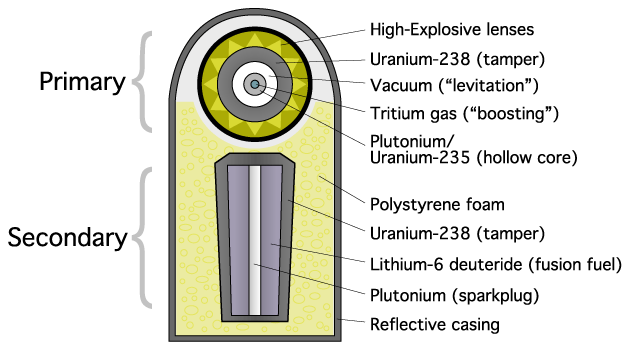
\includegraphics[scale=0.45]{./figures/Ulam_device.png}
  \caption{Schematic representation of the design of a thermonuclear weapon \cite{WikimediaCommons2005}.}
  \label{fig:ulam_device}
\end{figure}




The basic process of detonation is as follows: The primary device triggers first and supplies x-rays, which heat the secondary device, which heats the polystyrene foam into a plasma. The Plutonium \enquote{spark plug} at the center of the fusion assembly begins to undergo fission due to the compression from the polystyrene plasma. The Lithium-6 deuteride blanket, which surrounds the plutonium spark plug, produces tritium and begins the fusion stage. The flux of neutrons from the fusion reactions causes the \ce{^{238}U} tamper to undergo fission. At this stage the device breaks apart and a detonation is complete \cite{Defense1998}. 

Thermonuclear weapons are far more sophisticated than fission weapons, and essentially consists of three fission devices and one fusion device. It is assumed that ISIL is pursuing nuclear weapons in order to commit acts of terrorism. While higher yields will result in larger damage,  optimizing yield does not necessarily enhance the terror factor of a nuclear device. Due to the complexity of the design of multistage thermonuclear devices, it is assumed that ISIL will elect to pursue  fission weapons, most probably a gun-type design. 







\chapter[Appendix E: Technology]{Technology} \label{app:tech}


\section{Fission Weapons}
 
   \subsection{Passive Signals}

Passive signals for nuclear materials include the gamma rays that are given off during natural radioactive decay of the material, and neutrons that result either from spontaneous fission or (\(\alpha\),n) nuclear reactions (the \(\alpha\) particle comes from natural \(\alpha\) decay). The two most likely and common types of material that could be used for a nuclear weapon are highly enrich \ce{^{235}U} and highly enriched \ce{^{239}Pu}, and so these materials will be considered for passive detection. Weapons grade Uranium has a very low rate of released neutrons, and so detection by gamma rays would be recommended. Weapons grade Plutonium releases both, a large amount of neutrons and gamma rays and so both methods of detection are possible. 

The time needed to get acceptable detection by use of neutron and gamma counters varies based on distance and materials. \autoref{fig:det_time} shows an conservative estimate of the distance a mobile detector would need to be to get confirmation data that is 5 standard deviations above the background radioactivity. 


\begin{figure}
 \centering
 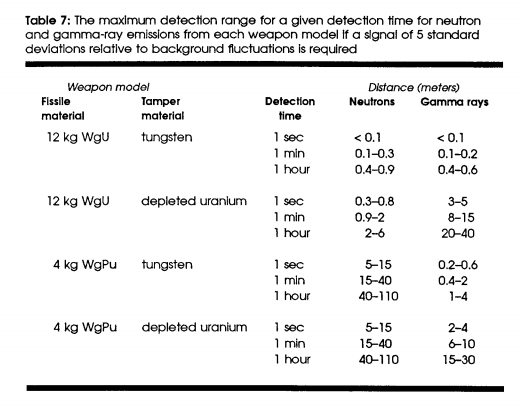
\includegraphics[trim = 0cm 0cm 0cm 2cm, clip,scale=0.6]{./figures/det_time.png}
   \caption{Table of distance and time needed to detect Weapons Grade  material with a tamper, where detection is considered when the counts are 5 standard deviations above the background. \cite{Fetter1990}}
     \label{fig:det_time}
\end{figure}


Passive gamma detection of weapons grade plutonium and uranium with a tungsten tamper are unlikely as the distance for detection is too small, even for a long detection count of 1 hour (\autoref{fig:det_time}). Passive neutron detection of weapons grade uranium is also unlikely for the same reasons. 


While the other weapon models have a fair distance of detection for a short time, the data does not take into account, additional shielding. To prevent detection by neutrons for a one minute detection period and one meter distance from the source, only 20 cm thick layer of lithium hydride would be needed \cite{Fetter1990}. To counter this, long detection period (\textgreater 10 minutes) \cite{Fetter1990} would be needed. Avoid detection of the gamma rays is significantly more difficult. The most likely and effective material to block gamma rays is lead. In order to bring the required detection period from 1 meter away to a time greater than 5 minutes, at least 100 kg of lead would be needed (see \autoref{fig:shield_time}).


\begin{figure}
 \centering
 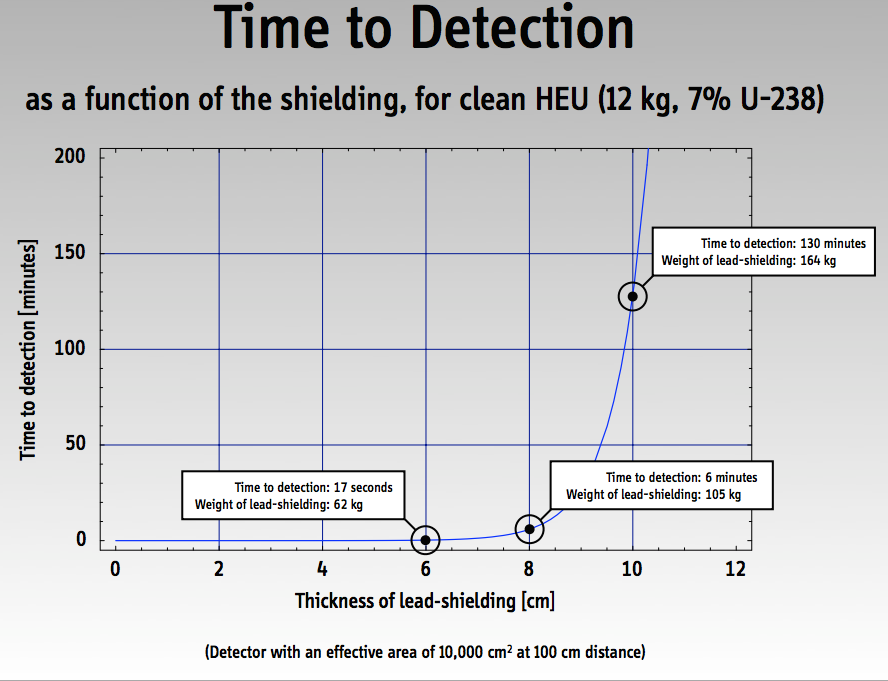
\includegraphics[trim = 0cm 0.1cm 0cm 0cm, clip,scale=0.4]{./figures/shield_time.png}
   \caption{Time needed to reach a gamma count of highly enriched uranium  5 standard deviations above the background for a given lead shield thickness \cite{Glaser2007}.}
     \label{fig:shield_time}
\end{figure}



If short detection time periods are needed, then it is unlikely that passive signals could be effectively utilized. If longer detection time are able to be done, then gamma detection of weapons grade plutonium and uranium with a depleted uranium tamper are possible with distances greater than or equal to 1 meter away. However, the requirement of the tamper material to be depleted uranium makes this method of detection highly not recommended, as or tamper materials such as tungsten are not significantly less likely to be used. 



\subsection{Active Signals}


% \myparagraph{Introduction to Active Interrogation}
\subsubsection{Introduction to Active Interrogation} \label{sec:intro_active_interrogation}


Active interrogation is a technique where an interrogating beam of neutrons or x-rays is used to scan a container in order to excite a response signal in special nuclear material. There are many different methods of active interrogation, which involve scanning the sample with different types of particles and measuring the resulting x-rays or gamma rays emitted by the material which was scanned.

Active interrogation can accurately identify special nuclear material. Furthermore, given the many methods of active interrogation, it is harder to shield against than passive detection.

While, active interrogation is a very good way to detect shielded nuclear material that is undetectable by passive interrogation, it does have two primary problems. The first, comes from the problem of illegal immigrants using cargo containers to enter a country through its ports. If the dose from active interrogation is high enough, the interrogation could result in the deaths of any potential stowaways \cite{Morse2014}. The second, is a logical conclusion that can be drawn from the definition of active interrogation. Namely, it involves shooting a beam at a target and waiting for a reaction. This obviously takes longer than simply measuring if any radiation comes off of a container. Thus, it is very likely not possible to use active interrogation on every container at a port, without slowing down commerce.

\subsubsection{Nuclear Resonance Fluorescence}

Nuclear Resonance Fluorescence is a method of active interrogation that involves hitting a target with high energy X-rays. This causes special nuclear material to enter an excited state, which will de-excite and give off a fluorescence gamma ray which can be detected. These fluorescence gamma rays are unique to each isotope allowing for positive identification \cite{Morse2014a}. The signatures expected from \ce{^{235}U} and \ce{^{239}Pu} are given in \autoref{tab:fluor_gammas}.

The main benefit of this method of active interrogation is that it works through several inches of steel or lead and several feet of hydrogenous material, which passive detection does not \cite{PhysRevC.78.041601}. Another interesting benefit is that this method of active interrogation can detect not only fissionable materials, but also any isotope larger than helium \cite{Bertozzi2005}.

This method of interrogation is able to function with very few counts. For example if the material gives of 20 counts, and the detector threshold is set at 17, meaning it alerts whoever is monitoring it when it receives 17 counts, this method has an efficiency of 99\% and a false positive rate of only 1\% \cite{Chichester2009}. 

\begin{figure}
 \centering
 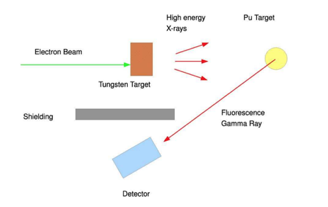
\includegraphics[trim = 0cm 0cm 0cm 0cm, clip,scale=0.7]{./figures/NRF_setup.png}
   \caption{A typical set-up for  a nuclear resonance fluorescence system \cite{Morse2014a}.}
     \label{fig:NRF_setup}
\end{figure}




% Please add the following required packages to your document preamble:
% \usepackage{multirow}
\begin{table}
\centering
\begin{tabular}{|c|c|c|}
\hline
Isotope                 & Transition    & Statistical Significance \\ \hline
\multirow{9}{*}{\ce{^{235}U}}   & 1656.23(80)   & 5.8                      \\ \cline{2-3} 
                        & 1687.26(33)\footnotemark[1]  & 10.2                     \\ \cline{2-3} 
                        & 1733.60(22)\footnotemark[1]  & 56.4                     \\ \cline{2-3} 
                        & 1769.16(28)\footnotemark[2] & 9.3                      \\ \cline{2-3} 
                        & 1815.31(22)\footnotemark[2] & 19.9                     \\ \cline{2-3} 
                        & 1827.54(23)   & 13.3                     \\ \cline{2-3} 
                        & 1862.31(20)   & 20.1                     \\ \cline{2-3} 
                        & 2003.32(25)   & 14.5                     \\ \cline{2-3} 
                        & 2006.19(31)   & 7.2                      \\ \hline
\multirow{12}{*}{\ce{^{239}Pu}} & 2040.25(21)   & 5.8                      \\ \cline{2-3} 
                        & 2046.89(31)   & 4.2                      \\ \cline{2-3} 
                        & 2135.00(37)\footnotemark[1]  & 3.5                      \\ \cline{2-3} 
                        & 2143.56(13)\footnotemark[1]  & 9.7                      \\ \cline{2-3} 
                        & 2150.98(31)\footnotemark[1]  & 4.2                      \\ \cline{2-3} 
                        & 2289.02(25)   & 6.2                      \\ \cline{2-3} 
                        & 2423.48(22)\footnotemark[2] & 7.2                      \\ \cline{2-3} 
                        & 2431.66(25)\footnotemark[2] & 6.3                      \\ \cline{2-3} 
                        & 2454.37(26)   & 6.2                      \\ \cline{2-3} 
                        & 2460.46(37)   & 4.7                      \\ \cline{2-3} 
                        & 2464.60(30)   & 5.7                      \\ \cline{2-3} 
                        & 2471.07(34)   & 4.6                      \\ \hline
\end{tabular}
\caption{Fluorescence Gamma Rays Given off by Isotopes of Concern \cite{PhysRevC.78.041601}.}
\label{tab:fluor_gammas}
\end{table}

\footnotetext[1]{Line pairs which are separated by 46.2 keV implying that one of the decays goes to a ground state while the other is to an excited state with an energy of 46.2 keV \cite{Bertozzi2005}. Furthermore, \ce{^{233}U} and \ce{^{237}Np} are not included here because of the low probability that they would be used in a device obtained by ISIL.}

\footnotetext[2]{Another set of line pairs separated by 46.2 keV implying that one of the decays goes to a ground state while the other is to an excited state with an energy of 46.2 keV \cite{Bertozzi2005}.}




\subsubsection{Neutron Interrogation}

Neutron interrogation involves hitting a target with a pulsed beam of neutrons in order to induce fission in target fissile material. Once fissions occurs, prompt and delayed neutrons and photons are emitted from the sample and may be detected. The characteristic energies of the neutrons and photons reveal the identity of the material \cite{Chichester2009}.  \autoref{fig:Chichester_timing}  shows the general pattern of responses to this type of interrogation while representative count rates for special nuclear material shielded by wood. Furthermore specific signatures to that can be expected from \ce{^{235}U} and \ce{^{239}Pu} can be found in \autoref{tab:neutron_signatures}.

The primary advantage of this technique is is that the systems are very small (\textless\ 0.2 m\(^3\)), light weight (\textless\ 12 kg), and use very little power (\textless\ 50 W) \cite{Chichester2009}.  Another major benefit is that research indicates this method will not subject the cargo to an excessive dose of radiation \cite{Hall2007}.  Research is still being conducted to determine if this method will work for a full size ago container \cite{Hall2007}.  A second major downside is that current technology requires the sample to be less than a meter from the detector, approximately 91.4 cm \cite{Hall2007}. Because this method works by inducing fissions, it is only able to detect fissionable material.



\begin{figure}
 \centering
 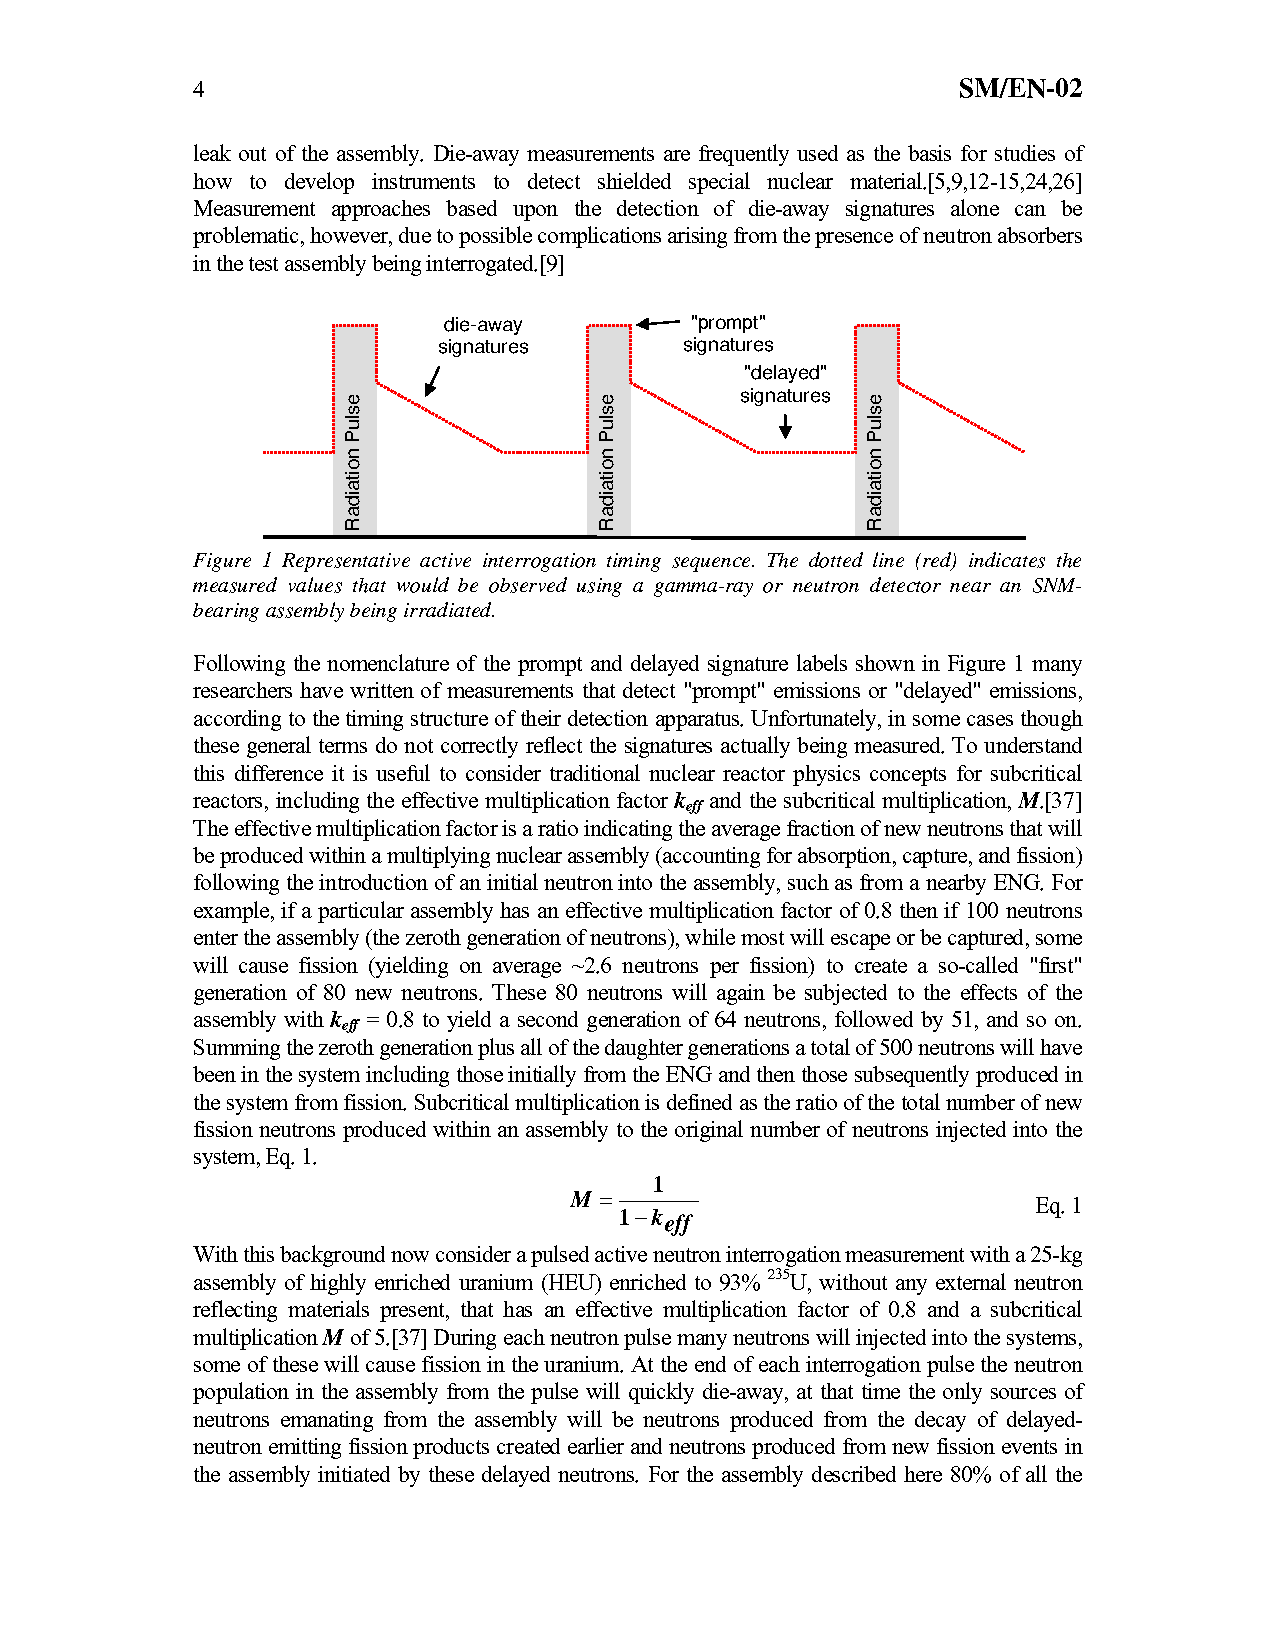
\includegraphics[trim = 5cm 18.7cm 5cm 5cm, clip,scale=1]{./figures/Chichester_timing.pdf}
   \caption{Representative pattern for pulsed neutron beam and when specific signatures can be expected \cite{Chichester2009}.}
     \label{fig:Chichester_timing}
\end{figure}


\begin{figure}
 \centering
 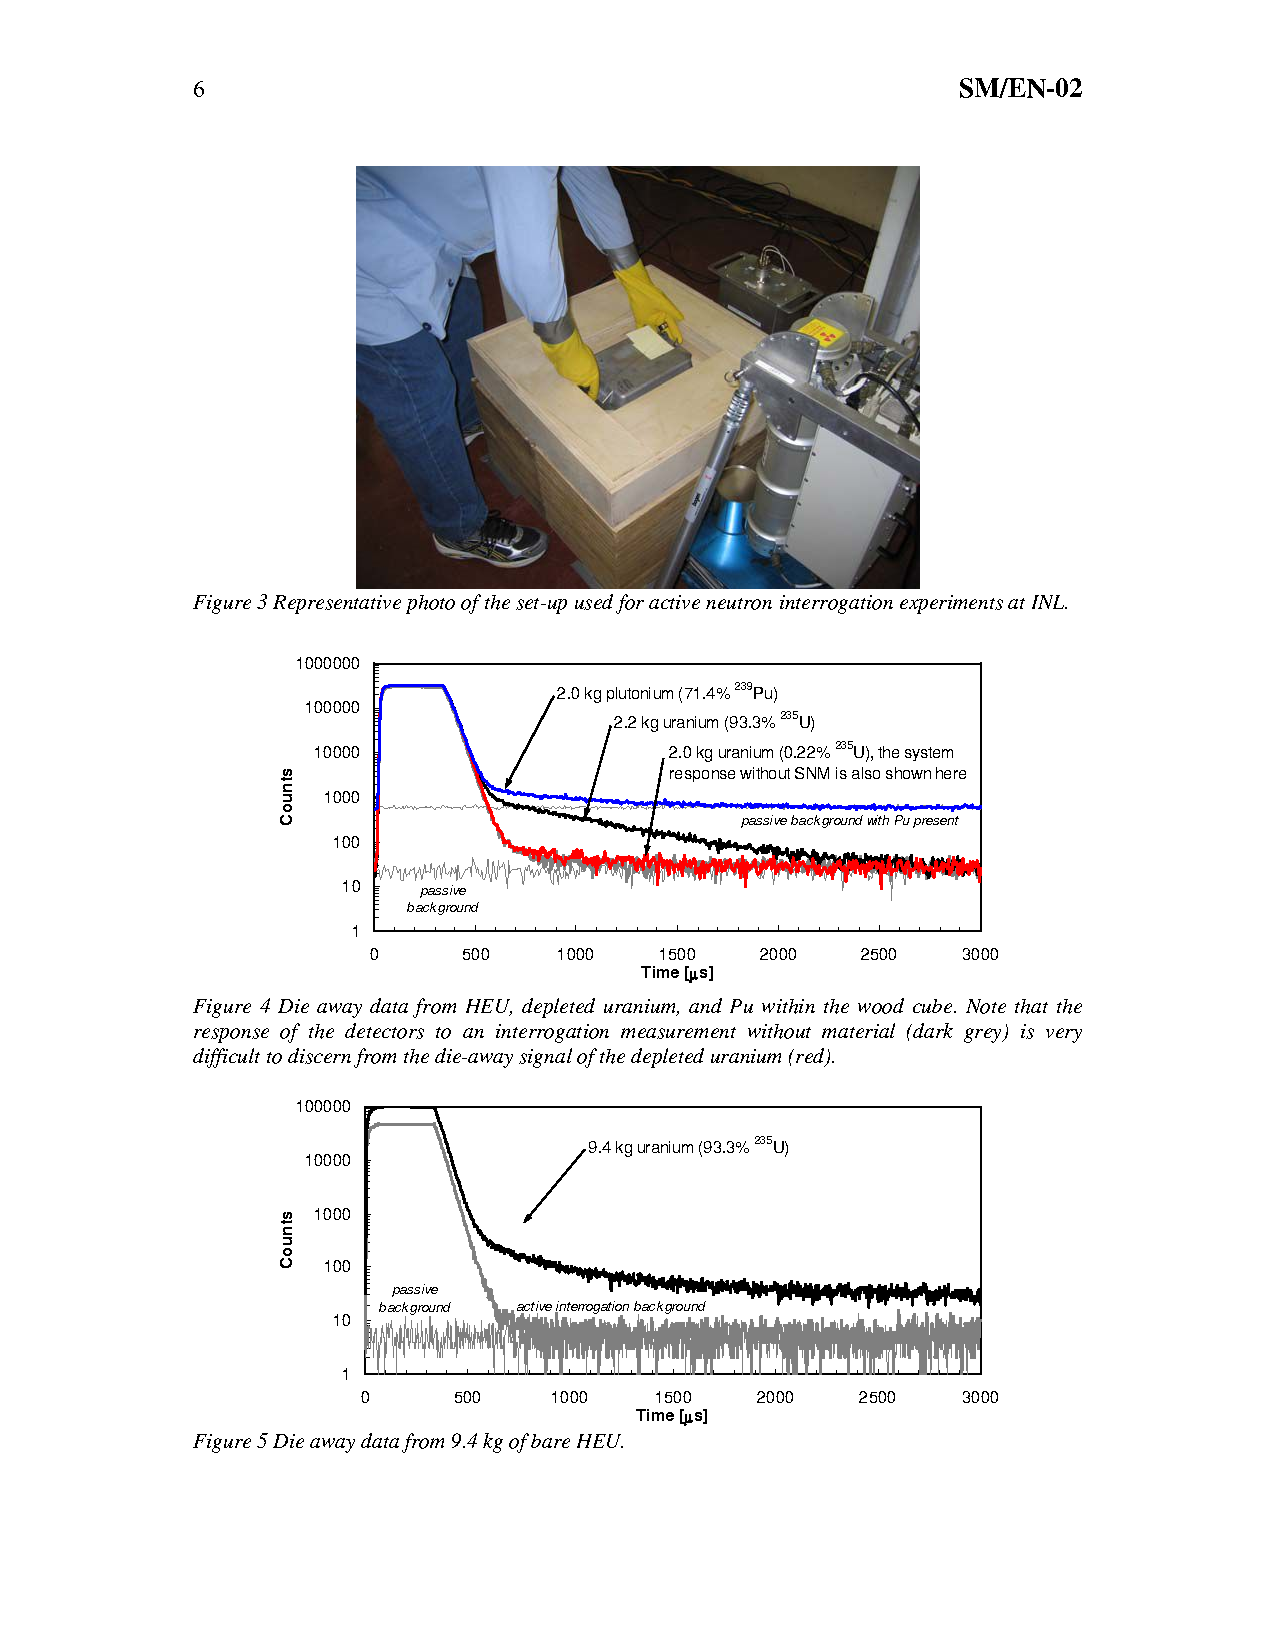
\includegraphics[trim = 3cm 11.3cm 3cm 10.5cm, clip,scale=1]{./figures/Chichester_counts.pdf}
   \caption{Counts over time for HEU, depleted uranium, and Pu in a wooden cube \cite{Chichester2009}.}
     \label{fig:Chichester_counts}
\end{figure}



As can be seen in \autoref{fig:Chichester_counts}, counting times necessary to identify samples are not incredibly long and can be under a minute \cite{Chichester2009}.




\begin{table}
\centering
\begin{tabular}{|c|c|c|}
\hline
Parameter                                                                                                                & \ce{^{235}U}                                                                                               & \ce{^{239}Pu}                                                                                               \\ \hline
\begin{tabular}[c]{@{}c@{}}Average Prompt Neutron Yield (multiplicity)\footnotemark[4]\\ (prompt neutrons per fission)\end{tabular}   & \begin{tabular}[c]{@{}c@{}}2.43 (thermal) \\ 2.57 (fission spectrum) \\  4.6 (14 MeV)\end{tabular} & \begin{tabular}[c]{@{}c@{}}2.87 (thermal) \\  3.09 (fission spectrum) \\  4.9 (14 MeV)\end{tabular} \\ \hline
\begin{tabular}[c]{@{}c@{}}Average Prompt Neutron Energy\footnotemark[5]\\ (MeV)\end{tabular}                                         & \begin{tabular}[c]{@{}c@{}}1.935 (thermal) \\  2.03 (14 MeV)\cite{PhysRevC.69.034607}\end{tabular}                       & \begin{tabular}[c]{@{}c@{}}2.010 (thermal) \\  2.19 (14 MeV)\cite{PhysRevC.69.034607}\end{tabular}                        \\ \hline
\begin{tabular}[c]{@{}c@{}}Average Prompt Photon Yield\\ (prompt photons per fission)\end{tabular}                       & 6.60\(\pm\)0.2 (thermal)\cite{Valentine2001}                                                                            & 7.06\(\pm\)0.2 (thermal)\cite{Valentine2001}                                                                             \\ \hline
\begin{tabular}[c]{@{}c@{}}Average Prompt Photon Energy\footnotemark[6]\\ (MeV)\end{tabular}                                          & 0.97\(\pm\)0.04 (thermal)\cite{Valentine2001}                                                                           & 0.95\(\pm\)0.04 (thermal)\cite{Valentine2001}                                                                            \\ \hline
\begin{tabular}[c]{@{}c@{}}Average Delayed Neutron Yield (multiplicity)\footnotemark[4]\\ (delayed neutrons per fission)\end{tabular} & \begin{tabular}[c]{@{}c@{}}0.0158 (thermal) \\  0.0165 (1.45 MeV)\end{tabular}                     & \begin{tabular}[c]{@{}c@{}}0.0061 (thermal) \\  0.0063 (1.45 MeV)\end{tabular}                      \\ \hline
Average Delayed Neutron Energy (MeV)                                           & 0.43                                                                                               & 0.4                                                                                                 \\ \hline
\begin{tabular}[c]{@{}c@{}}Average Delayed Photon Yield\footnotemark[7]\\ (delayed photons per fission)\end{tabular}                  & \begin{tabular}[c]{@{}c@{}}0.613 (short period) \\  3.31 (long period)\end{tabular}                & \begin{tabular}[c]{@{}c@{}}0.608 (short period) \\  3.26 (long period)\end{tabular}                 \\ \hline
Average Delayed Photon Energy (MeV)\footnotemark[8]                                         & 0.96                                                                                               & 0.98                                                                                                \\ \hline
\end{tabular}
\caption[Signatures from Active Neutron Interrogation \cite{Chichester2009}]{Signatures from Active Neutron Interrogation \cite{Chichester2009} \footnotemark[3]}
\label{tab:neutron_signatures}
\end{table}

\footnotetext[3]{Parentheses following certain values indicate fissions induced by neutrons of that specific energy}
\footnotetext[4]{Yields change based on the energy of the neutron that causes the fission}
\footnotetext[5]{Increases of approximately 4\% are expected for average neutron fission energies when going from thermal-neutron induced fission to fission-spectrum induced fissions}

\footnotetext[6]{Less than 2\% of these photons have energies larger than 2 MeV}
\footnotetext[7]{Delayed photon yields were measured over two counting periods. A short one, 0.2 s \textless t \textless 0.5 s and a long one, 0.2 s \textless t \textless 45 s.}
\footnotetext[8]{Energies averaged over the long counting period. Less than 1.8\% of the photons have energies greater than 2.3 MeV}



\section{Strategies for Detecting RDD}
 

The types of radioactive signals emitted from the \enquote{top 10} materials listed in \autoref{sec:RDD} are summarized here in \autoref{tab:RDD_signals}.  These passive radioactive signatures were acquired by various detection methods, with the most typical being the High Purity Germanium (HPGe) detectors and associated detector signal amplification and diagnostic tools \cite{Glaser2007}.  For each isotope, the radiation types are listed, some of primary energy levels for emitted particles based on laboratory testing results or other available references are included, and the total mass of a pure source which emits 1 petabecquerel (10\(^{15}\) Bq) of activity was calculated for inclusion. 




\begin{table}
\centering
\begin{tabular}{|l|c|l|l|}
\hline
\multicolumn{1}{|c|}{Isotope} & \multicolumn{1}{c|}{Type of emission} & \multicolumn{1}{c|}{\begin{tabular}[c]{@{}c@{}}Energy of emission \\ peak(s) {[}keV{]}\end{tabular}} & \multicolumn{1}{c|}{\begin{tabular}[c]{@{}c@{}}Material mass required \\ for producing  1 PBq \\ of Activity {[}g{]} (lbs)\end{tabular}} \\ \hline
\ce{^{241}Am}                         & \(\alpha\)                                 & 59.54                                                                                               & 7871.27 (17.353)                                                                                                                         \\ \hline
\ce{^{137}Cs}                         & \(\beta\), \(\gamma\)                            & \begin{tabular}[c]{@{}l@{}}661.67 \\ 383.85 \\ 356.02 \\ 302.9 \\ 276.4 \\ 80.9\end{tabular}        & 312.06 (0.688)                                                                                                                           \\ \hline
\ce{^{131}I}                          & \(\beta\)                                  & 606                                                                                                 & 0.22 (0.0005)                                                                                                                            \\ \hline
\ce{^{192}Ir}                         & \(\beta\), \(\gamma\)                            & 1459.7                                                                                              & 2.93 (0.006)                                                                                                                             \\ \hline
\ce{^{90}Sr}                          & \(\beta\)                                  & 546                                                                                                 & 195.56 (0.431)                                                                                                                           \\ \hline
\ce{^{3}H}                            & \(\beta\)                                  & 18.6                                                                                                & 2.81 (0.006)                                                                                                                             \\ \hline
\ce{^{60}Co}                          & \(\gamma\)                                 & \begin{tabular}[c]{@{}l@{}}1173.24 \\ 1332.5\end{tabular}                                           & 23.88 (0.053)                                                                                                                            \\ \hline
\end{tabular}
\caption{Summary of Radioactive Signal Emissions for RDD Isotopes of Concern}
\label{tab:RDD_signals}
\end{table}



The NRC defines LD50(30) to be the dose of radiation expected to cause death to 50 percent of an exposed population within 30 days (LD 50/30). Typically, the LD 50/30 is in the range from 400 to 450 rem (4 to 5 Sv) received over a very short period \cite{U}.  From this metric, the dose of 400 rem will be selected for evaluation here, and would require a very large source emission of radiation - typically one much larger than the practical release and yield of a RDD - and it will not occur over a very short period.

For passive detection of radiological materials, including isotope identification, gamma ray spectroscopy of radioactive emissions can be utilized with the development and deployment of aerial vehicle mounted radiological survey detectors \cite{Security2012}.







% \appendix
\chapter[Appendix F: Intelligence Overview]{Intelligence Overview}  \label{app:intel}


\section{Intelligence Collection \& Agency Responsibilities}

% \subsection{?????????  Generally speaking, this Appendix could use some references ???????????}

Intelligence agencies gather information from physical and technical observations, conversations, searches, and human operations. These sources are grouped into Signals Intelligence (SIGINT), Imagery Intelligence (IMINT), Measurement and Signature Intelligence (MASINT), Human-Source Intelligence (HUMINT), Open-Source Intelligence (OSINT) and Geospatial Intelligence (GEOINT) \cite{Intelligen}. The National Security Agency (NSA) is responsible for SIGINT, and the NSA collects SIGINT using signal communications between people, machines, and combinations of both. National Geospatial-Intelligence Agency (NGA) is responsible for the collection of IMINT using visual collection methods including cameras, radars, lasers, etc. MASINT is technically and scientifically based intelligence on unique attributes of the desired target. MASINT is the part of the Defense Intelligence Agency (DIA) and can be used to recognize, locate, and describe the target through nuclear, seismic, acoustic, material, radio frequency, and optical sciences. The Department of State, CIA, Department of Defense, Federal Bureau of Investigation, and other agencies use HUMINT sources, more commonly known as spies, to gather data via photography, document transfer, information download, etc. in enemy territory. OSINT relies on publicly available information, and a large synthesis of OSINT is performed at Foreign Broadcast Information Service (FBIS) and the National Air and Space Intelligence Center (NASIC). GEOINT belongs to the NGA and is generally collected from satellites and reconnaissance aircraft. 

\subsection{Information Classification}

The Information Security Oversight Office (ISOO) determines standards for information classification based on policy guidance from the National Security Council (NSC). ISOO has oversight of the extensive security characterization framework and the National Industrial Security Program. ISOO sets requirements for the original classification of information if the following apply: information should be classified by the classification authority; information is belongs to, controlled by, or is for the United States; information refers to one of the classification categories; classification authorities determines damage will be caused to national security from unsanctioned disclosure \cite{Office2010}. The classes of information classification believed to be effective \cite{Richelson2011,Office2010}.  The general classes of classification are:


\begin{itemize}
  \item Top secret: \enquote{exceptionally grave damage} to national security in case of disclosure.
  \item Secret: \enquote{serious damage} to national security in case of disclosure.
  \item Confidential: \enquote{damage} to national security in case of disclosure.
  \item Unclassified.
\end{itemize}

The information volume received from the all intelligence sources is astronomic. To facilitate the handling of this volume of information, assets are assigned based on the prioritization of the information. These are assigned as low, medium, and highly important:

\begin{itemize}
  \item \underline{Low (moderately serious)}: (e.g. planning to build weapon: enough time to plan actions and monitor progress).
  \item \underline{Medium (very serious)}: (e.g. weapon building in the process: actions should be taken ASAP).
  \item \underline{High (catastrophic)}: (e.g. weapon exists, ready to use: time is determining factor and actions should be taken immediately).
\end{itemize}

Combining these classification categories, a set of information and its sensitivity for the ISIL nuclear threat can be generated and is shown in \autoref{tab:separate_sec_level}.  

% \subsubsection{?????? Be good to color code according to TS, S, C, or unclassified ???????}

% Please add the following required packages to your document preamble:
% \usepackage[table,xcdraw]{xcolor}
% If you use beamer only pass "xcolor=table" option, i.e. \documentclass[xcolor=table]{beamer}
\begin{table}
\centering
\begin{tabular}{|c|l|c|c|c|}
\hline
\multicolumn{2}{|c|}{Information Category}           & \multicolumn{3}{c|}{Minimum Security Level}                                                 \\ \hline
\# & \multicolumn{1}{c|}{Information type}           & \cellcolor[HTML]{34FF34}LOW & \cellcolor[HTML]{FCFF2F}MEDIUM & \cellcolor[HTML]{FE0000}HIGH \\ \hline
1  & Information about weapon                        & \cellcolor[HTML]{34FF34}    & \cellcolor[HTML]{FCFF2F}X      & \cellcolor[HTML]{FE0000}     \\ \hline
2  & Information about weapon location               & \cellcolor[HTML]{34FF34}    & \cellcolor[HTML]{FCFF2F}       & \cellcolor[HTML]{FE0000}X    \\ \hline
3  & Information about target                        & \cellcolor[HTML]{34FF34}    & \cellcolor[HTML]{FCFF2F}       & \cellcolor[HTML]{FE0000}X    \\ \hline
4  & Information about persons related to the weapon & \cellcolor[HTML]{34FF34}    & \cellcolor[HTML]{FCFF2F}X      & \cellcolor[HTML]{FE0000}     \\ \hline
\end{tabular}
\caption{Separation of information by minimum security levels.}
\label{tab:separate_sec_level}
\end{table}

\subsection{International Intelligence Sharing}

Information sharing in the international IC is immensely more complicated than between internal U.S. agencies. The mere fact of declared opposition to ISIL is an insufficient basis for intelligence sharing alone.  Indeed, the U.S. has  various strained relationships with many allies in the fight against ISIL. It is assumed that information sharing on the ISIL issue would fall along lines consistent with historical cooperation levels. Cooperation levels can be divided into a simple system of three levels as shown in \autoref{tab:relation_table}.




\begin{table}[h]
\centering
\begin{tabular}{|c|l|}
\hline
Levels & \multicolumn{1}{c|}{Definition}                                                                                                             \\ \hline
1      & Historically and currently close relationship (Great Britain, France, Canada)                                                    \\ \hline
2      & \begin{tabular}[c]{@{}l@{}}Neither good nor bad relations or recent downturn in relations \\ For example: Germany as neutral \cite{BBC2013} and Israel as recent downturn \cite{Goldberg2014}.\end{tabular} \\ \hline
3      & Historically and currently bad relationship (Russia, Jordan, Turkey, Egypt \cite{Office2010})                                                  \\ \hline
\end{tabular}
\caption{Intelligence sharing cooperation levels for the U.S. }
\label{tab:relation_table}
\end{table}



After Edward Snowden promulgated the snooping actions of the U.S. Intelligence community into its allies, Germany decided to close \enquote{friendly} intelligence cooperation \cite{BBC2013}. Consequently, it would be hard to reach an open relationship in intelligence cooperation so soon after the Snowden case. Countries in the Level 3 category were chosen because of their lack of close political relationships with the U.S., unlike the countries in Level 1 and 2. 


A good example of informal multilateral agreement amongst level one countries is the United Kingdom - United States of America Agreement for cooperation in intelligence gaining between five English-speaking democracies: the United Kingdom, the United States, Canada, Australia and New Zealand \cite{Cox2012}. The collaboration began during World War II to track German and Russian signals and activities and endured for 70 years. The agreement enables the members to share intelligence facilities, avoid duplication, and combine strength. The U.S. and the UK have the most advanced technical abilities, biggest budgets, and are main players in the alliance. The U.S. operates intelligence centers in allied countries: one of the world's largest eavesdropping centers in Britain is run by NSA with hundreds of British employees from the Government Communications Headquarters (GCHQ); Pine Gap, a satellite tracking station in Australia, is run Partly run by the CIA, NSA, and U.S. National Reconnaissance Office (NRO). The agencies work side-by-side, allowing information flow quickly. The members of the alliance work with foreign intelligence to obtain local information without letting them into the alliance. Only U.S. intelligence officers can directly access the database; other country members have to show potential links to U.S. security threats for the information they request from the database. All members have benefited from the information sharing. The U.S. and UK prevented a major attack in 2006 designed to use liquid explosives to explode 10 airliners traveling from the UK to U.S. and Canadian destinations. 


\chapter[Appendix G: International Partnerships]{International Partnerships} \label{app:partners}

\section{Strategic Communication }

% \subsection{????????  This appendix needs references  ???????}


Strategic communication became increasingly important with the advent of globalization and interconnectivity (borderless world) that led to rising threats from \enquote{transnational} issues. Security challenges no longer come in lone tangible entities, but instead are multi-polar and dispersed into gray areas where there are no clear cut answers, everything is connected, and second order effects must be accounted for. Strategic communication was developed to provide a framework to help solve the multi-polar problem that defines our current security environment.

Communications or exchanges of information (intelligence sharing) can be on the bilateral or multilateral level. Cooperating at the multilateral level diversifies sources of intelligence and increases the confidence in intelligence assessments. Multilateralism disproportionally benefits smaller countries with less bargaining power and resources, but working together with these countries can be effective in tackling issues of concern related to nuclear proliferation that may utilize black markets and networks that reside in their country. On the other hand, multilateral cooperation requires a complex system requiring organization and structure to ensure timely and accurate sharing of information. Additionally, the large number of participants can result in lower security of information thereby affecting the willingness of countries to share confidential and sensitive materials.

At the bilateral level, both sides can be more specific and develop tailored agreements. From a liberalism perspective, bilateralism can help larger states gain control over smaller states through a series of arrangements that maximize the influence of the larger state. However, bilateral cooperation can be more wasteful in time and effort as compared to a multilateral strategy. It can also be less reliable because no international norm is established creating compliance pressure, which can lead to compliance with the agreement becoming a bargaining chip to gain further concessions.

The U.S. sees merits in pursuing both multilateral and bilateral effort in international strategic communications. Most of the times, the U.S. tends to favored intense bilateralism over multilateralism to achieve its objectives. However, following World War II, multilateral initiatives in the area of nuclear non-proliferation and disarmament increased in significance.  This multilateral transition was marked by the creation of the United Nations (UN) in 1945.  The UN, and several subsequent agencies, are the current approach taken by the U.S. to address nuclear proliferation concerns.  

\subsection{Nuclear-Relevant Organizations }

The UN is the largest international organization that can take actions on the issues of security at a global level. Several divisions in the UN address nuclear security issues including the General Assembly (GA), the Security Council (SC), and the Department of Disarmament Affairs (DDA). The GA can make recommendations to Member States and the SC about situations that are likely to endanger international peace and security. The SC consists of five permanent member states (China, France, Russia, United Kingdom, and the United States) and 10 non-permanent members. The Security Council is responsible for formulating plans for the regulation of armaments. The DDA provides substantive and organizational support to UN Member States for disarmament norm-setting through the work of the GA and other bodies. The DDA's WMD Branch supports multilateral efforts to strengthen the international norm on disarmament and non-proliferation of WMD and cooperates with other UN agencies, such as the IAEA.

The IAEA was established in 1957, with the aim of promoting peaceful uses of nuclear energy through safeguards \cite{InternationalAtomicEnergyAgency}. The IAEA maintains the legal framework and technical capabilities to establish and verify the safeguards agreements with Non-Proliferation Treaty (NPT) member states. IAEA is authorized to conduct inspections of a NPT member country's declared and undeclared nuclear facilities. If a state is caught in non-compliance with its safeguards agreements, the Board of Governors has the right to ask for more information and may refer it to the UN Security Council for further action. However, the power of IAEA is limited to the countries that have signed NPT, and the scope of inspection is limited as defined in the safeguard agreement. 








\chapter[Appendix H: Bilateral Relations between the U.S. \& Strategic Countries]{Bilateral Relations between the U.S. \&  Strategic Countries} \label{app:relations_table}

As a concise summary of U.S. foreign relations (as they relate to ISIL acquisition of nuclear weapons), a matrix of Bilateral Relations between the U.S. and Strategic Countries is provided in \autoref{tab:bilateral_table}.


% \afterpage{
\begin{landscape}
% Please add the following required packages to your document preamble:
% \usepackage{graphicx}
\begin{table}
\centering
\resizebox{1.38\textwidth}{!}{%
\begin{tabular}{|l|l|l|l|}
\hline
\multicolumn{1}{|c|}{Country}                               & \multicolumn{1}{c|}{Relationship with U.S.}                                                                                                                                                                                                                                                                                                                                                                                               & \multicolumn{1}{c|}{Military and Nuclear Capabilities}                                                                                                                                                                                                                                                                                                        & \multicolumn{1}{c|}{ISIL Position}                                                                                                                                                                                                                                                                                                                                                                      \\ \hline
Russia                                                      & \begin{tabular}[c]{@{}l@{}}Strained relationship due to economic sanctions, imposed for Russia's annexation of Crimea.\\ Predicted power struggle for new world order, and a historical rival.\\ Agreed to maintain dialogue in areas of terrorism, energy security, and\\ 			nuclear non-proliferation issues (Iran, North Korea).\end{tabular}                                                                                        & \begin{tabular}[c]{@{}l@{}}Military capability rank: 2 \cite{U.S.CentralIntelligenceAgency2012} (after the U.S.)\\ Defense spending: U.S.\$84.5 billion (2014) \cite{StockholmInternationalPeaceResearchInstitute2014}\\ Total NW inventory: 7,500; deployed strategic: 1,780 \cite{FederationofAmericanScientists2015}\end{tabular}                                                                                                                                               & \begin{tabular}[c]{@{}l@{}}More than 500 Russians are believed to have joined ISIL.\\ Russia considering supplying military equipment to Libya and Iraq. Agreed\\ 			to work together with  U.S. on facing ISIL.\end{tabular}                                                                                                                                                                             \\ \hline
China                                                       & \begin{tabular}[c]{@{}l@{}}China and the U.S. have a close economic partnership. \\ Two-way trade between China and the United States is \\ over U.S.\$590 billion in 2014. China is the second largest export country (after Canada).\end{tabular}                                                                                                                                                                                         & \begin{tabular}[c]{@{}l@{}}Military capability rank: 3 \cite{U.S.CentralIntelligenceAgency2012}\\ Defense Spending: U.S.\$145 billion (2014)\\ China has been increasing its annual military budget \\ over the last two decades. Total NW inventory: 250; deployed strategic: 0 \cite{StockholmInternationalPeaceResearchInstitute2014}\end{tabular}                                                                                            & \begin{tabular}[c]{@{}l@{}}Chinese Muslim Uyghur militants trying to flee the country and join ISIL\\ 			training camps in preparation for attacks back home.\end{tabular}                                                                                                                                                                                                                              \\ \hline
\begin{tabular}[c]{@{}l@{}}United\\ 			Kingdom\end{tabular} & \begin{tabular}[c]{@{}l@{}}Special relationship; close allies encompassing various issues, \\ including political and military, dating back to Churchillian era.\end{tabular}                                                                                                                                                                                                                                                           & \begin{tabular}[c]{@{}l@{}}Military capability rank: 5 \cite{U.S.CentralIntelligenceAgency2012} \\ Defense Spending: U.S.\$51.5 billion (2014) Talks of spending reduction.\\ Total NW inventory: 225; deployed strategic: 160 \cite{FederationofAmericanScientists2015}\end{tabular}                                                                                                                                              & \begin{tabular}[c]{@{}l@{}}The U.K. government declared ISIL a terrorist organization.\\ Hundreds of U.K. citizens are estimated to have joined ISIL.\\ 			U.K. citizens have been killed or kidnapped by ISIL.\end{tabular}                                                                                                                                                                            \\ \hline
France                                                      & \begin{tabular}[c]{@{}l@{}}France is the U.S.' oldest ally, relationship remains active and friendly. \\ 			France supported U.S. on various issues, but France was skeptical of U.S. invasion of Iraq.\end{tabular}                                                                                                                                                                                                                    & \begin{tabular}[c]{@{}l@{}}Military capability rank: 6 \cite{U.S.CentralIntelligenceAgency2012} \\ 			Defense spending: U.S.\$40 billion (2014)\\ 			Total NW inventory: 300; deployed strategic: 290 \cite{StockholmInternationalPeaceResearchInstitute2014}\end{tabular}                                                                                                                                                                       & \begin{tabular}[c]{@{}l@{}}France supported U.S.-led coalition against ISIL.\\ 			France's colonial history in Africa made it pivotal in the fight against\\ 			ISIL and Islamic terrorism in Africa. ISIL called for French\\ 			Muslim to join the group and perform terror attacks within France.\end{tabular}                                                                                         \\ \hline
\begin{tabular}[c]{@{}l@{}}North\\ 			Korea\end{tabular}    & \begin{tabular}[c]{@{}l@{}}North Korea has repeatedly threatened the U.S. with nuclear attacks.	\\  Relationship between the two countries are negative.		North Korea is not a party to NPT.\end{tabular}                                                                                                                                                                                                                               & \begin{tabular}[c]{@{}l@{}}Military capability rank: 36 \cite{U.S.CentralIntelligenceAgency2012} \\ 			Defense Spending: U.S.\$5.5 billion (2014) \cite{U.S.CentralIntelligenceAgency2012} \\ Total NW inventory: 6-8; deployed strategic: 0 \cite{StockholmInternationalPeaceResearchInstitute2014} \\ 			Recent reports suggest that North Korea may have up \\ to 20 nuclear warheads and could built as many as 100 by 2020 \cite{TheEditorialBoard2015a}.\end{tabular}                              & \begin{tabular}[c]{@{}l@{}}North Korea has publicly condemned U.S. effort in annihilating ISIL.\\ 			However, no concrete information has been gathered whether North\\ 			Korea and ISIL have made significant contact. U.S. worries North\\ 			Korea will sell nuclear technology to non-state actors.\end{tabular}                                                                                     \\ \hline
Israel                                                      & U.S. was the first country that that recognized independence of Israel in 1948.                                                                                                                                                                                                                                                                                                                                                         & \begin{tabular}[c]{@{}l@{}}Military capability rank: 11 \cite{U.S.CentralIntelligenceAgency2012}\\ 			Defense spending: U.S.\$17 billion (2014)\\ 			Total NW inventory: 80; deployed strategic: 0 \cite{StockholmInternationalPeaceResearchInstitute2014}.\end{tabular}                                                                                                                                                                          & \begin{tabular}[c]{@{}l@{}}Report from the UN reveals that the Israeli Defense Forces\\ (IDF) maintained regular contact with members of ISIL since May 2013.\end{tabular}                                                                                                                                                                                                                              \\ \hline
India                                                       & \begin{tabular}[c]{@{}l@{}} \enquote{Global strategic partnership} based on shared democratic values and\\ 			increasing convergence of interests on bilateral, regional and global issues. \\ Historically, India was close ally with Russia then\\ 			pioneered the Non-Aligned Movement (NAM).\end{tabular}                                                                                                                                   & \begin{tabular}[c]{@{}l@{}}Military capability rank: 4 \cite{U.S.CentralIntelligenceAgency2012}\\ 			Defense spending: U.S.\$38 billion (2014)\\ 			Total inventory: 90 - 100; deployed strategic: 0 \cite{StockholmInternationalPeaceResearchInstitute2014}.\end{tabular}                                                                                                                                                                       & \begin{tabular}[c]{@{}l@{}}ISIL identified Central Asia, including area north of India, as \enquote{a ripe recruitment area.} \\ 			The government considered ISIL as a periphery issue, but\\ 			ISIL's plan of expansion might include areas in India.\end{tabular}                                                                                                                                           \\ \hline
Pakistan                                                    & \begin{tabular}[c]{@{}l@{}}Over the decades, Pakistan has been a great ally to the U.S., but there\\ 			are instances where the two countries disagreed. U.S. views Pakistan \\ as its ally, but worries about the threat of terrorism in\\ 			Pakistan. Pakistan has received U.S.\$28.4 billion in military and non-military aid post 9/11.\end{tabular}                                                                                & \begin{tabular}[c]{@{}l@{}}Military capability rank: 17 \cite{U.S.CentralIntelligenceAgency2012}\\ 			Defense spending: U.S.\$7 billion (2014)\\ 			Pakistan is not a party to NPT.\\ 			Total NW inventory: Unknown.\end{tabular}                                                                                                                                                                & \begin{tabular}[c]{@{}l@{}}Many members of Pakistan's terrorist groups have joined ISIL. ISIL's leaked \\ secret memo spelled out the master plan on how to wage war\\ 			against the Pakistani military while trying to join forces with\\ 			local militants.\end{tabular}                                                                                                                            \\ \hline
Iran                                                        & \begin{tabular}[c]{@{}l@{}}Long and unpleasant history; current concerns about Iran are its\\ 			support for terrorism, pursuit of nuclear weapons, its opposition \\ towards Israelis and Arabs, and the country's poor human rights record.\end{tabular}                                                                                                                                                                             & \begin{tabular}[c]{@{}l@{}}Military capability rank: 23 \cite{U.S.CentralIntelligenceAgency2012}\\ 			Defense spending: U.S.\$6.3 billion (2014)\\ 			Currently, Iran and P5+1 countries are negotiating a nuclear deal to halt\\ 			Iran's nuclear development.\end{tabular}                                                                                                                    & \begin{tabular}[c]{@{}l@{}}Iran and ISIL are fighting for the crown of militant Islam. In this\\ 			case, our enemy's enemy is not our friend. The goal for the U.S. is to\\ 			defeat ISIL and to halt Iran's nuclear program.\end{tabular}                                                                                                                                                                  \\ \hline
Iraq                                                        & \begin{tabular}[c]{@{}l@{}}The Strategic Framework Agreement for a Relationship of Friendship and\\ 			Cooperation between the U.S. and the Republic of Iraq guides the\\ 			overall political, economic, cultural, and security ties with\\ 			Iraq.  This agreement is designed to help the Iraqi people stand\\ 			on their own and reinforce Iraqi sovereignty, while protecting 			U.S. interests in the Middle East.\end{tabular} & \begin{tabular}[c]{@{}l@{}}Military capability rank: 112 \cite{U.S.CentralIntelligenceAgency2012}\\ 			Defense spending: U.S.\$6 billion (2014)\\ 			The U.S. has been heavily investing in reforming and assisting the\\ 			country's military capabilities.\end{tabular}                                                                                                                          & \begin{tabular}[c]{@{}l@{}}ISIL is carving its territory from Iraq. The weak governance of Iraq\\ 			instigated ISIL's ambition. has been battling ISIL aided by a\\ 			coalition made up of Shiite militiamen and volunteers.\end{tabular}                                                                                                                                                             \\ \hline
Syria                                                       & \begin{tabular}[c]{@{}l@{}}The U.S.-Syria relationship is negative after having suspended diplomatic relations in 2014. \\ 			The U.S. has imposed economic sanction to Syria since 2004 due to\\ 			Syria's involvement in harboring terrorist groups. The U.S. is\\ 			deeply opposed to President Bashar al-Assad's regime,\\ 			specifically regarding chemical weapons use.\end{tabular}                                     & \begin{tabular}[c]{@{}l@{}}Military capability rank: 42 \cite{U.S.CentralIntelligenceAgency2012}\\ 			Defense spending: U.S.\$1.9 billion (2014)\\ Syrian's military hardware are mostly acquired from Russia and Iran.\\ 			Despite losing its military personnel, the Syrian military has been said\\ 			to become more flexible and capable especially in anti-guerrilla warfare.\end{tabular} & \begin{tabular}[c]{@{}l@{}}ISIL is gaining foothold in Syria, and carving its territory from the\\ 			country. Hence, Syrian government is fighting ISIL. The U.S. has\\ 			floated the idea to train the Syrian military opposition, and even\\ 			the Syrian military itself, in order to fight ISIL. Syria views\\ 			U.S.-led coalition against ISIL as a threat to their sovereignty.\end{tabular} \\ \hline
\end{tabular}
}
\caption{Matrix of Bilateral Relations between the U.S. and Strategic Countries}
\label{tab:bilateral_table}
\end{table}
\end{landscape}
% }
% \nopagebreak[4]


\newpage
\pagestyle{fancyTOC}


\addcontentsline{toc}{chapter}{Bibliography}
\bibliographystyle{ieeetr}
\bibliography{../../../library}
\thispagestyle{fancyTOC}


\end{document}
